% \sout sudah didefinisikan oleh paket ulem di preambel
%
% ATRIBUSI: Sebagian besar bab ini (motivasi tentang pemeriksa halaman dan K\"onigsberg,
% definisi, contoh algoritme Dijkstra dan pohon merentang, serta banyak
% latihan) diadaptasi dari bab "Graph Theory" dalam "Math in Society"
% karya David Lippman, berlisensi CC BY-SA 3.0 (http://www.opentextbookstore.com/mathinsociety/).
% Modifikasi oleh Robert Hildebrand dan para kontributor; dilisensikan ulang dengan CC BY-SA 4.0
% sebagai bagian dari buku ini. Lihat frontmatter/sources-attribution.tex.
\chapter{Algoritme Graf}\footnote{Sebagian besar isi bab ini, termasuk contoh-contoh pengantar, sejumlah penelusuran langkah demi langkah algoritme, dan beberapa latihan, diadaptasi dari bab Teori Graf dalam \emph{Math in Society} karya David Lippman, yang berlisensi CC BY-SA 3.0, dengan modifikasi oleh Robert Hildebrand dan para kontributor. Lihat bab Sumber dan Atribusi untuk perinciannya.}

\section{Teori Graf}
Di dunia modern, perencanaan rute yang efisien sangat penting bagi bisnis dan industri, dengan penerapan yang beragam seperti distribusi produk, pemasangan jalur serat optik baru untuk internet pita lebar, dan pemberian saran teman baru di situs jejaring sosial seperti Facebook.

Bidang matematika ini bermula hampir 300 tahun yang lalu dari penyelidikan sebuah teka-teki matematika (yang akan segera kita bahas).  Arti penting bidang ini meningkat pesat pada abad terakhir, baik karena bertambahnya kompleksitas bisnis dalam ekonomi global maupun karena daya komputasi yang disediakan komputer.  
\section{Graf}
\subsection{Menggambar Graf}

\begin{example}{}
Berikut adalah sebagian kawasan perumahan di Missoula, Montana\footnote{Sam Beebe. http://www.flickr.com/photos/sbeebe/2850476641/}.  Sebagai bagian dari pekerjaannya, pemeriksa halaman kawasan tersebut harus menyusuri setiap jalan di kawasan itu untuk memastikan bahwa penataan halaman para pemilik rumah memenuhi ketentuan komunitas.\\
\begin{center}
\scalebox{0.8}{
\altincludegraphics{graph-theory-graphics/GraphPicture.png}{Foto udara sebuah kawasan perumahan di Missoula, Montana, yang memperlihatkan beberapa blok rumah yang dihubungkan oleh jaringan jalan. Gambar ini memunculkan pertanyaan apakah seorang pemeriksa halaman dapat menyusuri setiap jalan tanpa harus kembali menelusuri jalan yang sama.}
}\par\captionof{figure}{Foto udara sebuah kawasan perumahan di Missoula, Montana, yang memperlihatkan beberapa blok rumah...}\label{fig:GraphPicture}% fig-num-auto

\end{center}

Tentu saja, ia ingin meminimalkan jarak yang harus ditempuhnya.  Mungkinkah ia menyusuri setiap jalan di kawasan ini tanpa harus kembali menelusuri jalan yang sama?  Walaupun Anda mungkin dapat menjawab pertanyaan itu hanya dengan mengamati gambar tersebut beberapa saat, akan lebih baik jika kita dapat menjawabnya untuk gambar apa pun, berapa pun tingkat kerumitannya.\\

Untuk melakukannya, pertama-tama kita perlu menyederhanakan gambar itu menjadi bentuk yang lebih mudah diolah.  Kita dapat menggambar sebuah garis sederhana untuk setiap jalan.  Di setiap perpotongan jalan, kita tempatkan sebuah titik. \\
 
 \altincludegraphics{graph-theory-graphics/GraphPictureDot.png}{Berdampingan: pada foto udara kawasan perumahan ditambahkan titik merah di persimpangan dan garis merah di sepanjang jalan; di sebelahnya, jaringan yang sama digambar ulang sebagai graf berupa simpul berlabel yang dihubungkan oleh sisi, sehingga memperlihatkan penyederhanaan peta jalan menjadi graf.}\par\captionof{figure}{Berdampingan: pada foto udara kawasan perumahan ditambahkan titik merah di persimpangan dan garis merah di sepanjang jalan...}\label{fig:GraphPictureDot}% fig-num-auto

\end{example}

Jenis gambar sederhana ini disebut \textbf{graf}.  

\begin{definition}{Graf, Simpul, dan Sisi}
Sebuah graf terdiri atas sekumpulan titik, yang disebut simpul, dan sekumpulan sisi yang menghubungkan pasangan-pasangan simpul.  
\end{definition}

Walaupun graf semula kita gambar agar sesuai dengan gambar yang tersedia, tata letaknya tidak memiliki arti khusus ketika kita menganalisis graf.  Kedua graf di bawah ini ekuivalen dengan graf yang digambar di atas karena keduanya memperlihatkan hubungan sisi yang sama di antara simpul-simpul yang sama seperti pada graf semula.

 
\begin{minipage}{0.49\textwidth}
\begin{tikzpicture}
    \foreach \pos/\name in {{(0,0)/A}, {(1,0)/D}, {(2,0)/G}, {(3,0)/N}, {(4,0)/O}, {(1,1)/B}, {(2,1)/E}, {(3,1)/F}, {(4,1)/M}, {(3,2)/C}, {(2,-1)/H}, {(3,-1)/J}, {(2,-2)/I}, {(3,-2)/K}, {(4,-2)/P}, {(5,-2)/Q}, {(3,-3)/L}, {(5,-3)/R}}
                \node[vertex] (\name) at \pos {$\name$};
                
 \foreach \source/ \dest in {A/D, D/G, A/B, B/E, B/C, C/F, E/F, F/M, D/E, E/G, G/H, H/I, H/J, I/K, J/K, K/L, N/J, F/N, F/M, N/O, O/P, P/Q, Q/R, M/O, K/P, L/R}
              \path (\source) edge (\dest);                
\end{tikzpicture}\par\captionof{figure}{Graf kawasan perumahan dengan delapan belas simpul A sampai R yang ditata kurang lebih menyerupai kisi...}\label{fig:graphtheory-dor1-tikz01}% fig-num-auto
     
\end{minipage}
%
\begin{minipage}{0.49\textwidth}
\begin{tikzpicture}
    \foreach \pos/\name in {{(0,0)/A}, {(0,-1)/D}, {(0.6,-2.25)/G}, {(6,-1)/N}, {(3.5,2.5)/O}, {(.25,1)/B}, {(5.4,1.25)/E}, {(2.4,-3.5)/F}, {(4.6,2.25)/M}, {(1,1.75)/C}, {(1.4,-3.25)/H}, {(5.75,-2)/J}, {(6,0)/I}, {(3.5,-3.5)/K}, {(2.5,2.5)/P}, {(1.6,2.25)/Q}, {(4.4,-3.25)/L}, {(5,-2.75)/R}}
                \node[vertex] (\name) at \pos {$\name$};
                
 \foreach \source/ \dest in {A/D, D/G, A/B, B/E, B/C, C/F, E/F, F/M, D/E, E/G, G/H, H/I, H/J, I/K, J/K, K/L, N/J, F/N, F/M, N/O, O/P, P/Q, Q/R, M/O, K/P, L/R}
              \path (\source) edge (\dest);                
\end{tikzpicture}\par\captionof{figure}{Graf G dengan 18 simpul yang sama (simpul A sampai R), digambar ulang dengan simpul-simpul tersebar dalam tata letak nonkisi.}\label{fig:graphtheory-dor1-tikz02}% fig-num-auto
   
\end{minipage}

Anda mungkin sudah memperhatikan bahwa kita menggunakan istilah graf dengan arti yang berbeda dari penggunaan istilah tersebut sebelumnya untuk menyebut grafik suatu fungsi matematika.

\begin{example}{}

Pada abad ke-18, sebuah sungai mengalir melintasi kota K\"onigsberg di Prusia dan tujuh jembatan menyeberangi cabang-cabang sungai tersebut.  Sungai dan jembatan-jembatan itu ditandai pada gambar di sebelah kanan
\begin{center}
\altincludegraphics[scale = 0.7]{Figures/Konigsberg_bridges}{Peta historis kota K\"onigsberg di Prusia dengan sungai yang ditandai biru dan tujuh jembatan yang melintasi cabang-cabangnya ditandai hijau, menggambarkan latar geografis masalah jembatan K\"onigsberg yang terkenal dan mengawali teori graf.}\\\par\captionof{figure}{Peta historis kota K\"onigsberg di Prusia dengan sungai yang ditandai biru dan ketujuh...}\label{fig:Konigsberg_bridges}% fig-num-auto

{\small Kredit gambar: Bogdan Giusca, Domain Publik, CC-BY-SA 3.0.}
\end{center}

Sebagai hiburan pada akhir pekan, warga kota mencoba mencari rute yang memungkinkan mereka menyeberangi setiap jembatan tepat satu kali lalu kembali ke tempat mereka berangkat.

Leonard Euler (dilafalkan OI-ler), salah seorang matematikawan paling produktif sepanjang masa, menelaah masalah ini pada tahun 1735 dan meletakkan dasar teori graf sebagai suatu bidang matematika.  Untuk menganalisis masalah tersebut, Euler memperkenalkan sisi-sisi yang merepresentasikan jembatan:
\begin{center}
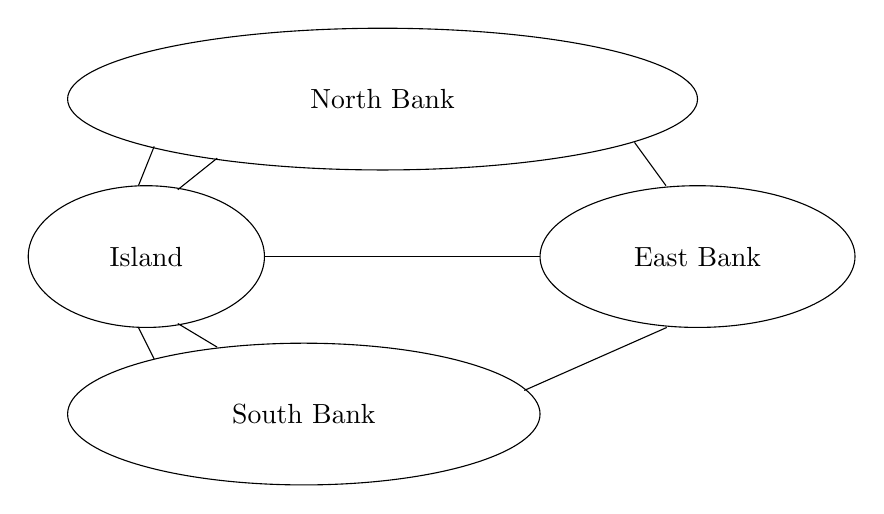
\begin{tikzpicture}
\draw (2,2) ellipse (4cm and .9cm); %NB
\node at (2,2) {North Bank};
\draw (-1,0) ellipse (1.5cm and .9cm); %I
\node at (-1,0) {Island};
\draw (6,0) ellipse (2cm and .9cm); %EB
\node at (6,0) {East Bank};
\draw (1,-2) ellipse (3cm and .9cm);
\node at (1,-2) {South Bank};
\draw(-1.1,.9)--(-.9,1.4);
\draw(-.6,.85)--(-.1,1.25);
\draw(-1.1,-.9)--(-.9,-1.3);
\draw(-.6,-.85)--(-.1,-1.15);
\draw(0.5,0)--(4,0);
\draw(5.6,0.9)--(5.2,1.45);
\draw(5.61,-0.9)--(3.8,-1.7);
\end{tikzpicture}\par\captionof{figure}{Skema empat daratan K\"onigsberg yang digambar sebagai elips berlabel (North Bank, Island, East...}\label{fig:graphtheory-dor1-tikz03}% fig-num-auto

\end{center}
Karena ukuran setiap daratan tidak relevan bagi persoalan penyeberangan jembatan, masing-masing dapat diperkecil menjadi sebuah simpul yang merepresentasikan lokasinya:
\begin{center}
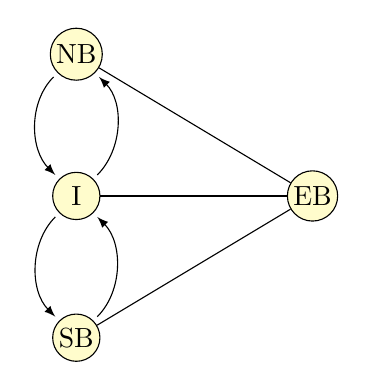
\begin{tikzpicture}[
  every node/.style={circle, draw, fill=yellow!20, minimum size=6mm, inner sep=1pt},
  >=latex
]
  % Nodes
  \node (SB) at (0,0) {SB};
  \node (I)  at (0,1.8) {I};
  \node (NB) at (0,3.6) {NB};
  \node (EB) at (3,1.8) {EB};

  % Straight edges
  \draw (SB) -- (EB);
  \draw (I)  -- (EB);
  \draw (NB) -- (EB);

  % Curved arcs with spacing from node boundaries
    \draw[->, shorten >=2pt, shorten <=2pt] (I) to[out=45, in=-45] (NB);
  \draw[->, shorten >=2pt, shorten <=2pt] (NB) to[out=225, in=135] (I);
  \draw[->, shorten >=2pt, shorten <=2pt] (SB) to[out=45, in=-45] (I);
  \draw[->, shorten >=2pt, shorten <=2pt] (I) to[out=225, in=135] (SB);

\end{tikzpicture}\par\captionof{figure}{Abstraksi graf jembatan K\"onigsberg: empat simpul bundar berlabel NB, I, EB, dan SB dengan...}\label{fig:graphtheory-dor1-tikz04}% fig-num-auto

\end{center}

Perhatikan bahwa pada graf ini terdapat \textit{dua} sisi yang menghubungkan tepi utara dan pulau, sesuai dengan dua jembatan pada gambar semula.  Bergantung pada penafsiran sisi dan simpul yang sesuai untuk suatu skenario, dua simpul dapat saja dihubungkan oleh lebih dari satu sisi.

Walaupun kita belum menjawab pertanyaan sebenarnya, yaitu apakah ada rute yang menyeberangi setiap jembatan satu kali dan kembali ke lokasi awal, graf tersebut menyediakan landasan untuk menyelidiki pertanyaan ini.
 \end{example}

\section{Definisi}
Sebelumnya kita telah mendefinisikan beberapa istilah secara longgar; sekarang kita akan merumuskannya dengan lebih tepat.

\begin{definition}{Simpul}\label{def:vertex} 
Simpul adalah sebuah titik pada graf yang dapat merepresentasikan persimpangan jalan, suatu daratan, atau lokasi umum seperti “tempat kerja” atau “sekolah”.  Simpul sering kali dihubungkan oleh sisi.  Perhatikan bahwa simpul hanya ada jika sebuah titik ditempatkan secara eksplisit, bukan setiap kali dua sisi berpotongan.  Bayangkan sebuah jalan layang di atas jalan bebas hambatan: jalan bebas hambatan dan jalan di sampingnya bersilangan, tetapi kendaraan tidak dapat berpindah dari jalan samping ke jalan bebas hambatan pada titik itu. Jadi, di sana tidak ada persimpangan dan tidak ditempatkan simpul.
\end{definition}

\begin{definition}{Sisi}
Sisi menghubungkan pasangan-pasangan simpul.  Sebuah sisi dapat merepresentasikan hubungan fisik antarlokasi, seperti jalan, atau sekadar keberadaan rute yang menghubungkan kedua lokasi, seperti penerbangan maskapai.
\end{definition}

\begin{definition}{Gelang}
Gelang adalah jenis sisi khusus yang menghubungkan sebuah simpul dengan dirinya sendiri.  Gelang jarang digunakan pada graf jaringan jalan.\\

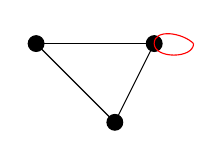
\begin{tikzpicture}
\draw[fill] (0,0) circle[radius=.1];
\draw[fill] (1,-1) circle[radius=.1];
\draw[fill] (1.5,0) circle[radius=.1];
\draw(0,0)--(1,-1);
\draw(0,0)--(1.5,0);
\draw(1.5,0)--(1,-1);  
 \draw[red](1.5,0) to [out=90] (2,0);
 \draw[red](1.5,0) to [out=-90, in=-90] (2,0);
 \end{tikzpicture}\par\captionof{figure}{Graf kecil yang mengilustrasikan sebuah gelang: tiga simpul berupa titik penuh membentuk segitiga dan sebuah gelang merah...}\label{fig:graphtheory-dor1-tikz05}% fig-num-auto

 \end{definition}

\begin{definition}{Derajat sebuah simpul}
Derajat sebuah simpul adalah banyaknya sisi yang bertemu pada simpul tersebut.  Derajat sebuah simpul dapat bernilai nol atau lebih.
\begin{center}
\begin{tabular}{|c|c|c|c|c|}
\hline
Derajat 0 & Derajat 1 & Derajat 2 & Derajat 3 & Derajat 4\\
\hline

\begin{tikzpicture}
\draw[fill] (0,0) circle[radius=.1];
\node at (0,-1){};
\end{tikzpicture}
&
\begin{tikzpicture}
\draw[fill] (0,0) circle[radius=.1];
\draw(0,0)--(1,1);
\node at (-.6,-1){};
\node at (1,1){};
\end{tikzpicture}
&
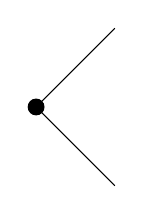
\begin{tikzpicture}
\draw[fill] (0,0) circle[radius=.1];
\draw(0,0)--(1,1);
\draw(0,0)--(1,-1);
\end{tikzpicture}
&
\begin{tikzpicture}
\draw[fill] (0,0) circle[radius=.1];
\draw(0,0)--(1,1);
\draw(0,0)--(1,-1);
\draw(0,0)--(-1,1);
\end{tikzpicture}
&
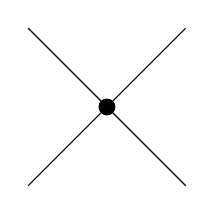
\begin{tikzpicture}
\draw[fill] (0,0) circle[radius=.1];
\draw(0,0)--(1,1);
\draw(0,0)--(1,-1);
\draw(0,0)--(-1,1);
\draw(0,0)--(-1,-1);
\end{tikzpicture}\\
\hline
\end{tabular}\par\captionof{figure}{Contoh simpul berderajat 0 sampai 4.}\label{fig:graphtheory-dor1-degrees}% fig-num-auto

\end{center}
 
 \end{definition}

\begin{definition}{Lintasan}
Lintasan adalah urutan simpul yang menggunakan sisi-sisi.  Biasanya kita tertarik pada lintasan antara dua simpul.  Sebagai contoh, sebuah lintasan dari simpul A ke simpul M diperlihatkan di bawah ini.  Lintasan tersebut merupakan salah satu dari banyak lintasan yang mungkin pada graf ini. 
\begin{center}
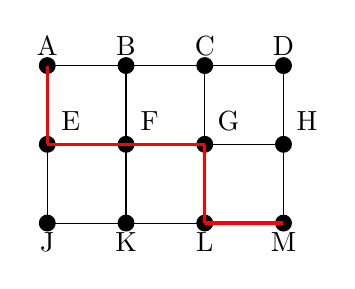
\begin{tikzpicture}
\draw[fill] (0,2) circle[radius=.1] node[above]{A};
\draw[fill] (1,2) circle[radius=.1] node[above]{B};
\draw[fill] (2,2) circle[radius=.1] node[above]{C};
\draw[fill] (3,2) circle[radius=.1] node[above]{D};
\draw[fill] (0,1) circle[radius=.1];
\node at (0.3,1.3){E}; 
\draw[fill] (1,1) circle[radius=.1];
\node at (1.3,1.3){F}; 
\draw[fill] (2,1) circle[radius=.1];
\node at (2.3,1.3){G};  
\draw[fill] (3,1) circle[radius=.1];
\node at (3.3,1.3){H};  
\draw[fill] (0,0) circle[radius=.1] node[below]{J};
\draw[fill] (1,0) circle[radius=.1] node[below]{K};
\draw[fill] (2,0) circle[radius=.1] node[below]{L};
\draw[fill] (3,0) circle[radius=.1] node[below]{M};
\draw(0,0)--(0,1);
\draw[very thick, red](0,1)--(0,2);
\draw(1,0)--(1,1);
\draw(1,1)--(1,2);
\draw[very thick, red](2,0)--(2,1);
\draw(2,1)--(2,2);
\draw(3,0)--(3,1);
\draw(3,1)--(3,2);
\draw(0,0)--(1,0);
\draw(1,0)--(2,0);
\draw[very thick, red](2,0)--(3,0);
\draw[very thick, red](0,1)--(1,1);
\draw[very thick, red](1,1)--(2,1);
\draw(2,1)--(3,1);
\draw(0,2)--(1,2);
\draw(1,2)--(2,2);
\draw(2,2)--(3,2);
\end{tikzpicture}\par\captionof{figure}{Graf kisi 3 kali 4 dengan 12 simpul berlabel A--D (atas), E--H (tengah), dan J--M (bawah).}\label{fig:graphtheory-dor1-tikz11}% fig-num-auto

\end{center}
 \end{definition}

\begin{definition}{Sirkuit (disebut juga siklus)}
Sirkuit (disebut juga siklus) adalah lintasan yang berawal dan berakhir pada simpul yang sama.  Di bawah ini diperlihatkan sebuah sirkuit (disebut juga siklus) yang berawal dan berakhir di simpul A.

\begin{center}
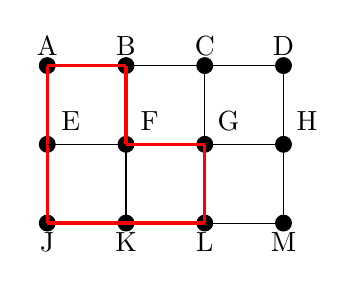
\begin{tikzpicture}
\draw[fill] (0,2) circle[radius=.1] node[above]{A};
\draw[fill] (1,2) circle[radius=.1] node[above]{B};
\draw[fill] (2,2) circle[radius=.1] node[above]{C};
\draw[fill] (3,2) circle[radius=.1] node[above]{D};
\draw[fill] (0,1) circle[radius=.1];
\node at (0.3,1.3){E}; 
\draw[fill] (1,1) circle[radius=.1];
\node at (1.3,1.3){F}; 
\draw[fill] (2,1) circle[radius=.1];
\node at (2.3,1.3){G};  
\draw[fill] (3,1) circle[radius=.1];
\node at (3.3,1.3){H};  
\draw[fill] (0,0) circle[radius=.1] node[below]{J};
\draw[fill] (1,0) circle[radius=.1] node[below]{K};
\draw[fill] (2,0) circle[radius=.1] node[below]{L};
\draw[fill] (3,0) circle[radius=.1] node[below]{M};
\draw[very thick, red](0,0)--(0,1);
\draw[very thick, red](0,1)--(0,2);
\draw(1,0)--(1,1);
\draw[very thick, red](1,1)--(1,2);
\draw[very thick, red](2,0)--(2,1);
\draw(2,1)--(2,2);
\draw(3,0)--(3,1);
\draw(3,1)--(3,2);
\draw[very thick, red](0,0)--(1,0);
\draw[very thick, red](1,0)--(2,0);
\draw(2,0)--(3,0);
\draw(0,1)--(1,1);
\draw[very thick, red](1,1)--(2,1);
\draw(2,1)--(3,1);
\draw[very thick, red](0,2)--(1,2);
\draw(1,2)--(2,2);
\draw(2,2)--(3,2);
\end{tikzpicture}\par\captionof{figure}{Graf kisi 3 kali 4 yang sama (simpul A--D, E--H, J--M) dengan sebuah sirkuit yang disorot merah tebal...}\label{fig:graphtheory-dor1-tikz12}% fig-num-auto

\end{center}
\end{definition}

\begin{definition}{Terhubung}
Sebuah graf disebut terhubung jika terdapat lintasan dari sembarang simpul ke setiap simpul lainnya.  Semua graf yang telah digambar sejauh ini merupakan graf terhubung.  Graf di bawah ini \textbf{tidak terhubung}; tidak ada cara untuk berpindah dari simpul-simpul di sebelah kiri ke simpul-simpul di sebelah kanan.

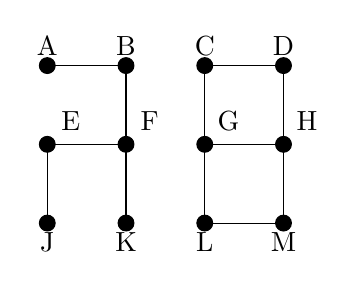
\begin{tikzpicture}
\draw[fill] (0,2) circle[radius=.1] node[above]{A};
\draw[fill] (1,2) circle[radius=.1] node[above]{B};
\draw[fill] (2,2) circle[radius=.1] node[above]{C};
\draw[fill] (3,2) circle[radius=.1] node[above]{D};
\draw[fill] (0,1) circle[radius=.1];
\node at (0.3,1.3){E}; 
\draw[fill] (1,1) circle[radius=.1];
\node at (1.3,1.3){F}; 
\draw[fill] (2,1) circle[radius=.1];
\node at (2.3,1.3){G};  
\draw[fill] (3,1) circle[radius=.1];
\node at (3.3,1.3){H};  
\draw[fill] (0,0) circle[radius=.1] node[below]{J};
\draw[fill] (1,0) circle[radius=.1] node[below]{K};
\draw[fill] (2,0) circle[radius=.1] node[below]{L};
\draw[fill] (3,0) circle[radius=.1] node[below]{M};
\draw(0,0)--(0,1);
\draw(1,0)--(1,1);
\draw(1,1)--(1,2);
\draw(2,0)--(2,1);
\draw(2,1)--(2,2);
\draw(3,0)--(3,1);
\draw(3,1)--(3,2);
\draw(2,0)--(3,0);
\draw(0,1)--(1,1);

\draw(2,1)--(3,1);
\draw(0,2)--(1,2);
\draw(2,2)--(3,2);
\end{tikzpicture}\par\captionof{figure}{Graf kisi 3 kali 4 dengan simpul A--D, E--H, J--M, tetapi sisi horizontal pada kolom A dihapus sehingga...}\label{fig:graphtheory-dor1-tikz13}% fig-num-auto

 \end{definition}

\begin{definition}{Bobot}
Bergantung pada masalah yang hendak diselesaikan, terkadang sisi-sisi diberi bobot.  Bobot dapat merepresentasikan jarak antara dua lokasi, waktu tempuh, atau biaya perjalanan.  Penting untuk diperhatikan bahwa jarak antarsimpul pada gambar graf tidak harus sesuai dengan bobot sebuah sisi.
 \end{definition}

\begin{learningcheckpoint}[label={lc:graph-5cities}]
\label{ex:5cities}
Graf di bawah ini memperlihatkan 5 kota.  Bobot pada sisi merepresentasikan harga tiket penerbangan sekali jalan antarkota.
 \begin{enumerate}[label=\alph*.]
 \item Berapa banyak simpul dan sisi yang dimiliki graf tersebut?
 \item Apakah graf tersebut terhubung?
 \item Berapakah derajat simpul yang merepresentasikan LA?
 \item Jika Anda terbang dari Seattle ke Dallas lalu ke Atlanta, apakah itu lintasan atau sirkuit?
 \item Jika Anda terbang dari LA ke Chicago lalu ke Dallas dan kembali ke LA, apakah itu lintasan atau sirkuit?
 \end{enumerate}
 
 \begin{center}
 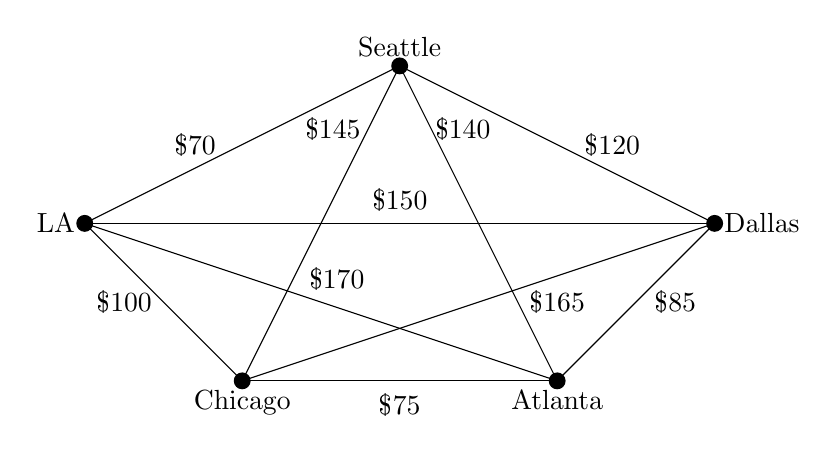
\begin{tikzpicture}
 \draw[fill] (0,0) circle[radius=.1] node[left]{LA};
\draw[fill] (2,-2) circle[radius=.1] node[below]{Chicago};
\draw[fill] (4,2) circle[radius=.1] node[above]{Seattle};
\draw[fill] (6,-2) circle[radius=.1] node[below]{Atlanta};
\draw[fill] (8,0) circle[radius=.1] node[right]{Dallas};
\draw(0,0)--(2,-2);
\node at (0.5,-1){\$100};
\draw(0,0)--(4,2);
\node at (1.4,1){\$70};
\draw(0,0)--(8,0);
\node at (4,0.3){\$150};
\draw(0,0)--(6,-2);
\node at (3.2,-0.7){\$170};
\draw(2,-2)--(4,2);
\node at (3.15,1.2){\$145};
\draw(4,2)--(6,-2);
\node at (4.8, 1.2){\$140};
\draw(4,2)--(8,0);
\node at (6.7,1){\$120};
\draw(2,-2)--(8,0);
\node at (6,-1){\$165};
\draw(2,-2)--(6,-2);
\node at (4,-2.3){\$75};
\draw(6,-2)--(8,0);
\node at (7.5,-1){\$85};
 \end{tikzpicture}\par\captionof{figure}{Graf berbobot lima kota di A.S. (LA, Seattle, Chicago, Atlanta, Dallas) yang diperlihatkan sebagai titik-titik penuh...}\label{fig:graphtheory-dor1-tikz14}% fig-num-auto

 \end{center}
 \end{learningcheckpoint}

\section{Lintasan Terpendek}
\label{sec:gt-shortest-path}
\begin{outcome}
\begin{itemize}
\item Apa rumusan masalahnya?
\item Cara menggunakan algoritme Dijkstra
\item Solusi perangkat lunak
\end{itemize}
\end{outcome}
\begin{resource}
\begin{itemize}
\item \href{https://www.youtube.com/watch?v=EFg3u_E6eHU&ab_channel=SpanningTree}{Cara kerja algoritme Dijkstra}
\item \href{https://youtu.be/EFg3u_E6eHU}{Video YouTube tentang Algoritme Dijkstra}
\item \href{https://github.com/open-optimization/open-optimization-or-book/blob/master/instructive-code/networkx%20example%20-%20Dijkstra's%20Algorithm.ipynb}{Contoh Python yang menggunakan NetworkX dan juga memperlihatkan algoritme Dijkstra}
\end{itemize}
\end{resource}
Ketika Anda mengunjungi situs seperti Google Maps atau menggunakan ponsel pintar untuk meminta petunjuk arah dari rumah ke rumah bibi Anda di Pasadena, biasanya Anda sedang mencari lintasan terpendek antara kedua lokasi tersebut.  Aplikasi komputer ini merepresentasikan peta jalan sebagai graf, dengan perkiraan waktu berkendara sebagai bobot sisi.

Walaupun lintasan terpendek pada graf kecil sering kali dapat ditemukan dengan cara menebak lalu memeriksa, tujuan kita dalam bab ini adalah mengembangkan metode untuk menyelesaikan masalah kompleks secara sistematis dengan mengikuti \textbf{algoritme}.  Algoritme adalah prosedur langkah demi langkah untuk menyelesaikan suatu masalah.  Algoritme Dijkstra (dilafalkan daik-stra) akan menemukan lintasan terpendek antara dua simpul.

\newcommand{\dijkstra}[6]{
\begin{center}
\begin{tikzpicture}[scale=1.7,
  graphNode/.style={circle, draw, fill=blue!20, minimum size=8mm, inner sep=0pt, font=\bfseries},
  aboveLabel/.style={rectangle, draw=green!60!black, fill=green!20, font=\small, minimum height=4mm},
  edgeLabel/.style={font=\small}
]

% Nodes with green boxed labels
\node[graphNode] (T) at (0,0) {T};
\node[aboveLabel, above=2pt of T] {0};

\node[graphNode] (E) at (2,-2) {E};
\node[aboveLabel, above=2pt of E] {#5};

\node[graphNode] (A) at (2,1) {A};
\node[aboveLabel, above=2pt of A] {#4};

\node[graphNode] (NB) at (4,2) {NB};
\node[aboveLabel, above=2pt of NB] {#3};

\node[graphNode] (MR) at (4,0) {MR};
\node[aboveLabel, above=2pt of MR] {#2};

\node[graphNode] (P) at (4,-1) {P};
\node[aboveLabel, below=2pt of P] {#1};

\node[graphNode] (Y) at (8,0) {Y};
\node[aboveLabel, above=2pt of Y] {#6};

% Edges with plain text labels
\draw (T) -- (E) node[midway, left, edgeLabel] {57};
\draw (T) -- (A) node[midway, left, edgeLabel] {20};
\draw (A) -- (NB) node[midway, left, edgeLabel] {36};
\draw (NB) -- (Y) node[midway, above, edgeLabel] {120};
\draw (E) -- (P) node[midway, below, edgeLabel] {27};
\draw (P) -- (Y) node[midway, below, edgeLabel] {76};
\draw (A) -- (MR) node[midway, above, edgeLabel] {79};
\draw (MR) -- (P) node[midway, left, edgeLabel] {10};
\draw (MR) -- (Y) node[midway, above, edgeLabel] {90};
\end{tikzpicture}\par\captionof{figure}{Diagram keadaan awal algoritme Dijkstra: tujuh simpul bundar biru T, E, A, NB, MR, P, Y...}\label{fig:graphtheory-dor1-tikz15}% fig-num-auto

\end{center}
}

\newcommand{\ph}{\phantom{$\infty$}}

\begin{algorithm}{Algoritme Dijkstra}{}{}
{\Large \textbf{Algoritme Dijkstra} } \\
\hspace{3in}

\begin{enumerate}
\item	Tandai simpul akhir dengan jarak nol.  Tetapkan simpul ini sebagai simpul aktif.

\dijkstra{$\infty$}{$\infty$}{$\infty$}{$\infty$}{$\infty$}{$\infty$}

\item Temukan semua simpul yang menuju simpul aktif.  Hitung jarak masing-masing ke tujuan.  Karena jarak simpul aktif ke tujuan sudah diketahui, kita hanya perlu menambahkan sisi terakhir.  Jangan catat jarak ini jika lebih panjang daripada jarak yang telah dicatat sebelumnya.
\item	Tandai simpul aktif sebagai telah dikunjungi.  Simpul ini tidak akan kita periksa lagi.
\item	Tetapkan simpul dengan jarak terkecil sebagai simpul aktif, lalu ulangi dari langkah 2.
\end{enumerate}
 \end{algorithm}

\newpage
\begin{example}{}
Misalkan Anda perlu bepergian dari Yakima, Washington (simpul Y), ke Tacoma, Washington (simpul T).  Dari peta, perjalanan melalui Auburn (A) lalu Mount Rainier (MR) tampaknya mungkin paling singkat, tetapi hal itu belum sepenuhnya jelas karena jalan tersebut mungkin lebih lambat daripada jalan raya utama melalui North Bend (NB).  Graf dengan waktu tempuh dalam menit diperlihatkan di bawah ini.  Rute alternatif melalui Eatonville (E) dan Packwood (P) juga diperlihatkan.

\begin{tikzpicture}[scale=1.7,
  graphNode/.style={circle, draw, fill=blue!20, minimum size=8mm, inner sep=0pt, font=\bfseries},
  aboveLabel/.style={rectangle, draw=green!60!black, fill=green!20, font=\small, minimum height=4mm},
  edgeLabel/.style={font=\small}
]
\draw[fill] (0,0) circle[radius=.1] node[left]{T};
\draw[fill] (2,-2) circle[radius=.1] node[left]{E};
\draw[fill] (2,1) circle[radius=.1];
\node at (1.7,1.2){A};
\draw[fill] (4,2) circle[radius=.1]; 
\node at (3.6,2.2){NB};
\draw[fill] (4,0) circle[radius=.1];
\node at (4.05,0.3){MR};
\draw[fill] (4,-1) circle[radius=.1];
\node at (4.3,-1.2){P};
\draw[fill] (8,0) circle[radius=.1] node[right]{Y};
\draw(0,0)--(2,-2);
\node at (0.6,-1){57};
\draw(0,0)--(2,1);
\node at (0.5, 0.5){20};
\draw(2,1)--(4,2);
\node at (2.5,1.5){36};
\draw(4,2)--(8,0);
\node at (6,1.3){104};
\draw(2,-2)--(4,-1);
\node at (3,-1.8){96};
\draw(4,-1)--(8,0);
\node at (6,-0.7){76};
\draw(2,1)--(4,0);
\node at (3.1,0.7){79};
\draw(4,0)--(4,-1);
\node at (3.7, -0.5){27};
\draw(4,0)--(8,0);
\node at (6,0.3){96};
\end{tikzpicture}\par\captionof{figure}{Jaringan jalan berbobot untuk contoh Yakima-ke-Tacoma: tujuh simpul berupa titik penuh T (Tacoma), E...}\label{fig:graphtheory-dor1-tikz16}% fig-num-auto


\noindent Langkah 1:  Tandai simpul akhir dengan jarak nol.  Jarak akan dicatat dalam [kurung siku] setelah nama simpul.\\
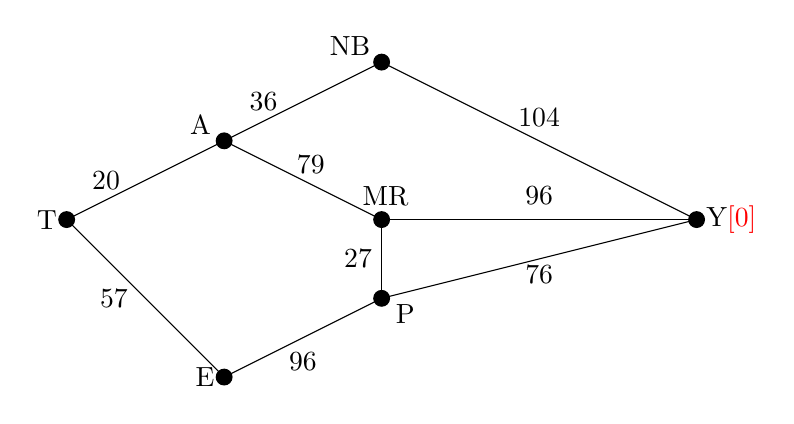
\begin{tikzpicture}
\draw[fill] (0,0) circle[radius=.1] node[left]{T};
\draw[fill] (2,-2) circle[radius=.1] node[left]{E};
\draw[fill] (2,1) circle[radius=.1];
\node at (1.7,1.2){A};
\draw[fill] (4,2) circle[radius=.1]; 
\node at (3.6,2.2){NB};
\draw[fill] (4,0) circle[radius=.1];
\node at (4.05,0.3){MR};
\draw[fill] (4,-1) circle[radius=.1];
\node at (4.3,-1.2){P};
\draw[fill] (8,0) circle[radius=.1] node[right]{Y\textcolor{red}{[0]}};
\draw(0,0)--(2,-2);
\node at (0.6,-1){57};
\draw(0,0)--(2,1);
\node at (0.5, 0.5){20};
\draw(2,1)--(4,2);
\node at (2.5,1.5){36};
\draw(4,2)--(8,0);
\node at (6,1.3){104};
\draw(2,-2)--(4,-1);
\node at (3,-1.8){96};
\draw(4,-1)--(8,0);
\node at (6,-0.7){76};
\draw(2,1)--(4,0);
\node at (3.1,0.7){79};
\draw(4,0)--(4,-1);
\node at (3.7, -0.5){27};
\draw(4,0)--(8,0);
\node at (6,0.3){96};
\end{tikzpicture}\par\captionof{figure}{Jaringan jalan Yakima-ke-Tacoma seperti sebelumnya, kini dengan tujuan Y diberi anotasi [0] berwarna merah untuk menandainya...}\label{fig:graphtheory-dor1-tikz17}% fig-num-auto


\noindent Langkah 2:  Untuk setiap simpul yang menuju Y, kita hitung jaraknya ke tujuan.  Sebagai contoh, jarak NB ke tujuan adalah 104 dan jarak MR ke tujuan adalah 96.  Ingatlah bahwa jarak dalam kasus ini mengacu pada waktu tempuh dalam menit.\\
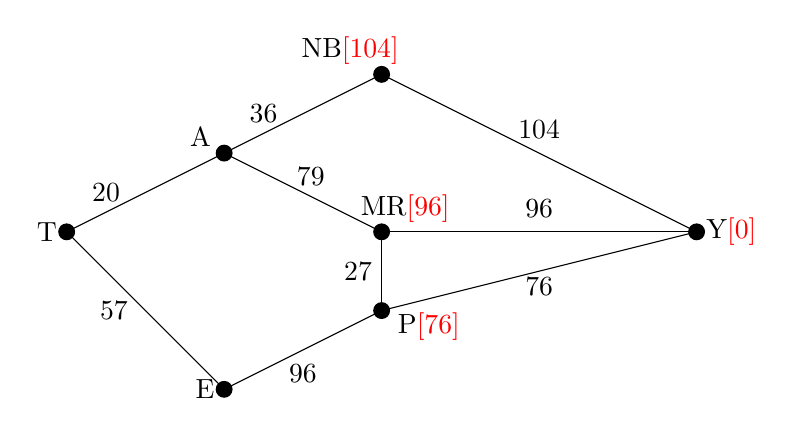
\begin{tikzpicture}
\draw[fill] (0,0) circle[radius=.1] node[left]{T};
\draw[fill] (2,-2) circle[radius=.1] node[left]{E};
\draw[fill] (2,1) circle[radius=.1];
\node at (1.7,1.2){A};
\draw[fill] (4,2) circle[radius=.1]; 
\node at (3.6,2.3){NB\textcolor{red}{[104]}};
\draw[fill] (4,0) circle[radius=.1];
\node at (4.3,0.3){MR\textcolor{red}{[96]}};
\draw[fill] (4,-1) circle[radius=.1];
\node at (4.6,-1.2){P\textcolor{red}{[76]}};
\draw[fill] (8,0) circle[radius=.1] node[right]{Y\textcolor{red}{[0]}};
\draw(0,0)--(2,-2);
\node at (0.6,-1){57};
\draw(0,0)--(2,1);
\node at (0.5, 0.5){20};
\draw(2,1)--(4,2);
\node at (2.5,1.5){36};
\draw(4,2)--(8,0);
\node at (6,1.3){104};
\draw(2,-2)--(4,-1);
\node at (3,-1.8){96};
\draw(4,-1)--(8,0);
\node at (6,-0.7){76};
\draw(2,1)--(4,0);
\node at (3.1,0.7){79};
\draw(4,0)--(4,-1);
\node at (3.7, -0.5){27};
\draw(4,0)--(8,0);
\node at (6,0.3){96};
\end{tikzpicture}\par\captionof{figure}{Contoh Yakima setelah langkah 2 Dijkstra: jarak sementara [104] di NB, [96] di MR, [76] di P...}\label{fig:graphtheory-dor1-tikz18}% fig-num-auto


\noindent Langkah 3 \& 4:  Kita tandai Y sebagai telah dikunjungi, lalu tetapkan simpul dengan jarak tercatat paling kecil sebagai simpul aktif.  Pada tahap ini, P ditetapkan sebagai simpul aktif.  Kembali ke langkah 2.\\

\newpage
\noindent Langkah 2 (\#2):  Untuk setiap simpul yang menuju P (dan tidak menuju simpul yang telah dikunjungi), kita cari jaraknya ke tujuan.  Karena jarak E ke P adalah 96 menit dan kita telah menghitung bahwa jarak P ke Y adalah 76 menit, kita dapat menghitung bahwa jarak E ke Y adalah $96+76 = 172$ menit.  \\

Jika kita melakukan perhitungan yang sama untuk MR, kita memperoleh $76+27 = 103$.  Karena nilai ini lebih besar daripada jarak Y ke MR yang telah dicatat sebelumnya, kita tidak menggantinya.\\
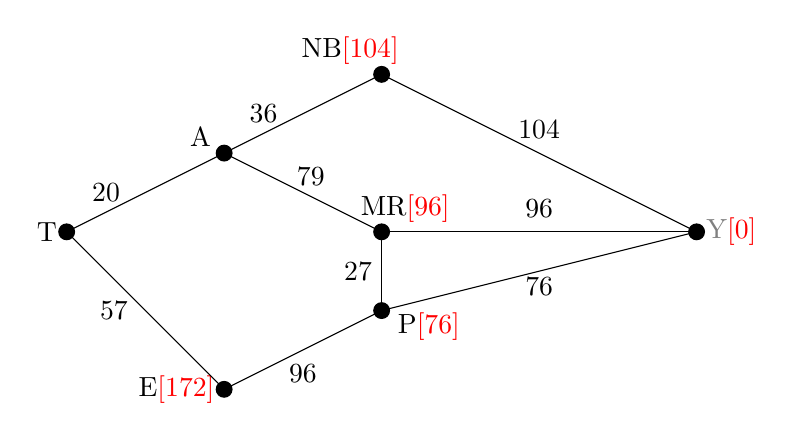
\begin{tikzpicture}
\draw[fill] (0,0) circle[radius=.1] node[left]{T};
\draw[fill] (2,-2) circle[radius=.1] node[left]{E\textcolor{red}{[172]}};
\draw[fill] (2,1) circle[radius=.1];
\node at (1.7,1.2){A};
\draw[fill] (4,2) circle[radius=.1]; 
\node at (3.6,2.3){NB\textcolor{red}{[104]}};
\draw[fill] (4,0) circle[radius=.1];
\node at (4.3,0.3){MR\textcolor{red}{[96]}};
\draw[fill] (4,-1) circle[radius=.1];
\node at (4.6,-1.2){P\textcolor{red}{[76]}};
\draw[fill] (8,0) circle[radius=.1] node[right]{\textcolor{gray}{\sout{Y}}\textcolor{red}{[0]}};
\draw(0,0)--(2,-2);
\node at (0.6,-1){57};
\draw(0,0)--(2,1);
\node at (0.5, 0.5){20};
\draw(2,1)--(4,2);
\node at (2.5,1.5){36};
\draw(4,2)--(8,0);
\node at (6,1.3){104};
\draw(2,-2)--(4,-1);
\node at (3,-1.8){96};
\draw(4,-1)--(8,0);
\node at (6,-0.7){76};
\draw(2,1)--(4,0);
\node at (3.1,0.7){79};
\draw(4,0)--(4,-1);
\node at (3.7, -0.5){27};
\draw(4,0)--(8,0);
\node at (6,0.3){96};
\end{tikzpicture}\par\captionof{figure}{Contoh Yakima setelah iterasi kedua: P merupakan simpul aktif; E kini memiliki jarak sementara...}\label{fig:graphtheory-dor1-tikz19}% fig-num-auto


\noindent Langkah 3 \& 4 (\#2):  Kita tandai P sebagai telah dikunjungi dan tetapkan simpul dengan jarak tercatat paling kecil sebagai simpul aktif, yaitu MR.  Kembali ke langkah 2.\\

\noindent Langkah 2 (\#3):  Untuk setiap simpul yang menuju MR (dan tidak menuju simpul yang telah dikunjungi), kita cari jaraknya ke tujuan.  Satu-satunya simpul yang perlu dipertimbangkan adalah A karena Y dan P telah dikunjungi.  Dengan menambahkan jarak MR sebesar 96 pada jarak A ke MR, kita memperoleh jarak A ke Y sebesar $96+79 = 175$ menit.  \\
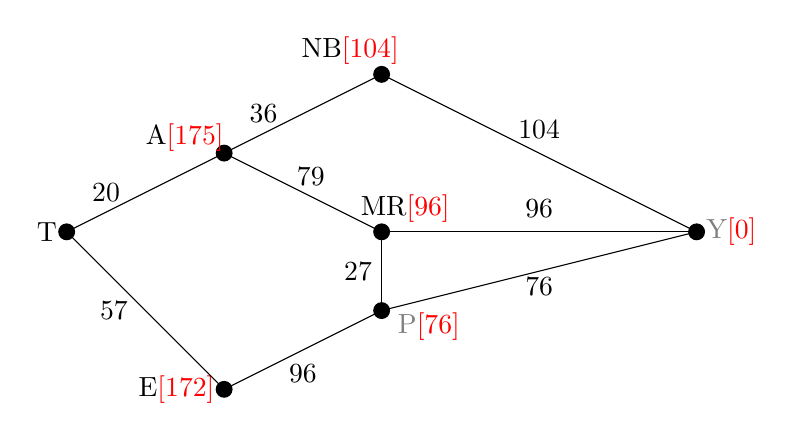
\begin{tikzpicture}
\draw[fill] (0,0) circle[radius=.1] node[left]{T};
\draw[fill] (2,-2) circle[radius=.1] node[left]{E\textcolor{red}{[172]}};
\draw[fill] (2,1) circle[radius=.1];
\node at (1.5,1.2){A\textcolor{red}{[175]}};
\draw[fill] (4,2) circle[radius=.1]; 
\node at (3.6,2.3){NB\textcolor{red}{[104]}};
\draw[fill] (4,0) circle[radius=.1];
\node at (4.3,0.3){MR\textcolor{red}{[96]}};
\draw[fill] (4,-1) circle[radius=.1];
\node at (4.6,-1.2){\textcolor{gray}{\sout{P}}\textcolor{red}{[76]}};
\draw[fill] (8,0) circle[radius=.1] node[right]{\textcolor{gray}{\sout{Y}}\textcolor{red}{[0]}};
\draw(0,0)--(2,-2);
\node at (0.6,-1){57};
\draw(0,0)--(2,1);
\node at (0.5, 0.5){20};
\draw(2,1)--(4,2);
\node at (2.5,1.5){36};
\draw(4,2)--(8,0);
\node at (6,1.3){104};
\draw(2,-2)--(4,-1);
\node at (3,-1.8){96};
\draw(4,-1)--(8,0);
\node at (6,-0.7){76};
\draw(2,1)--(4,0);
\node at (3.1,0.7){79};
\draw(4,0)--(4,-1);
\node at (3.7, -0.5){27};
\draw(4,0)--(8,0);
\node at (6,0.3){96};
\end{tikzpicture}\par\captionof{figure}{Contoh Yakima setelah iterasi ketiga: A memiliki jarak sementara [175] (melalui MR); P dan Y tampak...}\label{fig:graphtheory-dor1-tikz20}% fig-num-auto


\noindent Langkah 3 \& 4 (\#3):  Kita tandai MR sebagai telah dikunjungi dan tetapkan simpul dengan jarak tercatat paling kecil sebagai simpul aktif, yaitu NB.  Kembali ke langkah 2.\\

\noindent Langkah 2 (\#4):  Untuk setiap simpul yang menuju NB, kita cari jaraknya ke tujuan.  Kita tahu bahwa jarak terpendek dari NB ke Y adalah 104 dan jarak dari A ke NB adalah 36, sehingga jarak dari A ke Y melalui NB adalah $104+36 = 140$.  Karena jarak ini lebih pendek daripada jarak Y ke A melalui MR yang dihitung sebelumnya, kita menggantinya.\\
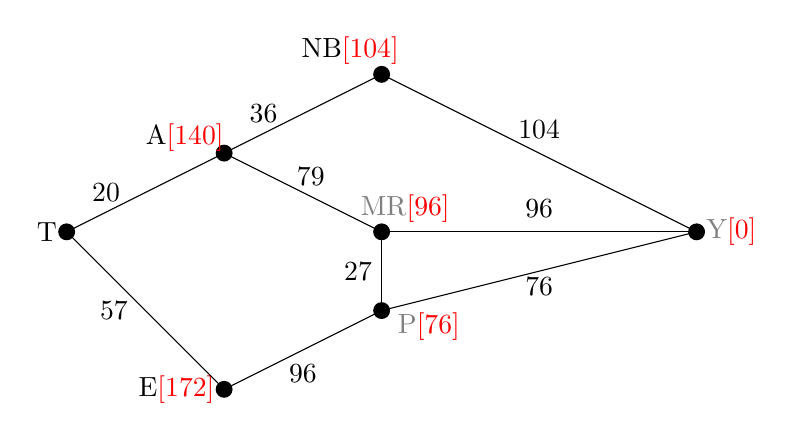
\begin{tikzpicture}
\draw[fill] (0,0) circle[radius=.1] node[left]{T};
\draw[fill] (2,-2) circle[radius=.1] node[left]{E\textcolor{red}{[172]}};
\draw[fill] (2,1) circle[radius=.1];
\node at (1.5,1.2){A\textcolor{red}{[140]}};
\draw[fill] (4,2) circle[radius=.1]; 
\node at (3.6,2.3){NB\textcolor{red}{[104]}};
\draw[fill] (4,0) circle[radius=.1];
\node at (4.3,0.3){\textcolor{gray}{\sout{MR}}\textcolor{red}{[96]}};
\draw[fill] (4,-1) circle[radius=.1];
\node at (4.6,-1.2){\textcolor{gray}{\sout{P}}\textcolor{red}{[76]}};
\draw[fill] (8,0) circle[radius=.1] node[right]{\textcolor{gray}{\sout{Y}}\textcolor{red}{[0]}};
\draw(0,0)--(2,-2);
\node at (0.6,-1){57};
\draw(0,0)--(2,1);
\node at (0.5, 0.5){20};
\draw(2,1)--(4,2);
\node at (2.5,1.5){36};
\draw(4,2)--(8,0);
\node at (6,1.3){104};
\draw(2,-2)--(4,-1);
\node at (3,-1.8){96};
\draw(4,-1)--(8,0);
\node at (6,-0.7){76};
\draw(2,1)--(4,0);
\node at (3.1,0.7){79};
\draw(4,0)--(4,-1);
\node at (3.7, -0.5){27};
\draw(4,0)--(8,0);
\node at (6,0.3){96};
\end{tikzpicture}\par\captionof{figure}{Contoh Yakima setelah iterasi keempat: jarak A diperbarui menjadi [140] melalui NB; NB, MR, P, Y...}\label{fig:graphtheory-dor1-tikz21}% fig-num-auto


\noindent Langkah 3 \& 4 (\#4):  Kita tandai NB sebagai telah dikunjungi dan tetapkan A sebagai simpul aktif karena kini A memiliki jarak terpendek.\\

\noindent Langkah 2 (\#5):  T adalah satu-satunya simpul yang belum dikunjungi dan menuju A, sehingga kita hitung jarak dari T ke Y melalui A: $20+140 = 160$ menit.  \\
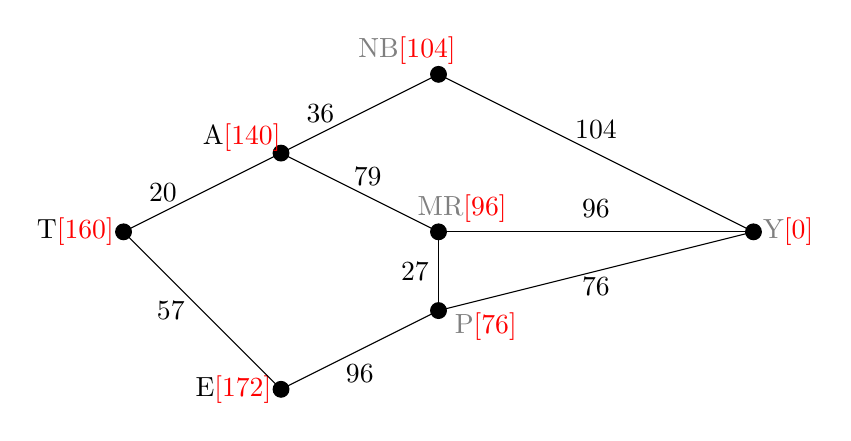
\begin{tikzpicture}
\draw[fill] (0,0) circle[radius=.1] node[left]{T\textcolor{red}{[160]}};
\draw[fill] (2,-2) circle[radius=.1] node[left]{E\textcolor{red}{[172]}};
\draw[fill] (2,1) circle[radius=.1];
\node at (1.5,1.2){A\textcolor{red}{[140]}};
\draw[fill] (4,2) circle[radius=.1]; 
\node at (3.6,2.3){\textcolor{gray}{\sout{NB}}\textcolor{red}{[104]}};
\draw[fill] (4,0) circle[radius=.1];
\node at (4.3,0.3){\textcolor{gray}{\sout{MR}}\textcolor{red}{[96]}};
\draw[fill] (4,-1) circle[radius=.1];
\node at (4.6,-1.2){\textcolor{gray}{\sout{P}}\textcolor{red}{[76]}};
\draw[fill] (8,0) circle[radius=.1] node[right]{\textcolor{gray}{\sout{Y}}\textcolor{red}{[0]}};
\draw(0,0)--(2,-2);
\node at (0.6,-1){57};
\draw(0,0)--(2,1);
\node at (0.5, 0.5){20};
\draw(2,1)--(4,2);
\node at (2.5,1.5){36};
\draw(4,2)--(8,0);
\node at (6,1.3){104};
\draw(2,-2)--(4,-1);
\node at (3,-1.8){96};
\draw(4,-1)--(8,0);
\node at (6,-0.7){76};
\draw(2,1)--(4,0);
\node at (3.1,0.7){79};
\draw(4,0)--(4,-1);
\node at (3.7, -0.5){27};
\draw(4,0)--(8,0);
\node at (6,0.3){96};
\end{tikzpicture}\par\captionof{figure}{Contoh Yakima setelah iterasi kelima: T menerima jarak sementara [160] melalui A; A, NB, MR, P...}\label{fig:graphtheory-dor1-tikz22}% fig-num-auto


\noindent Langkah 3 \& 4 (\#5):  Kita tandai A sebagai telah dikunjungi dan tetapkan E sebagai simpul aktif.\\

\noindent Langkah 2 (\#6):  Satu-satunya simpul yang belum dikunjungi dan menuju E adalah T.  Dengan menghitung jarak dari T ke Y melalui E, kita memperoleh $172+57 = 229$ menit.  Karena nilai ini lebih panjang daripada waktu yang telah ditandai, kita tidak menggantinya.  \\

\noindent Langkah 3 (\#6):  Kita tandai E sebagai telah dikunjungi.  Karena semua simpul telah dikunjungi, proses selesai.  \\

Dari hasil ini, kita mengetahui bahwa lintasan terpendek dari Yakima ke Tacoma memerlukan waktu 160 menit.  Dengan menelusuri urutan sisi yang menghasilkan 160 menit, kita melihat bahwa lintasan terpendeknya adalah Y-NB-A-T. 
\end{example}

Algoritme Dijkstra merupakan \textbf{algoritme optimal}, artinya algoritme ini selalu menghasilkan lintasan yang benar-benar terpendek, bukan sekadar lintasan yang cukup pendek, asalkan lintasan tersebut ada.  Algoritme ini juga \textbf{efisien}, artinya dapat diimplementasikan dalam waktu yang wajar.  Algoritme Dijkstra memerlukan sekitar V$^2$ perhitungan, dengan V menyatakan banyaknya simpul pada graf\footnote{Algoritme ini dapat dijalankan lebih cepat melalui berbagai pengoptimalan implementasi.}.  Graf dengan 100 simpul akan memerlukan sekitar 10.000 perhitungan.  Walaupun jumlah itu sangat banyak jika dikerjakan dengan tangan, komputer dapat menanganinya dengan mudah.  Karena efisiensi inilah perangkat GPS mobil Anda dapat menghitung petunjuk arah hanya dalam beberapa detik.  
 
Sebaliknya, algoritme yang \textbf{tidak efisien} mungkin mencoba mendaftar semua lintasan yang mungkin lalu menghitung panjang setiap lintasan.  Upaya mendaftar semua lintasan yang mungkin dapat dengan mudah memerlukan 10$^{25}$ perhitungan untuk mencari lintasan terpendek pada graf yang hanya memiliki 25 simpul; bilangan itu adalah angka 1 yang diikuti 25 nol!  Sebagai gambaran, komputer tercepat di dunia pun masih akan memerlukan lebih dari 1.000 tahun untuk menganalisis semua lintasan tersebut.

\begin{example}{Contoh algoritme Dijkstra}
Kita ingin menemukan lintasan terpendek pada graf dari simpul a ke simpul g.  Lihat \href{https://github.com/open-optimization/open-optimization-or-book/blob/master/instructive-code/networkx%20example%20-%20Dijkstra's%20Algorithm.ipynb}{Kode}
untuk kode Python yang menyelesaikan masalah ini dan membuat gambar-gambar berikut.\\
\begin{center}
\altincludegraphics[scale = 0.5]{graph-theory-graphics/dijkstra0.png}{Graf tak berarah berbobot untuk contoh Dijkstra. Tujuh simpul a--g dihubungkan oleh sisi berbobot a-b=2, a-c=6, c-d=8, b-d=5, d-e=10, d-f=15, e-f=6, e-g=2, f-g=6. Belum ada simpul yang ditandai sebagai telah dikunjungi.}\\\par\captionof{figure}{Graf tak berarah berbobot untuk contoh Dijkstra.}\label{fig:dijkstra0}% fig-num-auto

\end{center}
Kita akan menginisialisasi algoritme pada simpul 'a'.  

\begin{minipage}{0.49\textwidth}
\altincludegraphics[scale = 0.5]{graph-theory-graphics/dijkstra1.png}{Langkah 1 Dijkstra: simpul awal a disorot merah dan diberi label jarak sementara 0. Tetangganya, b dan c, menerima label sementara 2 dan 6 dari a; semua simpul lain tetap berlabel tak hingga.}\par\captionof{figure}{Langkah 1 Dijkstra: simpul awal a disorot merah dan diberi label jarak sementara 0.}\label{fig:dijkstra1}% fig-num-auto

\end{minipage}
\begin{minipage}{0.49\textwidth}
         \begin{tabular}{|l|l|l|l|l|l|l|l|}
    \hline
        aktif & a & b & c & d & e & f & g \\ \hline
        a & 0 & 2 & 6 & $\infty$ & $\infty$ & $\infty$& $\infty$  \\ \hline
    \end{tabular} 
    \end{minipage}\\
\begin{minipage}{0.49\textwidth}
\altincludegraphics[scale = 0.5]{graph-theory-graphics/dijkstra2.png}{Langkah 2 Dijkstra: simpul b kini ditandai telah dikunjungi dengan jarak permanen 2 dan sisi a-b disorot merah. Simpul d diperbarui melalui b menjadi berjarak sementara 7. Label pada c, e, f, dan g tidak berubah.}\par\captionof{figure}{Langkah 2 Dijkstra: simpul b kini ditandai telah dikunjungi dengan jarak permanen 2 dan sisi a-b...}\label{fig:dijkstra2}% fig-num-auto

\end{minipage}
\begin{minipage}{0.49\textwidth}
         \begin{tabular}{|l|l|l|l|l|l|l|l|}
    \hline
        aktif & a & b & c & d & e & f & g \\ \hline
        b & 0 & 2 & 6 & 7 & $\infty$ & $\infty$ & $\infty$ \\ \hline
    \end{tabular}
     \end{minipage}\\
\begin{minipage}{0.49\textwidth}
\altincludegraphics[scale = 0.5]{graph-theory-graphics/dijkstra3.png}{Langkah 3 Dijkstra: simpul c ditandai telah dikunjungi dengan jarak 6 dan sisi a-c disorot. Mencapai d melalui c akan menghasilkan 6+8=14, yang lebih buruk daripada label saat ini, yaitu 7, sehingga jarak sementara d tidak berubah.}\par\captionof{figure}{Langkah 3 Dijkstra: simpul c ditandai telah dikunjungi dengan jarak 6 dan sisi a-c disorot.}\label{fig:dijkstra3}% fig-num-auto

\end{minipage}
\begin{minipage}{0.49\textwidth}
          \begin{tabular}{|l|l|l|l|l|l|l|l|}
    \hline
        aktif & a & b & c & d & e & f & g \\ \hline
        c & 0 & 2 & 6 & 7 & $\infty$ & $\infty$ & $\infty$  \\ \hline
    \end{tabular}
     \end{minipage}\\
\begin{minipage}{0.49\textwidth}
\altincludegraphics[scale = 0.5]{graph-theory-graphics/dijkstra4.png}{Langkah 4 Dijkstra: simpul d ditandai telah dikunjungi dengan jarak 7 dan lintasan a-b-d disorot merah. Tetangga d diperbarui: e menjadi 17 (melalui 7+10) dan f menjadi 22 (melalui 7+15); g tetap tak hingga.}\par\captionof{figure}{Langkah 4 Dijkstra: simpul d ditandai telah dikunjungi dengan jarak 7 dan lintasan a-b-d disorot merah.}\label{fig:dijkstra4}% fig-num-auto
 
\end{minipage}
\begin{minipage}{0.49\textwidth}
          \begin{tabular}{|l|l|l|l|l|l|l|l|}
    \hline
        aktif & a & b & c & d & e & f & g \\ \hline
        d & 0 & 2 & 6 & 7 & 17 & 22 & $\infty$ \\ \hline
    \end{tabular}
     \end{minipage}\\
\begin{minipage}{0.49\textwidth}
\altincludegraphics[scale = 0.5]{graph-theory-graphics/dijkstra5.png}{Langkah 5 Dijkstra: simpul e ditandai telah dikunjungi dengan jarak 17 dan sisi d-e ditambahkan ke lintasan yang disorot. Dari e, simpul g diperbarui menjadi 17+2=19, lebih baik daripada label tak hingganya sebelumnya.}\par\captionof{figure}{Langkah 5 Dijkstra: simpul e ditandai telah dikunjungi dengan jarak 17 dan sisi d-e ditambahkan ke...}\label{fig:dijkstra5}% fig-num-auto

\end{minipage}
\begin{minipage}{0.49\textwidth}
         \begin{tabular}{|l|l|l|l|l|l|l|l|}
    \hline
        aktif & a & b & c & d & e & f & g \\ \hline
        e & 0 & 2 & 6 & 7 & 17 & 22 & 19 \\ \hline
    \end{tabular}
     \end{minipage}\\
\begin{minipage}{0.49\textwidth}
\altincludegraphics[scale = 0.5]{graph-theory-graphics/dijkstra6.png}{Langkah 6 Dijkstra: simpul g ditandai telah dikunjungi dengan jarak 19 dan sisi e-g disorot, melengkapi lintasan terpendek sementara a-b-d-e-g. Simpul f yang belum dikunjungi tetap memiliki jarak sementara 22.}\par\captionof{figure}{Langkah 6 Dijkstra: simpul g ditandai telah dikunjungi dengan jarak 19 dan sisi e-g disorot...}\label{fig:dijkstra6}% fig-num-auto

\end{minipage}
\begin{minipage}{0.49\textwidth}
          \begin{tabular}{|l|l|l|l|l|l|l|l|}
    \hline
        aktif & a & b & c & d & e & f & g \\ \hline
        g & 0 & 2 & 6 & 7 & 17 & 22 & 19  \\ \hline
    \end{tabular}
     \end{minipage}\\
\begin{minipage}{0.49\textwidth}
\altincludegraphics[scale = 0.5]{graph-theory-graphics/dijkstra7.png}{Langkah 7 Dijkstra: simpul f ditandai telah dikunjungi dengan jarak 22 dan sisi d-f disorot bersama lintasan yang ditemukan sebelumnya. Ketujuh simpul kini telah dikunjungi sehingga algoritme berhenti.}\par\captionof{figure}{Langkah 7 Dijkstra: simpul f ditandai telah dikunjungi dengan jarak 22 dan sisi d-f disorot bersama...}\label{fig:dijkstra7}% fig-num-auto
 
\end{minipage}
\begin{minipage}{0.49\textwidth}
 \begin{tabular}{|l|l|l|l|l|l|l|l|}
    \hline
        aktif & a & b & c & d & e & f & g \\ \hline
        f & 0 & 2 & 6 & 7 & 17 & 22 & 19  \\ \hline
    \end{tabular}
\end{minipage}\\

Sekarang kita dapat merangkum perhitungan yang mengikuti algoritme Dijkstra.\\

\begin{minipage}{0.49\textwidth}
\altincludegraphics[scale = 0.5]{graph-theory-graphics/dijkstra8.png}{Keadaan akhir contoh Dijkstra: setiap simpul memuat jarak lintasan terpendeknya dari a (a=0, b=2, c=6, d=7, e=17, g=19, f=22), dan pohon lintasan terpendek yang ditemukan algoritme disorot merah.}\par\captionof{figure}{Keadaan akhir contoh Dijkstra: setiap simpul memuat jarak lintasan terpendeknya dari a (a=0...}\label{fig:dijkstra8}% fig-num-auto
 
\end{minipage}
\begin{minipage}{0.49\textwidth}
 \begin{tabular}{|l|l|l|l|l|l|l|l|}
    \hline
        aktif & a & b & c & d & e & f & g \\ \hline
        a & 0 & 2 & 6 & $\infty$ & $\infty$ & $\infty$& $\infty$  \\ \hline
        b & 0 & 2 & 6 & 7 & $\infty$ & $\infty$ & $\infty$ \\ \hline
        c & 0 & 2 & 6 & 7 & $\infty$ & $\infty$ & $\infty$  \\ \hline
        d & 0 & 2 & 6 & 7 & 17 & 22 & $\infty$ \\ \hline
        e & 0 & 2 & 6 & 7 & 17 & 22 & 19 \\ \hline
        g & 0 & 2 & 6 & 7 & 17 & 22 & 19  \\ \hline
        f & 0 & 2 & 6 & 7 & 17 & 22 & 19  \\ \hline
    \end{tabular}
\end{minipage}\\

\paragraph{Solusi akhir} 
Lintasan terpendek dari a ke g adalah lintasan a - b - d - e - g, 
\begin{center}
\altincludegraphics[scale = 0.5]{graph-theory-graphics/dijkstra-soln.png}{Graf berbobot tujuh simpul yang sama dengan lintasan terpendek dari a ke g disorot merah: a-b-d-e-g, melewati sisi berbobot 2, 5, 10, dan 2 dengan panjang total 19.}\par\captionof{figure}{Graf berbobot tujuh simpul yang sama dengan lintasan terpendek dari a ke g disorot merah...}\label{fig:dijkstra-soln}% fig-num-auto

\end{center} 
dan memiliki panjang 
$$
2 + 5 + 10 + 2 = 19.
$$
\end{example}

\newpage
\newpage

\begin{example}{}
Sebuah perusahaan pengiriman perlu merutekan paket dari Washington, D.C., ke San Diego, California.  Untuk meminimalkan biaya, paket tersebut mula-mula dikirim ke pusat pemrosesan mereka di Baltimore, Maryland, lalu disertakan dalam pengiriman massal di antara berbagai pusat pemrosesan sampai tiba di pusat pemrosesan mereka di Bakersfield, California.  Dari sana, paket akan dikirim dengan truk kecil ke San Diego.  

Waktu tempuh dalam jam di antara pusat-pusat pemrosesan mereka diperlihatkan pada tabel di bawah ini.  Tiga jam telah ditambahkan ke setiap waktu tempuh untuk pemrosesan.  Temukan lintasan terpendek dari Baltimore ke Bakersfield.
 \begin{center}
 \begin{tabular}{|l|c|c|c|c|c|c|}
 \hline
 & Baltimore & Denver & Dallas & Chicago & Atlanta & Bakersfield\\
 &&&&&&\\
 \hline
 Baltimore & * &&&15&14&\\
 \hline
 Denver &&*&&18&24&19\\
 \hline
Dallas&&&*&18&15&25\\
 \hline
 Chicago &15&18&18&*&14&\\
 \hline
 Atlanta & 14 & 24&15&14&*&\\
 \hline
 Bakersfield &&19&25&&&*\\
 \hline
 \end{tabular}
\par\captionof{table}{Waktu tempuh dalam jam antarpusat pemrosesan, dengan tambahan tiga jam untuk pemrosesan.}\label{tab:graphtheory-dor1-tab01}% tab-num-auto

 \end{center}

Walaupun kita dapat menggambar graf, kita juga dapat bekerja langsung dari tabel. \\

\noindent Langkah 1:  Simpul akhir, Bakersfield, ditandai sebagai simpul aktif.\\

\noindent Langkah 2:  Jarak semua kota yang terhubung ke Bakersfield, dalam hal ini Denver dan Dallas, dihitung; kita akan menandai jarak tersebut pada kepala kolom.  \\

\noindent Langkah 3 \& 4:  Tandai Bakersfield sebagai telah dikunjungi.  Di sini, kita melakukannya dengan memberi bayangan pada baris dan kolom tabel yang bersesuaian.  Kita tandai Denver sebagai simpul aktif, yang ditampilkan dengan huruf tebal, karena Denver merupakan simpul dengan jarak terpendek.
 \begin{center}
 \begin{tabular}{|l|c|c|c|c|c|c|}
 \hline
 & Baltimore & \textbf{Denver} & Dallas & Chicago & Atlanta & \cellcolor{yellow}Bakersfield\\
 &&[19]&[25]&&&\cellcolor{yellow}[0]\\
 \hline
 Baltimore & * &&&15&14&\cellcolor{yellow}\\
 \hline
 Denver &&*&&18&24&\cellcolor{yellow}19\\
 \hline
Dallas&&&*&18&15&\cellcolor{yellow}25\\
 \hline
 Chicago &15&18&18&*&14&\cellcolor{yellow}\\
 \hline
 Atlanta & 14 & 24&15&14&*&\cellcolor{yellow}\\
 \hline
 \cellcolor{yellow}Bakersfield &\cellcolor{yellow}&\cellcolor{yellow}19&\cellcolor{yellow}25&\cellcolor{yellow}&\cellcolor{yellow}&\cellcolor{yellow}*\\
 \hline
 \end{tabular}
 \end{center}

\noindent Langkah 2 (\#2):  Untuk kota-kota yang terhubung ke Denver, hitung jaraknya ke tujuan.  Sebagai contoh, Chicago berjarak 18 jam dari Denver dan Denver berjarak 19 jam dari tujuan, sehingga jarak Chicago ke tujuan adalah $18+19 = 37$ (Chicago ke Denver ke Bakersfield).  Atlanta berjarak 24 jam dari Denver, sehingga jaraknya ke tujuan adalah $24+19 = 43$ (Atlanta ke Denver ke Bakersfield).\\

\noindent Langkah 3 \& 4 (\#2):  Kita tandai Denver sebagai telah dikunjungi dan Dallas sebagai simpul aktif.
 \begin{center}
 \begin{tabular}{|l|c|c|c|c|c|c|}
 \hline
 & Baltimore & \cellcolor{yellow}Denver & \textbf{Dallas} & Chicago & Atlanta & \cellcolor{yellow}Bakersfield\\
 && \cellcolor{yellow}[19]&[25]&[37]&[43]&\cellcolor{yellow}[0]\\
 \hline
 Baltimore & * & \cellcolor{yellow}&&15&14&\cellcolor{yellow}\\
 \hline
  \cellcolor{yellow}Denver & \cellcolor{yellow}& \cellcolor{yellow}*& \cellcolor{yellow}& \cellcolor{yellow}18& \cellcolor{yellow}24&\cellcolor{yellow}19\\
 \hline
Dallas&& \cellcolor{yellow}&*&18&15&\cellcolor{yellow}25\\
 \hline
 Chicago &15& \cellcolor{yellow}18&18&*&14&\cellcolor{yellow}\\
 \hline
 Atlanta & 14 &  \cellcolor{yellow}24&15&14&*&\cellcolor{yellow}\\
 \hline
 \cellcolor{yellow}Bakersfield &\cellcolor{yellow}&\cellcolor{yellow}19&\cellcolor{yellow}25&\cellcolor{yellow}&\cellcolor{yellow}&\cellcolor{yellow}*\\
 \hline
 \end{tabular}
 \end{center}

\noindent Langkah 2 (\#3):  Untuk kota-kota yang terhubung ke Dallas, hitung jaraknya ke tujuan.  Untuk Chicago, jarak Chicago ke Dallas adalah 18 dan jarak Dallas ke tujuan adalah 25, sehingga jarak Chicago ke tujuan melalui Dallas adalah $18+25 = 43$.  Karena nilai ini lebih panjang daripada jarak Chicago yang kini ditandai, kita tidak menggantinya.  Untuk Atlanta, kita hitung $15+25 = 40$.  Karena nilai ini lebih pendek daripada jarak Atlanta yang kini ditandai, kita mengganti jarak yang ada.\\

\noindent Langkah 3 \& 4 (\#3):  Kita tandai Dallas sebagai telah dikunjungi dan Chicago sebagai simpul aktif.

 \begin{center}
 \begin{tabular}{|l|c|c|c|c|c|c|}
 \hline
 & Baltimore & \cellcolor{yellow}Denver &  \cellcolor{yellow}Dallas & \textbf{Chicago} & Atlanta & \cellcolor{yellow}Bakersfield\\
 && \cellcolor{yellow}[19]& \cellcolor{yellow}[25]&[37]&[40]&\cellcolor{yellow}[0]\\
 \hline
 Baltimore & * & \cellcolor{yellow}& \cellcolor{yellow}&15&14&\cellcolor{yellow}\\
 \hline
 \cellcolor{yellow} Denver & \cellcolor{yellow}& \cellcolor{yellow}*& \cellcolor{yellow}& \cellcolor{yellow}18& \cellcolor{yellow}24&\cellcolor{yellow}19\\
 \hline
 \cellcolor{yellow}Dallas& \cellcolor{yellow}& \cellcolor{yellow}& \cellcolor{yellow}*& \cellcolor{yellow}18& \cellcolor{yellow}15&\cellcolor{yellow}25\\
 \hline
 Chicago &15& \cellcolor{yellow}18& \cellcolor{yellow}18&*&14&\cellcolor{yellow}\\
 \hline
 Atlanta & 14 &  \cellcolor{yellow}24& \cellcolor{yellow}15&14&*&\cellcolor{yellow}\\
 \hline
 \cellcolor{yellow}Bakersfield &\cellcolor{yellow}&\cellcolor{yellow}19&\cellcolor{yellow}25&\cellcolor{yellow}&\cellcolor{yellow}&\cellcolor{yellow}*\\
 \hline
 \end{tabular}
 \end{center}

\noindent Langkah 2 (\#4):  Baltimore dan Atlanta merupakan satu-satunya kota yang belum dikunjungi dan terhubung ke Chicago.  Untuk Baltimore, kita hitung 15+37 = 52 dan tandai jarak tersebut.  Untuk Atlanta, kita hitung $14+37 = 51$.  Karena nilai ini lebih panjang daripada jarak Atlanta yang ada, yaitu 40, kita tidak mengganti jarak tersebut.\\

\noindent Langkah 3 \& 4 (\#4):  Tandai Chicago sebagai telah dikunjungi dan Atlanta sebagai simpul aktif.

 \begin{center}
 \begin{tabular}{|l|c|c|c|c|c|c|}
 \hline
 & Baltimore & \cellcolor{yellow}Denver &  \cellcolor{yellow}Dallas &  \cellcolor{yellow}Chicago & \textbf{Atlanta} & \cellcolor{yellow}Bakersfield\\
 &[52]& \cellcolor{yellow}[19]& \cellcolor{yellow}[25]& \cellcolor{yellow}[37]&[40]&\cellcolor{yellow}[0]\\
 \hline
 Baltimore & * & \cellcolor{yellow}& \cellcolor{yellow}& \cellcolor{yellow}15&14&\cellcolor{yellow}\\
 \hline
 \cellcolor{yellow} Denver & \cellcolor{yellow}& \cellcolor{yellow}*& \cellcolor{yellow}& \cellcolor{yellow}18& \cellcolor{yellow}24&\cellcolor{yellow}19\\
 \hline
 \cellcolor{yellow}Dallas& \cellcolor{yellow}& \cellcolor{yellow}& \cellcolor{yellow}*& \cellcolor{yellow}18& \cellcolor{yellow}15&\cellcolor{yellow}25\\
 \hline
  \cellcolor{yellow}Chicago & \cellcolor{yellow}15& \cellcolor{yellow}18& \cellcolor{yellow}18& \cellcolor{yellow}*& \cellcolor{yellow}14&\cellcolor{yellow}\\
 \hline
 Atlanta & 14 &  \cellcolor{yellow}24& \cellcolor{yellow}15& \cellcolor{yellow}14&*&\cellcolor{yellow}\\
 \hline
 \cellcolor{yellow}Bakersfield &\cellcolor{yellow}&\cellcolor{yellow}19&\cellcolor{yellow}25&\cellcolor{yellow}&\cellcolor{yellow}&\cellcolor{yellow}*\\
 \hline
 \end{tabular}
 \end{center}

\noindent Langkah 2 (\#5):  Jarak Atlanta ke Baltimore adalah 14.  Dengan menambahkannya pada jarak yang telah dihitung untuk Atlanta, kita memperoleh jarak total $14+40 = 54$ jam dari Baltimore ke Bakersfield melalui Atlanta.  Karena nilai ini lebih besar daripada jarak yang kini dihitung, kita tidak mengganti jarak Baltimore.\\

\noindent Langkah 3 \& 4 (\#5):  Kita tandai Atlanta sebagai telah dikunjungi.  Semua kota telah dikunjungi dan proses selesai.  

Rute terpendek dari Baltimore ke Bakersfield memerlukan waktu 52 jam dan melewati Chicago serta Denver.
\end{example}

\subsection{Peningkatan waktu eksekusi}

\paragraph{Pembuatan Instans.}
Untuk setiap ukuran masalah \(n\), kita membuat graf berarah acak \(G=(V,E)\) dengan \(V=\{0,1,\dots,n-1\}\) menggunakan model Erd\H{o}s--R\'enyi untuk digraf. Untuk setiap pasangan terurut \((i,j)\) dengan \(i\neq j\), busur \((i,j)\) disertakan secara independen dengan probabilitas \(p\) dan diberi bobot bilangan bulat \(w_{ij}\) yang diambil secara seragam dari rentang tetap \([\underline{w},\overline{w}]\). Sumber dan tujuan ditetapkan sebagai \(s=0\) dan \(t=n-1\). Kita mengukur waktu penyelesaian menurut jam dinding untuk tiga pendekatan: implementasi Dijkstra dari NetworkX, formulasi MILP biner yang diselesaikan dengan pemecah baku PuLP, dan MILP yang sama yang diselesaikan dengan Gurobi. Untuk mengurangi varians, setiap ukuran direplikasi pada beberapa graf yang diambil secara independen dan waktu yang dilaporkan adalah rata-rata seluruh replikasi. Untuk merangkum tren kinerja, kita mengepas hukum waktu eksekusi sederhana \(T(n)\) dengan kuadrat terkecil dan melaporkan yang terbaik (\(R^2\) tertinggi) di antara (i) hukum pangkat \(T(n)\approx c\,n^{\alpha}\), (ii) eksponensial \(T(n)\approx c\,e^{\beta n}\), dan (iii) kuadratik \(T(n)\approx a n^2+ b n + c\).

\paragraph{Versi Pemecah dan Pustaka.}
Eksperimen dijalankan dengan NetworkX versi~2.5, PuLP versi~2.4, dan waktu eksekusi Gurobi versi~(10,\,0,\,3).  
Pemecah baku PuLP adalah CBC.

\section{Pohon Merentang}
\begin{outcome}
\begin{itemize}
\item Temukan himpunan sisi terkecil yang menghubungkan sebuah graf
\end{itemize}
\end{outcome}

\begin{resource}
\begin{itemize}
\item \href{https://www.youtube.com/watch?v=SfyrD-ktYew&ab_channel=KimberlyBrehm}{Video YouTube: algoritme Kruskal untuk menemukan pohon merentang berbobot minimum}
\end{itemize}
\end{resource}

Sebuah perusahaan memerlukan konektivitas internet dan telepon yang andal di antara kelima kantornya (demi kesederhanaan dinamai A, B, C, D, dan E) di New York. Karena itu, perusahaan memutuskan untuk menyewa jalur khusus dari perusahaan telepon.  Perusahaan telepon akan mengenakan biaya untuk setiap sambungan yang dibuat.  Biaya dalam ribuan dolar per tahun diperlihatkan pada graf.

\begin{center}
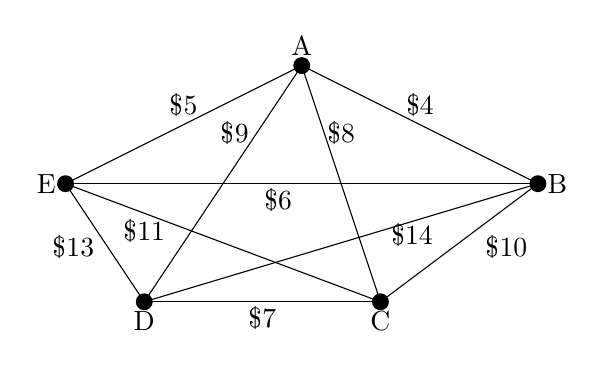
\begin{tikzpicture}
\draw[fill] (0,0) circle[radius=.1] node[below]{D};
\draw[fill] (3,0) circle[radius=.1] node[below]{C};
\draw[fill] (-1,1.5) circle[radius=.1] node[left]{E};
\draw[fill] (2,3) circle[radius=.1] node[above]{A};
\draw[fill] (5,1.5) circle[radius=.1] node[right]{B};
\draw(0,0)--(3,0);
\draw(0,0)--(2,3);
\draw(0,0)--(-1,1.5);
\draw(0,0)--(5,1.5);
\draw(3,0)--(-1,1.5);
\draw(3,0)--(2,3);
\draw(3,0)--(5,1.5);
\draw(-1,1.5)--(2,3);
\draw(-1,1.5)--(5,1.5);
\draw(2,3)--(5,1.5);
\node at (1.5, -0.2){\$7};
\node at (-0.9, 0.7){\$13};
\node at (4.6,0.7){\$10};
\node at (3.5, 2.5){\$4};
\node at (0.5,2.5){\$5};
\node at (1.7,1.3){\$6};
\node at (1.15,2.15){\$9};
\node at (2.5,2.15){\$8};
\node at (0,0.9){\$11};
\node at (3.4,0.85){\$14};
\end{tikzpicture}\par\captionof{figure}{Pohon merentang 4 simpul yang digambar sebagai titik penuh di sudut-sudut wilayah kecil dan dihubungkan oleh tiga...}\label{fig:graphtheory-dor1-tikz23}% fig-num-auto

\end{center}

Dalam kasus ini, kita tidak perlu menemukan sirkuit, bahkan tidak perlu menemukan lintasan tertentu; kita hanya perlu memastikan bahwa panggilan dapat dilakukan dari sembarang kantor ke setiap kantor lain.  Dengan kata lain, kita harus memastikan bahwa terdapat lintasan dari sembarang simpul ke setiap simpul lain.

\begin{definition}{Pohon Merentang}
Pohon merentang adalah graf terhubung yang menggunakan semua simpul dan tidak memiliki sirkuit.  
Dengan kata lain, terdapat lintasan dari sembarang simpul ke setiap simpul lain, tetapi tidak terdapat sirkuit.   
\end{definition}

Beberapa contoh pohon merentang diperlihatkan di bawah ini.  Perhatikan bahwa tidak terdapat sirkuit pada pohon-pohon tersebut, dan simpul boleh memiliki derajat lebih besar dari dua.\\

\begin{center}
\begin{minipage}{0.19\textwidth}
\centering
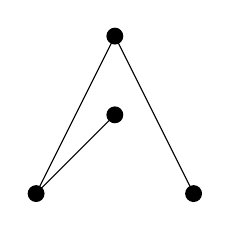
\begin{tikzpicture}
\draw[fill] (0,0) circle[radius=.1];
\draw[fill] (1,1) circle[radius=.1];
\draw[fill] (1,2) circle[radius=.1];
\draw[fill] (2,0) circle[radius=.1];
\draw(0,0)--(1,2);
\draw(0,0)--(1,1);
\draw(1,2)--(2,0);
\end{tikzpicture}

\end{minipage}
%
\begin{minipage}{0.19\textwidth}
\centering
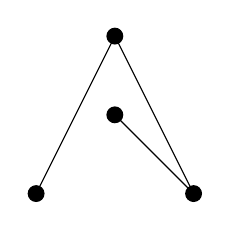
\begin{tikzpicture}
\draw[fill] (0,0) circle[radius=.1];
\draw[fill] (1,1) circle[radius=.1];
\draw[fill] (1,2) circle[radius=.1];
\draw[fill] (2,0) circle[radius=.1];
\draw(0,0)--(1,2);
\draw(2,0)--(1,1);
\draw(1,2)--(2,0);
\end{tikzpicture}

\end{minipage}
%
\begin{minipage}{0.19\textwidth}
\centering
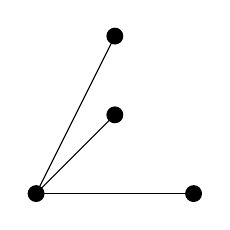
\begin{tikzpicture}
\draw[fill] (0,0) circle[radius=.1];
\draw[fill] (1,1) circle[radius=.1];
\draw[fill] (1,2) circle[radius=.1];
\draw[fill] (2,0) circle[radius=.1];
\draw(0,0)--(1,2);
\draw(0,0)--(1,1);
\draw(0,0)--(2,0);
\end{tikzpicture}
\end{minipage}
%
\begin{minipage}{0.19\textwidth}
\centering
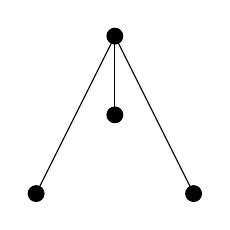
\begin{tikzpicture}
\draw[fill] (0,0) circle[radius=.1];
\draw[fill] (1,1) circle[radius=.1];
\draw[fill] (1,2) circle[radius=.1];
\draw[fill] (2,0) circle[radius=.1];
\draw(0,0)--(1,2);
\draw(1,2)--(1,1);
\draw(1,2)--(2,0);
\end{tikzpicture}
\end{minipage}
%
\begin{minipage}{0.19\textwidth}
\centering
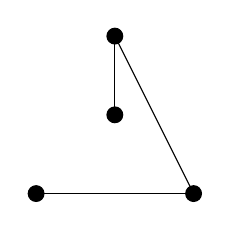
\begin{tikzpicture}
\draw[fill] (0,0) circle[radius=.1];
\draw[fill] (1,1) circle[radius=.1];
\draw[fill] (1,2) circle[radius=.1];
\draw[fill] (2,0) circle[radius=.1];
\draw(1,1)--(1,2);
\draw(1,2)--(2,0);
\draw(0,0)--(2,0);
\end{tikzpicture}
\end{minipage}
\par\smallskip
\captionof{figure}{Lima contoh pohon merentang pada graf dengan empat simpul.}
\label{fig:graphtheory-dor1-tikz24}\label{fig:graphtheory-dor1-tikz25}% fig-num-auto
\end{center}

Biasanya kita memiliki graf awal untuk diolah, seperti dalam contoh telepon di atas.  Dalam kasus ini, kita membentuk pohon merentang dengan menemukan sebuah \textbf{subgraf}, yaitu graf baru yang dibentuk menggunakan semua simpul tetapi hanya sebagian sisi dari graf semula.  Tidak ada sisi yang dibuat di tempat yang sebelumnya tidak memiliki sisi.

\textbf{Pertanyaan: Berapa banyak sisi yang terdapat dalam pohon merentang suatu graf terhubung?}

\begin{figure}[h!]
\centering
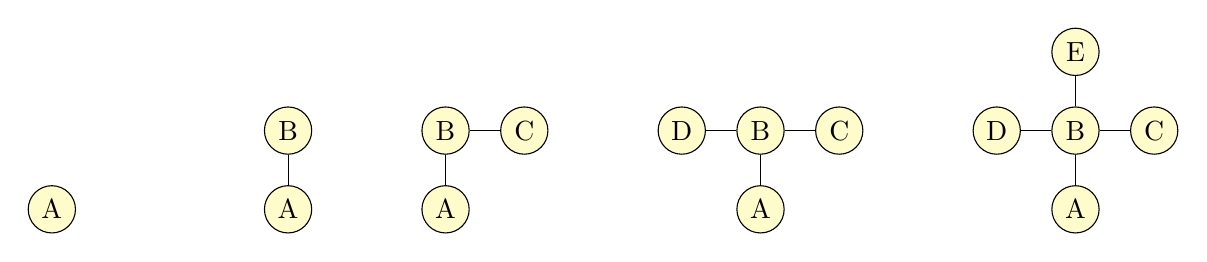
\begin{tikzpicture}[scale=1, every node/.style={circle, draw, fill=yellow!20, minimum size=6mm, inner sep=1pt}]

% n = 1
\node (A1) at (0,0) {A};

% n = 2
\node (A2) at (3,0) {A};
\node (B2) at (3,1) {B};
\draw (A2) -- (B2);

% n = 3
\node (A3) at (5,0) {A};
\node (B3) at (5,1) {B};
\node (C3) at (6,1) {C};
\draw (A3) -- (B3);
\draw (B3) -- (C3);

% n = 4
\node (A4) at (9,0) {A};
\node (B4) at (9,1) {B};
\node (C4) at (10,1) {C};
\node (D4) at (8,1) {D};
\draw (A4) -- (B4);
\draw (B4) -- (C4);
\draw (B4) -- (D4);

% n = 5
\node (A5) at (13,0) {A};
\node (B5) at (13,1) {B};
\node (C5) at (14,1) {C};
\node (D5) at (12,1) {D};
\node (E5) at (13,2) {E};
\draw (A5) -- (B5);
\draw (B5) -- (C5);
\draw (B5) -- (D5);
\draw (B5) -- (E5);

\end{tikzpicture}\\
\vspace{1cm}

\caption{Contoh pohon merentang dengan \( n = 1, 2, 3, 4, 5 \) simpul dan tepat \( n-1 \) sisi}
\end{figure}

\begin{lemma}{Banyaknya Sisi dalam Pohon Merentang}
Misalkan \( G = (V, E) \) adalah graf tak berarah terhubung dengan \( |V| = n \).  
Maka setiap pohon merentang dari \( G \) memuat tepat \( n - 1 \) sisi.
\end{lemma}

\begin{proof}[Gagasan pembuktian]
Kita membuktikannya dengan induksi pada banyaknya simpul \( n \).

\textbf{Kasus dasar (\( n = 1 \)):}  
Pohon dengan satu simpul dan tanpa sisi secara trivial memenuhi sifat \( |E| = 1 - 1 = 0 \).

\begin{center}
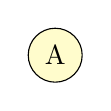
\begin{tikzpicture}
    \node[circle, draw, fill=yellow!20] (A) at (0,0) {A};
\end{tikzpicture}
\captionof{figure}{Kasus dasar: Satu simpul tanpa sisi}
\end{center}

\textbf{Langkah induksi:}  
Asumsikan bahwa setiap pohon dengan \( k \) simpul memiliki tepat \( k - 1 \) sisi.

Sekarang tinjau sebuah pohon dengan \( k + 1 \) simpul. Setiap pohon memiliki sedikitnya satu daun (simpul berderajat 1). Hapus satu daun dan satu-satunya sisi yang bersisian dengannya. Graf yang dihasilkan tetap berupa pohon (terhubung dan asiklik) dengan \( k \) simpul.

Berdasarkan hipotesis induksi, pohon yang lebih kecil ini memiliki \( k - 1 \) sisi. Dengan menambahkan kembali daun yang dihapus beserta sisinya, diperoleh total \( k \) sisi, yang sama dengan \( (k + 1) - 1 \).

\begin{center}
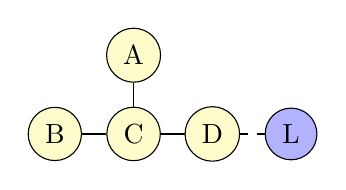
\begin{tikzpicture}[scale=1]
    \node[circle, draw, fill=yellow!20] (A) at (0,1) {A};
    \node[circle, draw, fill=yellow!20] (B) at (-1,0) {B};
    \node[circle, draw, fill=yellow!20] (C) at (0,0) {C};
    \node[circle, draw, fill=yellow!20] (D) at (1,0) {D};
    \node[circle, draw, fill=blue!30] (L) at (2,0) {L};

    \draw (A) -- (C);
    \draw (B) -- (C);
    \draw (D) -- (C);
    \draw[dashed, thick] (D) -- (L);
\end{tikzpicture}
\vspace{1cm}
\captionof{figure}{Langkah induksi: Menghapus daun \( L \) dan sisi putus-putusnya menyusutkan pohon menjadi 4 simpul dan 3 sisi}
\end{center}

Jadi, berdasarkan induksi, setiap pohon dengan \( n \) simpul memiliki tepat \( n - 1 \) sisi.
\end{proof}

Tentu saja, sembarang pohon merentang bukanlah yang benar-benar kita inginkan.  Kita menginginkan \textbf{pohon merentang biaya minimum (MCST)}.

\begin{definition}{Pohon Merentang Biaya Minimum (MCST)}
Pohon merentang biaya minimum adalah pohon merentang dengan bobot total sisi yang paling kecil.  
\end{definition}

\textbf{Penerapan Pohon Merentang Biaya Minimum (MCST):}
\begin{enumerate}
    \item \textbf{Perancangan Jaringan:} Saat memasang kabel serat optik, pipa air, atau kabel listrik untuk menghubungkan sekumpulan kota atau bangunan, kita ingin memastikan konektivitas penuh dengan biaya pemasangan terendah. MCST memberikan cara termurah untuk menghubungkan semua lokasi tanpa membuat gelang.

    \item \textbf{Infrastruktur Transportasi:} Seorang perencana transportasi mungkin perlu menghubungkan sekumpulan kota dengan jalan sambil meminimalkan biaya konstruksi total. MCST menyediakan rencana untuk menghubungkan semua kota tanpa jalan yang berlebihan.

    \item \textbf{Pengelompokan dalam Pembelajaran Mesin:} Dalam pengelompokan hierarkis, titik data dapat dipandang sebagai simpul pada graf, dengan sisi yang dibobot menurut jarak berpasangan. MCST menangkap struktur data, dan penghapusan sisi terbesar dapat mengungkap kelompok-kelompok alami.

    \item \textbf{Jaringan Komunikasi yang Andal:} Untuk konektivitas dasar dalam sistem komunikasi (misalnya jaringan komputer atau telekomunikasi), MCST memastikan semua perangkat terhubung dengan biaya total pengabelan yang minimum sehingga menyediakan jaringan dasar.

    \item \textbf{Subrutin dalam Algoritme Aproksimasi:} MCST digunakan sebagai subrutin utama dalam algoritme aproksimasi untuk masalah NP-sukar, seperti Masalah Wiraniaga Keliling (TSP). Sebagai contoh, aproksimasi-2 untuk TSP metrik diawali dengan membangun pohon merentang minimum sebagai panduan untuk menyusun tur.
\end{enumerate}

\subsection{Algoritme Kruskal untuk Pohon Merentang Biaya Minimum}
\label{subsec:gt-kruskal}
Algoritme Kruskal ternyata sangat sederhana.  Algoritme ini membangun pohon merentang satu sisi demi satu sisi dengan memilih sisi termurah berikutnya untuk ditambahkan.  Namun, sisi tersebut dilewati jika penambahannya akan membentuk siklus.

Berikut adalah deskripsi algoritmenya:
\begin{algorithm}[H]
\caption{Algoritme Kruskal (Versi Deskriptif)}
\begin{algorithmic}[1]
\State \textbf{Masukan:} Graf tak berarah terhubung \( G = (V, E) \) dengan bobot sisi \( w(e) \).
\State \textbf{Inisialisasi:} Tandai semua sisi sebagai belum digunakan. Tetapkan \( T \gets \emptyset \).
\Repeat
  \State Pilih sisi termurah pada graf yang belum digunakan.
  \If{penambahan sisi tersebut akan membentuk siklus}
    \State Lewati sisi ini.
  \Else
    \State Tambahkan sisi tersebut ke \( T \).
  \EndIf
\Until{\( T \) memuat \( |V| - 1 \) sisi (yakni, sebuah pohon merentang telah terbentuk).}
\State \textbf{Keluaran:} Himpunan \( T \), yang membentuk pohon merentang minimum dari \( G \).
\end{algorithmic}
\end{algorithm}

Dalam pseudocode, algoritme tersebut tampak sebagai berikut:
\begin{algorithm}[H]
\caption{Algoritme Kruskal}
\begin{algorithmic}[1]
\State \textbf{Masukan:} Graf tak berarah terhubung \( G = (V, E) \) dengan bobot \( w(e) \) pada setiap sisi \( e \in E \).
\State \textbf{Inisialisasi:}
  \begin{itemize}
    \item Tetapkan \( T \gets \emptyset \).
    \item Urutkan semua sisi \( E \) menurut bobot yang tidak menurun.
  \end{itemize}
\For{setiap sisi \( e \in E \) dalam urutan tersebut}
  \If{penambahan \( e \) ke \( T \) tidak membentuk siklus}
    \State Tambahkan \( e \) ke \( T \).
  \EndIf
  \If{\( T \) memuat \( |V| - 1 \) sisi}
    \State \textbf{berhenti}
  \EndIf
\EndFor
\State \textbf{Keluaran:} Himpunan \( T \), yang membentuk pohon merentang minimum.
\end{algorithmic}
\end{algorithm}
\begin{example}{} %22
Dengan menggunakan graf jalur telepon di atas, mulailah menambahkan sisi:\\
\begin{minipage}{.54\textwidth}
\begin{tabular}{lll}
AB&	\$4&	OK\\
AE	&\$5	&OK\\
BE	&\$6&	tolak -- menutup sirkuit ABEA\\
DC	&\$7&	OK\\
AC&\$8&	OK\\
\end{tabular}
\end{minipage}
%
\begin{minipage}{.45\textwidth}
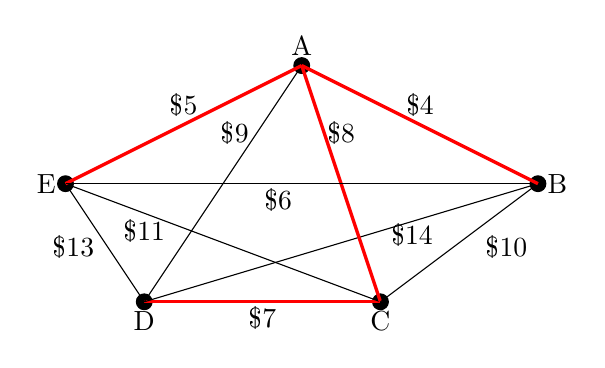
\begin{tikzpicture}
\draw[fill] (0,0) circle[radius=.1] node[below]{D};
\draw[fill] (3,0) circle[radius=.1] node[below]{C};
\draw[fill] (-1,1.5) circle[radius=.1] node[left]{E};
\draw[fill] (2,3) circle[radius=.1] node[above]{A};
\draw[fill] (5,1.5) circle[radius=.1] node[right]{B};
\draw[very thick, red](0,0)--(3,0);
\draw(0,0)--(2,3);
\draw(0,0)--(-1,1.5);
\draw(0,0)--(5,1.5);
\draw(3,0)--(-1,1.5);
\draw[very thick, red](3,0)--(2,3);
\draw(3,0)--(5,1.5);
\draw[very thick, red](-1,1.5)--(2,3);
\draw(-1,1.5)--(5,1.5);
\draw[very thick, red](2,3)--(5,1.5);
\node at (1.5, -0.2){\$7};
\node at (-0.9, 0.7){\$13};
\node at (4.6,0.7){\$10};
\node at (3.5, 2.5){\$4};
\node at (0.5,2.5){\$5};
\node at (1.7,1.3){\$6};
\node at (1.15,2.15){\$9};
\node at (2.5,2.15){\$8};
\node at (0,0.9){\$11};
\node at (3.4,0.85){\$14};
\end{tikzpicture}\par\captionof{figure}{Graf lima simpul dengan kota A, B, C, D, E sebagai titik hitam, terhubung lengkap oleh sisi berbiaya dolar...}\label{fig:graphtheory-dor1-tikz32}% fig-num-auto

\end{minipage}

Pada tahap ini kita berhenti: setiap simpul kini terhubung, sehingga kita telah membentuk pohon merentang dengan biaya \$24 ribu per tahun.
\end{example}

Algoritme Kruskal bersifat optimal sekaligus efisien; kita dijamin selalu menghasilkan MCST yang optimal.

\begin{example}{} %23
Perusahaan listrik perlu memasang jalur distribusi baru yang menghubungkan sepuluh kota di Oregon berikut ke jaringan listrik.  Bagaimana perusahaan dapat meminimalkan panjang jalur baru yang harus dipasang?
 
\begin{center}
\small
\begin{tabular}{|l|c|c|c|c|c|c|c|c|c|c|}
\hline
&&&&&&&&&&\\[7ex]
& \begin{rotate}{90}Ashland \end{rotate}& \begin{rotate}{90}Astoria\end{rotate}  & \begin{rotate}{90}Bend \end{rotate}& \begin{rotate}{90}Corvallis \end{rotate} & \begin{rotate}{90}Crater Lake \end{rotate} &  \begin{rotate}{90}Eugene  \end{rotate}&  \begin{rotate}{90}Newport \end{rotate} &  \begin{rotate}{90}Portland  \end{rotate}& \begin{rotate}{90}Salem \end{rotate} &  \begin{rotate}{90}Seaside \end{rotate}\\
\hline
Ashland & --&374&200&223&108&178&252&285&240&356\\
\hline
Astoria & 374&--&255&166&433&199&135&95&136&17\\
\hline
Bend & 200 & 255 &--&128&277&128&180 & 160&131&247\\
\hline
Corvallis&223&166&128&--&430&47&52&84&40&155\\
\hline
Crater Lake &108&433&277&430&--&453&478&344&389&423\\
\hline
Eugene &178&199&128&47&453&--&91&110&64&181\\
\hline
Newport&252&135&180&52&478&91&--&114&83&117\\
\hline
Portland &285&95&160&84&344&110&114&--&47&78\\
\hline
Salem & 240 &136&131&40&389&64&83&47&--&118\\
\hline
Seaside&356&17&247&155&423&181&117&78&118&--\\
\hline
\end{tabular}
\end{center}

Dengan algoritme Kruskal, kita menambahkan sisi mulai dari yang termurah sampai yang termahal dan menolak sisi mana pun yang menutup sirkuit.  Kita berhenti ketika graf telah terhubung.\\

\begin{minipage}{0.5\textwidth}
\small
\begin{tabular}{ll}
Seaside ke Astoria&		17 mil\\
Corvallis ke Salem	&	40 mil\\
Portland ke Salem	&	47 mil\\
Corvallis ke Eugene	&	47 mil\\
Corvallis ke Newport	&	52 mil\\
Salem ke Eugene	&	tolak -- menutup sirkuit\\
Portland ke Seaside	&	78 mil\\
\end{tabular}\\

Graf hingga tahap ini diperlihatkan di sebelah kanan.
\end{minipage}
%
\begin{minipage}{0.47\textwidth}
\scalebox{0.7}{
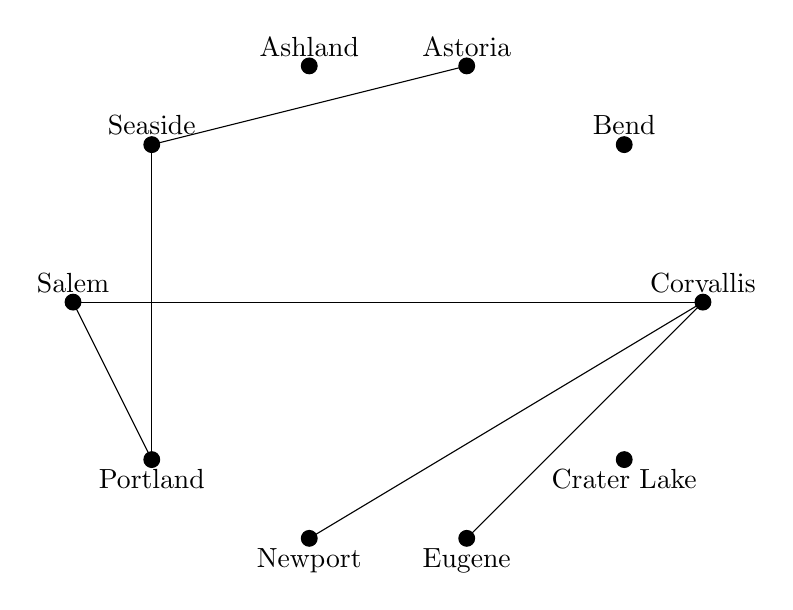
\begin{tikzpicture}
\draw[fill] (2,-2) circle[radius=.1] node[below]{Portland};
\draw[fill] (1,0) circle[radius=.1] node[above]{Salem};
\draw[fill] (9,0) circle[radius=.1] node[above]{Corvallis};
\draw[fill] (2,2) circle[radius=.1] node[above]{Seaside};
\draw[fill] (4,3) circle[radius=.1] node[above]{Ashland};
\draw[fill] (4,-3) circle[radius=.1] node[below]{Newport};
\draw[fill] (6,3) circle[radius=.1] node[above]{Astoria};
\draw[fill] (6,-3) circle[radius=.1] node[below]{Eugene};
\draw[fill] (8,2) circle[radius=.1] node[above]{Bend};
\draw[fill] (8,-2) circle[radius=.1] node[below]{Crater Lake};
\draw(1,0)--(9,0);
\draw(1,0)--(2,-2);
\draw(2,2)--(6,3);
\draw(9,0)--(4,-3);
\draw(9,0)--(6,-3);
\draw(2,2)--(2,-2);
\end{tikzpicture}
}\par\captionof{figure}{Sebuah subgraf merentang dari graf kota-kota Oregon.}\label{fig:graphtheory-dor1-tikz33}% fig-num-auto

\end{minipage}

Selanjutnya,

\begin{minipage}{0.5\textwidth}
\small
\begin{tabular}{ll}
Newport ke Salem&		tolak \\
Corvallis ke Portland&		tolak\\ 
Eugene ke Newport	&	tolak\\
Portland ke Astoria	&	tolak\\
Ashland ke Crater Lake	&	108 mil\\
Eugene ke Portland	&	tolak \\
Newport ke Portland	&	tolak\\
Newport ke Seaside	&	tolak \\
Salem ke Seaside	&	tolak\\
Bend ke Eugene	&	128 mil\\
Bend ke Salem		&	tolak \\
Astoria ke Newport 	&	tolak \\
Salem ke Astoria 	&	tolak \\
Corvallis ke Seaside	&	tolak \\
Portland ke Bend	&	tolak \\
Astoria ke Corvallis	&	tolak \\
Eugene ke Ashland	&	178 mil\\
\end{tabular}\\

Penambahan ini menghubungkan graf.  Panjang total kabel yang harus dipasang adalah 695 mil.
\end{minipage}
%
\begin{minipage}{0.47\textwidth}
\vspace{1in}
\scalebox{0.7}{
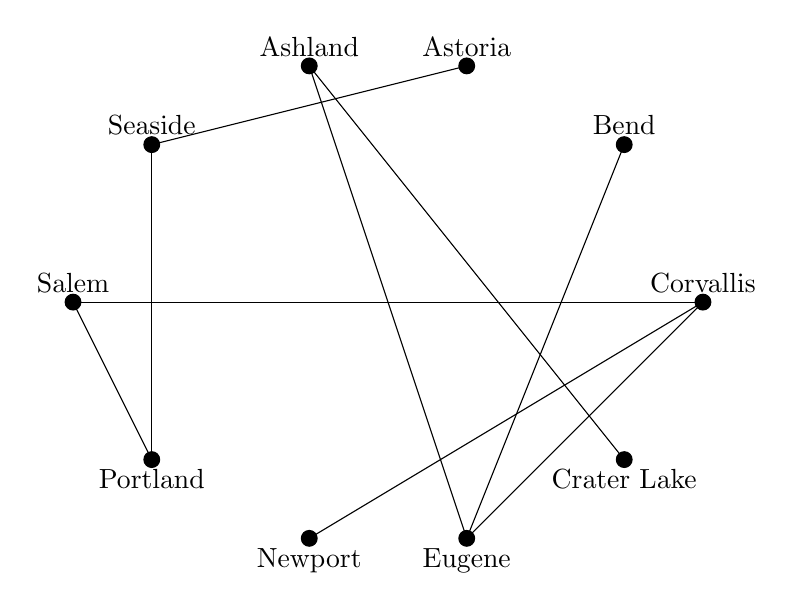
\begin{tikzpicture}
\draw[fill] (2,-2) circle[radius=.1] node[below]{Portland};
\draw[fill] (1,0) circle[radius=.1] node[above]{Salem};
\draw[fill] (9,0) circle[radius=.1] node[above]{Corvallis};
\draw[fill] (2,2) circle[radius=.1] node[above]{Seaside};
\draw[fill] (4,3) circle[radius=.1] node[above]{Ashland};
\draw[fill] (4,-3) circle[radius=.1] node[below]{Newport};
\draw[fill] (6,3) circle[radius=.1] node[above]{Astoria};
\draw[fill] (6,-3) circle[radius=.1] node[below]{Eugene};
\draw[fill] (8,2) circle[radius=.1] node[above]{Bend};
\draw[fill] (8,-2) circle[radius=.1] node[below]{Crater Lake};
\draw(1,0)--(9,0);
\draw(1,0)--(2,-2);
\draw(2,2)--(6,3);
\draw(9,0)--(4,-3);
\draw(9,0)--(6,-3);
\draw(8,-2)--(4,3);
\draw(4,3)--(6,-3);
\draw(6,-3)--(8,2);
\draw(2,2)--(2,-2);
\end{tikzpicture}
}\par\captionof{figure}{Subgraf lain dari graf kota-kota Oregon.}\label{fig:graphtheory-dor1-tikz34}% fig-num-auto

\end{minipage}

\end{example}

\begin{ex}{Pohon Merentang Biaya Minimum}
\label{ex:kruskal_exercise}
Temukan pohon merentang biaya minimum pada graf di bawah ini dengan menggunakan algoritme Kruskal.\\
\begin{center}
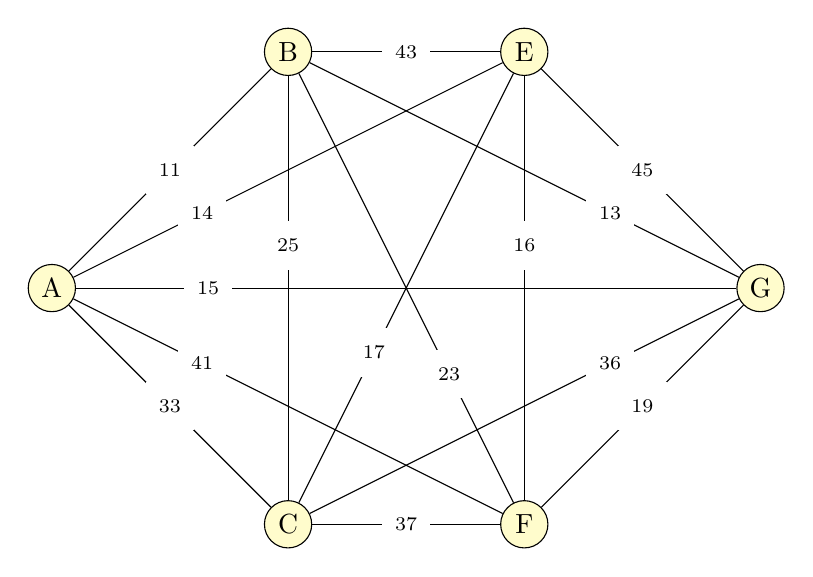
\begin{tikzpicture}[
  every node/.style={circle, draw, fill=yellow!20, minimum size=6mm, inner sep=1pt},
  edge label/.style={font=\scriptsize, rectangle, draw = white, fill=white, inner sep=2pt}
]

% Nodes
\node (A) at (0,0) {A};
\node (B) at (3,3) {B};
\node (C) at (3,-3) {C};
\node (E) at (6,3) {E};
\node (F) at (6,-3) {F};
\node (G) at (9,0) {G};

% Edges with separate edge label style
\draw (A) -- (B) node[midway, edge label] {11};
\draw (A) -- (C) node[midway, edge label] {33};
\draw (A) -- (E) node[pos=0.3, edge label] {14};
\draw (A) -- (F) node[pos=0.3, edge label] {41};
\draw (A) -- (G) node[pos=0.2, edge label] {15};

\draw (B) -- (C) node[pos=0.4, edge label] {25};
\draw (B) -- (E) node[midway, edge label] {43};
\draw (B) -- (F) node[pos=0.7, edge label] {23};
\draw (B) -- (G) node[pos=0.7, edge label] {13};

\draw (C) -- (E) node[pos=0.35, edge label] {17};
\draw (C) -- (F) node[midway, edge label] {37};
\draw (C) -- (G) node[pos=0.7, edge label] {36};

\draw (E) -- (F) node[pos=0.4, edge label] {16};
\draw (E) -- (G) node[midway, edge label] {45};
\draw (F) -- (G) node[midway, edge label] {19};

\end{tikzpicture}\par\captionof{figure}{Graf tak berarah berbobot dengan enam simpul bundar kuning A, B, C, E, F, G yang ditata membentuk segi enam.}\label{fig:graphtheory-dor1-tikz35}% fig-num-auto

\end{center}
\end{ex}

\begin{ex}{NetworkX}{}
Gunakan kode di bawah ini untuk memuat graf dari latihan sebelumnya ke dalam Python.  Kemudian selesaikan masalah ini menggunakan paket NetworkX.

\begin{lstlisting}[language=Python,
  basicstyle=\fontsize{9.5}{10.5}\selectfont\ttfamily,
  caption={Memuat graf ke dalam NetworkX},
  abovecaptionskip=6pt]
import networkx as nx

# Membuat graf tak berarah
G = nx.Graph()

# Menambahkan simpul (opsional; penambahan sisi juga menambahkan simpul)
nodes = ['A', 'B', 'C', 'E', 'F', 'G']
G.add_nodes_from(nodes)

# Menambahkan sisi berbobot
edges = [
    ('A', 'B', 11),
    ('A', 'C', 33),
    ('A', 'E', 14),
    ('A', 'F', 41),
    ('A', 'G', 15),
    ('B', 'C', 25),
    ('B', 'E', 43),
    ('B', 'F', 23),
    ('B', 'G', 13),
    ('C', 'E', 17),
    ('C', 'F', 37),
    ('C', 'G', 36),
    ('E', 'F', 16),
    ('E', 'G', 45),
    ('F', 'G', 19)
]

G.add_weighted_edges_from(edges)

# Opsional: visualisasikan graf
# nx.draw(G, with_labels=True)
# atau gunakan spring_layout atau posisi manual agar tampilan lebih jelas
\end{lstlisting}

\end{ex}

\section{Jawaban Latihan}
\begin{enumerate}[label={}, leftmargin=3.5em, labelwidth=3em, align=left]
\item[Latihan~\ref{ex:5cities}] \begin{enumerate}
\item 5 simpul, 10 sisi
\item Ya, graf tersebut terhubung.
\item Simpul tersebut berderajat 4.
\item Sebuah lintasan
\item Sebuah sirkuit\\
\end{enumerate}

\item[Latihan~\ref{ex:shortest-path}] Lintasan terpendeknya adalah ABDEG, dengan panjang 13.\\

\item[Latihan~\ref{ex:kruskal_exercise}] \hspace{.2in}\\
\begin{minipage}{0.42\linewidth}
AB: Tambahkan, biaya 11\\
BG: Tambahkan, biaya 13\\
AE: Tambahkan, biaya 14\\
AG: Lewati, akan membentuk sirkuit ABGA\\
EF: Tambahkan, biaya 16\\
EC: Tambahkan, biaya 17\\

\noindent Dengan demikian, pohon merentang telah lengkap.\\
\end{minipage}
%
\begin{minipage}{0.55\linewidth}
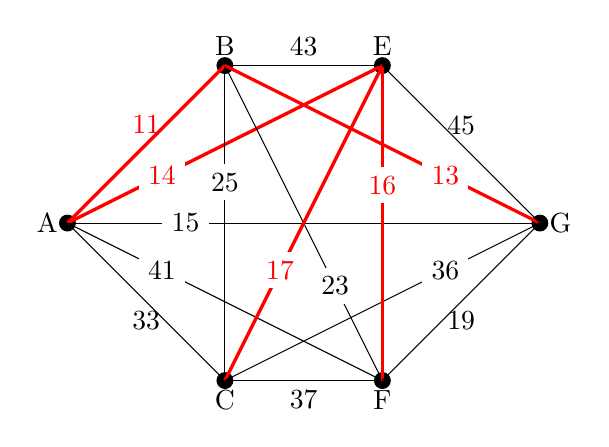
\begin{tikzpicture}
\draw[fill] (0,0) circle[radius=.1] node[left]{A};
\draw[fill] (2,2) circle[radius=.1] node[above]{B};
\draw[fill] (2,-2) circle[radius=.1] node[below]{C};
\draw[fill] (4,2) circle[radius=.1] node[above]{E};
\draw[fill] (4,-2) circle[radius=.1] node[below]{F};
\draw[fill] (6,0) circle[radius=.1] node[right]{G};
\draw[very thick, red](0,0) to node[above]{11} (2,2);
\draw(0,0) to node[below]{33}(2,-2);
\draw[very thick, red](0,0) to node[pos=0.3, fill=white]{14}(4,2);
\draw(0,0) to node[pos=0.3, fill=white]{41}(4,-2);
\draw(0,0) to node[near start, fill=white]{15}(6,0);
\draw(2,2) to node[pos=0.37, fill=white]{25}(2,-2);
\draw(2,2) to node[above]{43}(4,2);
\draw(2,2) to node[pos=0.7, fill=white]{23}(4,-2);
\draw[very thick, red](2,2) to node[pos=0.7, fill=white]{13}(6,0);
\draw[very thick, red](2,-2) to node[pos=0.35, fill=white]{17} (4,2);
\draw(2,-2) to node[below]{37}(4,-2);
\draw(2,-2) to node[pos=0.7, fill=white]{36}(6,0);
\draw[very thick, red](4,2) to node[pos=0.38, fill=white]{16}(4,-2);
\draw(4,2) to node[above]{45}(6,0);
\draw(4,-2) to node[below]{19}(6,0);
\end{tikzpicture}

\end{minipage}
\end{enumerate}

\subsection{Algoritme Prim untuk Pohon Merentang Biaya Minimum}

\begin{algorithm}[H]
\caption{Algoritme Prim (Versi Deskriptif)}
\begin{algorithmic}[1]
\State \textbf{Masukan:} Graf tak berarah terhubung \( G = (V, E) \) dengan bobot sisi \( w(e) \).
\State \textbf{Inisialisasi:} Mulai dari sembarang simpul \( v \in V \). Tetapkan \( T \gets \{v\} \) dan \( E_T \gets \emptyset \).
\Repeat
  \State Temukan sisi termurah dengan satu titik ujung di \( T \) dan titik ujung lainnya tidak di \( T \).
  \State Tambahkan sisi tersebut ke \( E_T \) dan titik ujung lainnya ke \( T \).
\Until{\( T \) mencakup semua simpul.}
\State \textbf{Keluaran:} Himpunan \( E_T \), yang membentuk pohon merentang minimum dari \( G \).
\end{algorithmic}
\end{algorithm}

Dalam pseudocode, algoritme tersebut tampak sebagai berikut:

\begin{algorithm}[H]
\caption{Algoritme Prim}
\begin{algorithmic}[1]
\State \textbf{Masukan:} Graf tak berarah terhubung \( G = (V, E) \) dengan bobot \( w(e) \) pada setiap sisi.
\State \textbf{Inisialisasi:}
  \begin{itemize}
    \item Pilih sembarang simpul awal \( v_0 \).
    \item Tetapkan \( T \gets \{v_0\} \), \( E_T \gets \emptyset \).
  \end{itemize}
\While{\( |T| < |V| \)}
  \State Di antara semua sisi \( (u, v) \in E \) dengan \( u \in T \) dan \( v \notin T \), temukan sisi dengan bobot minimum.
  \State Tambahkan \( v \) ke \( T \), dan \( (u,v) \) ke \( E_T \).
\EndWhile
\State \textbf{Keluaran:} Himpunan \( E_T \), yang membentuk pohon merentang minimum.
\end{algorithmic}
\end{algorithm}

\begin{example}{} %24
Dengan menggunakan graf jalur telepon di atas, mulailah dari simpul A dan tumbuhkan pohonnya:\\
\begin{minipage}{.54\textwidth}
\begin{tabular}{lll}
Mulai dari A&&\\
AB&	\$4&	tambahkan AB\\
AE	&\$5	&tambahkan AE\\
BE	&\$6&	tolak -- E sudah ditambahkan\\
DC	&\$7&	tambahkan DC\\
AC&\$8&	tambahkan AC\\
\end{tabular}
\end{minipage}
%
\begin{minipage}{.45\textwidth}
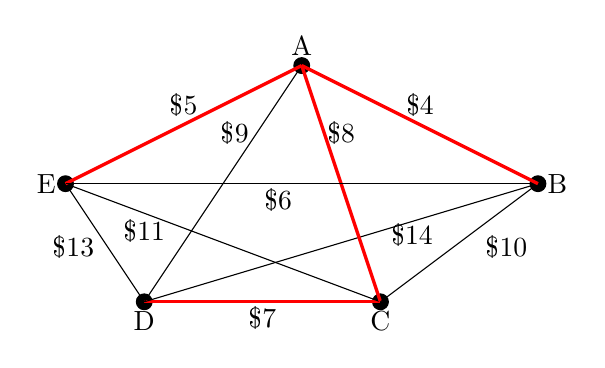
\begin{tikzpicture}
\draw[fill] (0,0) circle[radius=.1] node[below]{D};
\draw[fill] (3,0) circle[radius=.1] node[below]{C};
\draw[fill] (-1,1.5) circle[radius=.1] node[left]{E};
\draw[fill] (2,3) circle[radius=.1] node[above]{A};
\draw[fill] (5,1.5) circle[radius=.1] node[right]{B};
\draw[very thick, red](0,0)--(3,0);
\draw(0,0)--(2,3);
\draw(0,0)--(-1,1.5);
\draw(0,0)--(5,1.5);
\draw(3,0)--(-1,1.5);
\draw[very thick, red](3,0)--(2,3);
\draw(3,0)--(5,1.5);
\draw[very thick, red](-1,1.5)--(2,3);
\draw(-1,1.5)--(5,1.5);
\draw[very thick, red](2,3)--(5,1.5);
\node at (1.5, -0.2){\$7};
\node at (-0.9, 0.7){\$13};
\node at (4.6,0.7){\$10};
\node at (3.5, 2.5){\$4};
\node at (0.5,2.5){\$5};
\node at (1.7,1.3){\$6};
\node at (1.15,2.15){\$9};
\node at (2.5,2.15){\$8};
\node at (0,0.9){\$11};
\node at (3.4,0.85){\$14};
\end{tikzpicture}
\end{minipage}

Pohon merentang biaya minimum yang sama dihasilkan, dan kita berhenti setelah semua simpul ditambahkan ke pohon.
\end{example}

Seperti algoritme Kruskal, algoritme Prim dijamin menemukan pohon merentang minimum yang optimal. Namun, algoritme Prim menumbuhkan pohon dari satu akar dan menambahkan sisi penghubung termurah pada setiap langkah. Hal ini membuatnya sangat efisien jika diimplementasikan dengan antrean prioritas (misalnya menggunakan tumpukan Fibonacci untuk mencapai waktu yang hampir linear pada graf jarang).

\begin{ex}{Algoritme Prim}{}\label{ex:prim_exercise}
Gunakan algoritme Prim untuk menemukan pohon merentang biaya minimum pada graf yang sama seperti dalam Latihan~\ref{ex:kruskal_exercise}, dengan memulai dari simpul A. Perlihatkan langkah-langkah ketika Anda menambahkan sisi dan simpul ke pohon yang sedang tumbuh.
\end{ex}

\begin{figure}

\centering

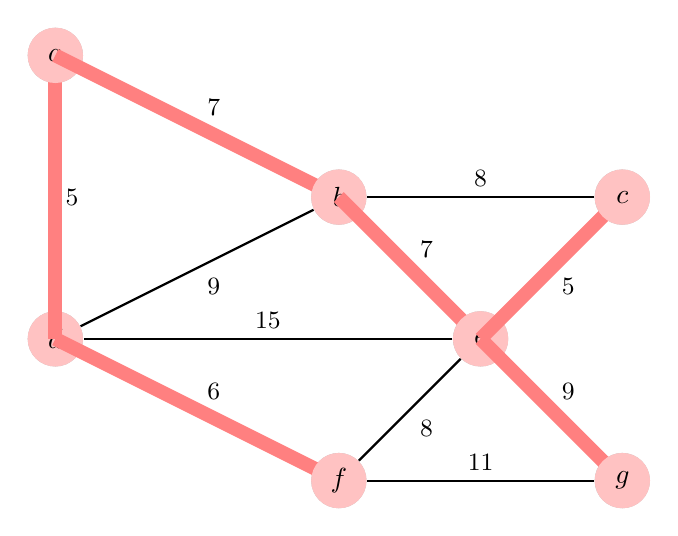
\begin{tikzpicture}[scale=1.8, auto,swap]

  % Draw a 7,11 network
  
  % First we draw the vertices
  
  \foreach \pos/\name in {{(0,2)/a}, {(2,1)/b}, {(4,1)/c},
                          {(0,0)/d}, {(3,0)/e}, {(2,-1)/f}, {(4,-1)/g}}
    \node[circle,fill=black!25,minimum size=20pt,inner sep=0pt] (\name) at \pos {$\name$};

  % Connect vertices with edges and draw weights  
  \foreach \source/ \dest / \weight in {b/a/7, c/b/8, d/a/5, d/b/9,
                                       e/b/7, e/c/5, e/d/15,
                                       f/d/6, f/e/8,
                                       g/e/9, g/f/11}
    \path[draw,thick,-] (\source) -- node[font=\small] {$\weight$} (\dest);

% solution edges

  % Vertex d
  \node[circle,fill=red!24,minimum size=20pt,inner sep=0pt] at (d) {$d$};
  
  \path[draw,line width=5pt,-,red!50] (d.center) -- (a.center);
  \path[draw,line width=5pt,-,red!50] (d.center) -- (f.center);
  
  % Vertex a 
  \node[circle,fill=red!24,minimum size=20pt,inner sep=0pt] at (a) {$a$};
  
  \path[draw,line width=5pt,-,red!50] (a.center) -- (b.center);

  % Vertex f
  \node[circle,fill=red!24,minimum size=20pt,inner sep=0pt] at (f) {$f$};

  % Vertex b
  \node[circle,fill=red!24,minimum size=20pt,inner sep=0pt] at (b) {$b$};
  
  \path[draw,line width=5pt,-,red!50] (b.center) -- (e.center);

  % Vertex e
  \node[circle,fill=red!24,minimum size=20pt,inner sep=0pt] at (e) {$e$};

  \path[draw,line width=5pt,-,red!50] (e.center) -- (c.center);
  \path[draw,line width=5pt,-,red!50] (e.center) -- (g.center);

  % Vertex c
  \node[circle,fill=red!24,minimum size=20pt,inner sep=0pt] at (c) {$c$};
  
  % Vertex g
  \node[circle,fill=red!24,minimum size=20pt,inner sep=0pt] at (g) {$g$};

\end{tikzpicture}

\caption{Algoritme Prim}

\end{figure}

\section{Latihan}

Latihan dalam bab ini disusun dalam tiga kelompok yang saling bertahap.  Butir \textbf{Keterampilan} melatih mekanisme: menerjemahkan peta dan tabel menjadi graf, menghitung derajat, serta menjalankan algoritme Dijkstra dan Kruskal dengan tangan.  Butir \textbf{Konsep} meminta Anda menjelaskan alasan algoritme bekerja dan batas-batasnya.  \textbf{Eksplorasi} merupakan kegiatan terbuka yang lebih panjang dan cocok untuk kerja kelompok.  Di dalam setiap kelompok, butir mengikuti urutan kemunculan materi dalam bab.

\begin{ex}{Masalah Lintasan Terpendek}{} %2
\label{ex:shortest-path}
Temukan lintasan terpendek antara simpul A dan G pada graf di bawah ini.\\

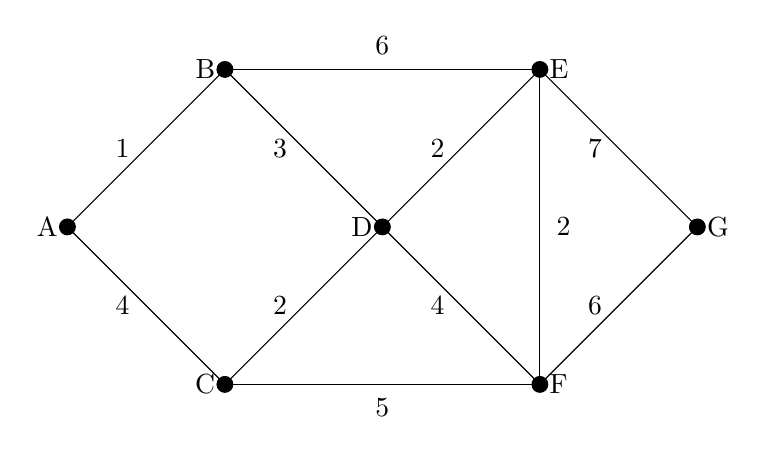
\begin{tikzpicture}
\draw[fill] (0,0) circle[radius=.1] node[left]{A};
\draw[fill] (2,2) circle[radius=.1] node[left]{B};
\draw[fill] (2,-2) circle[radius=.1] node[left]{C};
\draw[fill] (4,0) circle[radius=.1] node[left]{D};
\draw[fill] (6,2) circle[radius=.1] node[right]{E};
\draw[fill] (6,-2) circle[radius=.1] node[right]{F};
\draw[fill] (8,0) circle[radius=.1] node[right]{G};
\draw(0,0)--(2,2);
\node at (0.7,1){1};
\draw(0,0)--(2,-2);
\node at (0.7,-1){4};
\draw(2,2)--(4,0);
\node at (2.7,1){3};
\draw(2,-2)--(4,0);
\node at (2.7,-1){2};
\draw(4,0)--(6,2);
\node at (4.7,1){2};
\draw(4,0)--(6,-2);
\node at (4.7,-1){4};
\draw(6,2)--(8,0);
\node at (6.7,1){7};
\draw(6,-2)--(8,0);
\node at (6.7,-1){6};
\draw(2,2)--(6,2);
\node at (4,2.3){6};
\draw(2,-2)--(6,-2);
\node at (4,-2.3){5};
\draw(6,2)--(6,-2);
\node at (6.3,0){2};
\end{tikzpicture}\par\captionof{figure}{Gambar berbingkai untuk algoritme Prim: graf 7 simpul dengan simpul a, b, c, d, e, f, g berupa lingkaran merah.}\label{fig:graphtheory-dor1-tikz39}% fig-num-auto

\end{ex}

\textbf{Keterampilan}
\begin{enumerate}
\item	Untuk mengantarkan surat di suatu lingkungan, petugas pos perlu berjalan menyusuri setiap jalan yang memiliki rumah (titik-titik).  Buatlah graf dengan sisi yang memperlihatkan tempat petugas harus berjalan untuk mengantarkan surat.\\

\altincludegraphics{graph-theory-graphics/GraphExercise1.png}{Diagram latihan: lingkungan bergaya yang diperlihatkan sebagai enam blok persegi panjang dalam dua baris, masing-masing tiga blok. Kotak hitam pada tepi bagian dalam setiap blok menandai rumah; mahasiswa menggambar sisi di sepanjang jalan yang dilalui petugas pos untuk mencapai setiap rumah.}\\\par\captionof{figure}{Diagram latihan: lingkungan bergaya yang diperlihatkan sebagai enam blok persegi panjang dalam dua baris, masing-masing tiga blok.}\label{fig:GraphExercise1}% fig-num-auto


\item	Misalkan sebuah kota memiliki 7 jembatan seperti pada gambar di bawah ini.  Buatlah graf yang dapat digunakan untuk menentukan apakah terdapat lintasan yang menyeberangi semua jembatan tepat satu kali.\\

\altincludegraphics{graph-theory-graphics/GraphExercise2.png}{Peta latihan sebuah kota fiktif: sungai biru kehijauan membagi wilayah menjadi beberapa daratan dan tujuh batang hitam menandai jembatan. Mahasiswa mengubah peta menjadi graf untuk menguji adanya lintasan Euler yang menyeberangi setiap jembatan satu kali.}\\\par\captionof{figure}{Peta latihan sebuah kota fiktif: sungai biru kehijauan membagi wilayah menjadi beberapa daratan, dengan...}\label{fig:GraphExercise2}% fig-num-auto


\item	Tabel di bawah ini memperlihatkan perkiraan waktu berkendara (dalam menit, tanpa kemacetan) di antara lima kota di wilayah Dallas.  Buatlah graf berbobot yang merepresentasikan data ini.
\begin{center}
\begin{tabular}{|l|c|c|c|c|}
\hline
&Plano&Mesquite&Arlington&Denton\\
\hline
Fort Worth&54&52&19&42\\
\hline
Plano&&38&53&41\\
\hline
Mesquite&&&43&56\\
\hline
Arlington&&&&50\\
\hline
\end{tabular}
\par\captionof{table}{Perkiraan waktu berkendara dalam menit di antara lima kota di wilayah Dallas.}\label{tab:graphtheory-dor1-tab02}% tab-num-auto

\end{center}

\item	Tabel di bawah ini memperlihatkan harga tiket pesawat sekali jalan di antara 5 kota\footnote{Harga termurah yang ditemukan ketika data diambil pada 1 September 2009 untuk perjalanan pada 22 September 2009}.  Buatlah graf yang memperlihatkan data ini.
\begin{center}
\begin{tabular}{|l|c|c|c|c|}
\hline
&Honolulu&London&Moscow&Cairo\\
\hline
Seattle &\$159 &\$370&\$654&\$684\\
\hline
Honolulu&&\$830&\$854&\$801\\
\hline
London&&&\$245&\$323\\
\hline
Moscow&&&&\$329\\
\hline
\end{tabular}
\par\captionof{table}{Harga tiket pesawat sekali jalan di antara lima kota.}\label{tab:graphtheory-dor1-tab03}% tab-num-auto

\end{center}

\item	Temukan derajat setiap simpul pada graf di bawah ini.\\

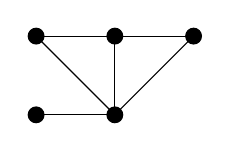
\begin{tikzpicture}
\draw[fill] (0,0) circle[radius=.1];
\draw[fill] (1,0) circle[radius=.1];
\draw[fill] (0,1) circle[radius=.1];
\draw[fill] (1,1) circle[radius=.1];
\draw[fill] (2,1) circle[radius=.1];
\draw(0,0)--(1,0);
\draw(1,0)--(1,1);
\draw(1,0)--(0,1);
\draw(1,1)--(0,1);
\draw(1,1)--(2,1);
\draw(2,1)--(1,0);
\end{tikzpicture}\par\captionof{figure}{Graf berbobot tujuh simpul untuk latihan lintasan terpendek.}\label{fig:graphtheory-dor1-tikz40}% fig-num-auto


\item	Temukan derajat setiap simpul pada graf di bawah ini.\\

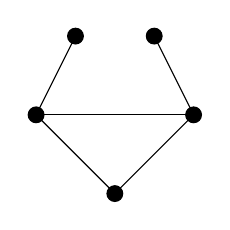
\begin{tikzpicture}
\draw[fill] (0,0) circle[radius=.1];
\draw[fill] (-1,1) circle[radius=.1];
\draw[fill] (-.5,2) circle[radius=.1];
\draw[fill] (1,1) circle[radius=.1];
\draw[fill] (.5,2) circle[radius=.1];
\draw(0,0)--(-1,1);
\draw(0,0)--(1,1);
\draw(-1,1)--(1,1);
\draw(-1,1)--(-0.5,2);
\draw(1,1)--(0.5,2);
\end{tikzpicture}\par\captionof{figure}{Tabel harga tiket pesawat yang memuat harga sekali jalan dalam dolar antara Seattle, Honolulu, London, Moskwa, dan Kairo (mis.}\label{fig:graphtheory-dor1-tikz41}% fig-num-auto


\item	Manakah di antara graf-graf ini yang terhubung?\\

\begin{tabular}{|c|c|c|}
\hline
&&\\
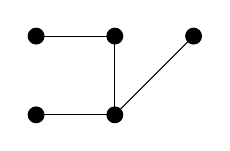
\begin{tikzpicture}
\draw[fill] (0,0) circle[radius=.1];
\draw[fill] (1,0) circle[radius=.1];
\draw[fill] (0,1) circle[radius=.1];
\draw[fill] (1,1) circle[radius=.1];
\draw[fill] (2,1) circle[radius=.1];
\draw(0,0)--(1,0);
\draw(1,0)--(1,1);
\draw(0,1)--(1,1);
\draw(1,0)--(2,1);
\end{tikzpicture}
&
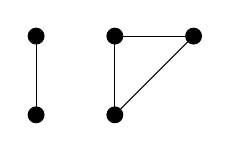
\begin{tikzpicture}
\draw[fill] (0,0) circle[radius=.1];
\draw[fill] (1,0) circle[radius=.1];
\draw[fill] (0,1) circle[radius=.1];
\draw[fill] (1,1) circle[radius=.1];
\draw[fill] (2,1) circle[radius=.1];
\draw(1,0)--(1,1);
\draw(1,0)--(2,1);
\draw(1,1)--(2,1);
\draw(0,0)--(0,1);
\end{tikzpicture}
&
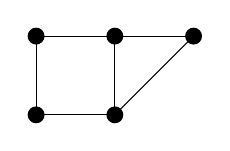
\begin{tikzpicture}
\draw[fill] (0,0) circle[radius=.1];
\draw[fill] (1,0) circle[radius=.1];
\draw[fill] (0,1) circle[radius=.1];
\draw[fill] (1,1) circle[radius=.1];
\draw[fill] (2,1) circle[radius=.1];
\draw(0,0)--(1,0);
\draw(1,0)--(1,1);
\draw(0,1)--(1,1);
\draw(1,0)--(2,1);
\draw(1,1)--(2,1);
\draw(0,0)--(0,1);
\end{tikzpicture}\\
&&\\
\hline
\end{tabular}\\\par\captionof{figure}{Tiga graf lima simpul untuk latihan keterhubungan.}\label{fig:graphtheory-dor1-connected-a}% fig-num-auto


\item Manakah di antara graf-graf ini yang terhubung?\\

\begin{tabular}{|c|c|c|}
\hline
&&\\
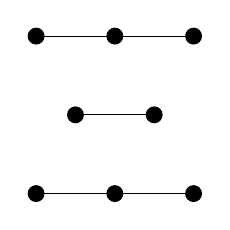
\begin{tikzpicture}
\draw[fill] (0,0) circle[radius=.1];
\draw[fill] (1,0) circle[radius=.1];
\draw[fill] (2,0) circle[radius=.1];
\draw[fill] (.5,1) circle[radius=.1];
\draw[fill] (1.5,1) circle[radius=.1];
\draw[fill] (0,2) circle[radius=.1];
\draw[fill] (1,2) circle[radius=.1];
\draw[fill] (2,2) circle[radius=.1];
\draw(0,0)--(1,0);
\draw(1,0)--(2,0);
\draw(0.5,1)--(1.5,1);
\draw(0,2)--(1,2);
\draw(1,2)--(2,2);
\end{tikzpicture}
&
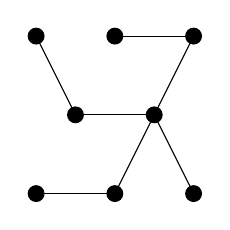
\begin{tikzpicture}
\draw[fill] (0,0) circle[radius=.1];
\draw[fill] (1,0) circle[radius=.1];
\draw[fill] (2,0) circle[radius=.1];
\draw[fill] (.5,1) circle[radius=.1];
\draw[fill] (1.5,1) circle[radius=.1];
\draw[fill] (0,2) circle[radius=.1];
\draw[fill] (1,2) circle[radius=.1];
\draw[fill] (2,2) circle[radius=.1];
\draw(0,0)--(1,0);
\draw(1,0)--(1.5,1);
\draw(0.5,1)--(1.5,1);
\draw(0,2)--(0.5,1);
\draw(1,2)--(2,2);
\draw(1.5,1)--(2,2);
\draw(1.5,1)--(2,0);
\end{tikzpicture}
&
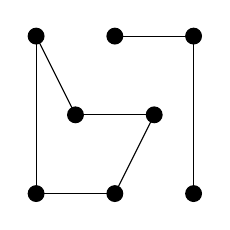
\begin{tikzpicture}
\draw[fill] (0,0) circle[radius=.1];
\draw[fill] (1,0) circle[radius=.1];
\draw[fill] (2,0) circle[radius=.1];
\draw[fill] (.5,1) circle[radius=.1];
\draw[fill] (1.5,1) circle[radius=.1];
\draw[fill] (0,2) circle[radius=.1];
\draw[fill] (1,2) circle[radius=.1];
\draw[fill] (2,2) circle[radius=.1];
\draw(0,0)--(1,0);
\draw(1,0)--(1.5,1);
\draw(0.5,1)--(1.5,1);
\draw(0,2)--(0,0);
\draw(1,2)--(2,2);
\draw(2,2)--(2,0);
\draw(0,2)--(.5,1);
\end{tikzpicture}\\
\hline
\end{tabular}\\\par\captionof{figure}{Tiga graf lain untuk latihan keterhubungan.}\label{fig:graphtheory-dor1-connected-b}% fig-num-auto


\item	\label{ex:dijkstra-eurail}Waktu perjalanan kereta untuk suatu segmen sistem Eurail diperlihatkan di bawah ini dalam jam dan menit.  Temukan lintasan dengan waktu tempuh terpendek dari Bern ke Berlin dengan menerapkan algoritme Dijkstra.\\

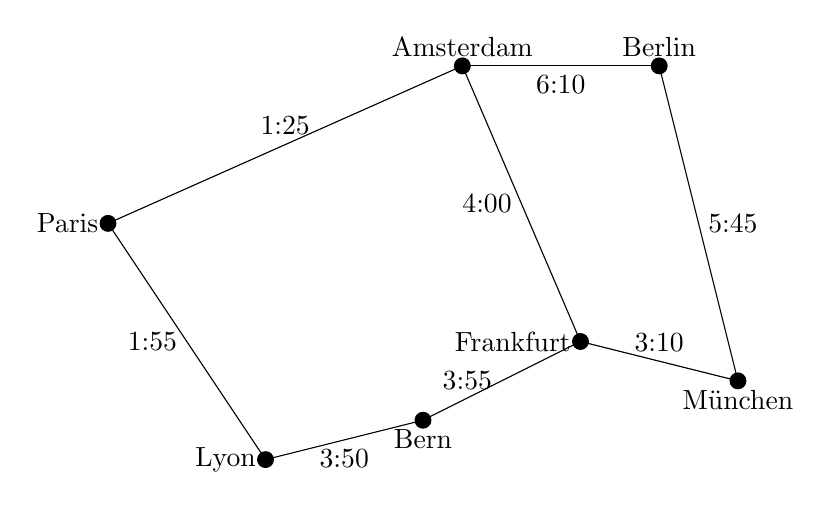
\begin{tikzpicture}
\draw[fill] (0,0) circle[radius=.1] node[left]{Paris};
\draw[fill] (2,-3) circle[radius=.1] node[left]{Lyon};
\draw[fill] (4,-2.5) circle[radius=.1] node[below]{Bern};
\draw[fill] (6,-1.5) circle[radius=.1] node[left]{Frankfurt};
\draw[fill] (8,-2) circle[radius=.1] node[below]{M\"unchen};
\draw[fill] (4.5,2) circle[radius=.1] node[above]{Amsterdam};
\draw[fill] (7,2) circle[radius=.1] node[above]{Berlin};
\draw(0,0) to node[above]{1:25} (4.5,2);
\draw(0,0) to node[left]{1:55} (2,-3);
\draw(2,-3) to node[below]{3:50} (4,-2.5);
\draw(4,-2.5) to node[left]{3:55} (6,-1.5);
\draw(6,-1.5) to node[above]{3:10} (8,-2);
\draw(6,-1.5) to node[left]{4:00} (4.5,2);
\draw(8,-2) to node[right]{5:45} (7,2);
\draw(7,2) to node[below]{6:10} (4.5,2);
\end{tikzpicture}\par\captionof{figure}{Jaringan kereta Eropa dengan waktu tempuh antarkota.}\label{fig:graphtheory-dor1-tikz48}% fig-num-auto


\item	Dengan menggunakan graf dari soal sebelumnya, temukan lintasan dengan waktu tempuh terpendek dari Paris ke M\"unchen.

\item	Temukan pohon merentang biaya minimum untuk graf yang Anda buat dalam soal \#3.\\

\item	\label{ex:mst-sonet-ring}Sebuah perusahaan ingin menghubungkan 5 bangunannya dengan kabel serat optik.  Biaya (dalam ribuan dolar) untuk memasang kabel di antara pasangan bangunan diperlihatkan di bawah ini.  Temukan pohon merentang biaya minimum yang menghubungkan bangunan-bangunan tersebut.\\

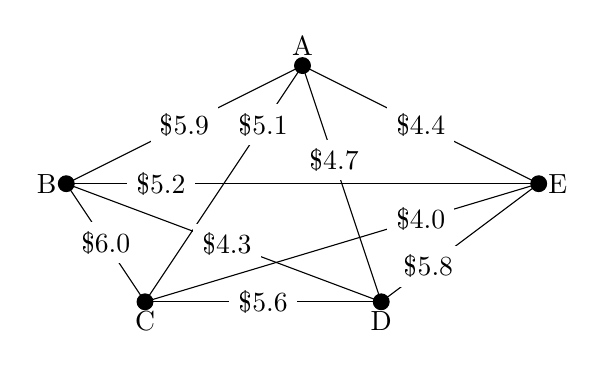
\begin{tikzpicture}
\draw(0,0)  to node[fill=white]{\$5.6}(3,0);
\draw(0,0)  to node[near end, fill=white]{\$5.1}(2,3);
\draw(0,0)  to node[fill=white]{\$6.0}(-1,1.5);
\draw(3,0)  to node[pos=0.49,fill=white]{\$4.3}(-1,1.5);
\draw(3,0)  to node[pos=0.6, fill=white]{\$4.7}(2,3);
\draw(3,0) to node[pos=0.3, fill=white]{\$5.8}(5,1.5);
\draw(-1,1.5) to node[fill=white]{\$5.9}(2,3);
\draw(-1,1.5)  to node[pos=0.2, fill=white]{\$5.2}(5,1.5);
\draw(2,3)  to node[fill=white]{\$4.4}(5,1.5);
\draw(0,0) to node[pos=0.7, fill=white]{\$4.0}(5,1.5);
\draw[fill] (0,0) circle[radius=.1] node[below]{C};
\draw[fill] (3,0) circle[radius=.1] node[below]{D};
\draw[fill] (-1,1.5) circle[radius=.1] node[left]{B};
\draw[fill] (2,3) circle[radius=.1] node[above]{A};
\draw[fill] (5,1.5) circle[radius=.1] node[right]{E};
\end{tikzpicture}\\\par\captionof{figure}{Graf berbobot pada lima simpul berlabel A, B, C, D, E dalam tata letak segi lima, terhubung lengkap oleh...}\label{fig:graphtheory-dor1-tikz49}% fig-num-auto


\item \label{ex:dijkstra-warmup-rail}Waktu perjalanan kereta penumpang dalam menit di antara lima kota di Virginia dan Washington, D.C., diperlihatkan di bawah ini.  Terapkan algoritme Dijkstra, tepat seperti pada contoh yang dikerjakan di \S\ref{sec:gt-shortest-path} dan dalam Latihan~\ref{ex:dijkstra-eurail}, untuk menemukan rute dengan waktu tempuh terpendek dari Bristol ke Washington.  Catat label jarak ketika masing-masing menjadi permanen.\\

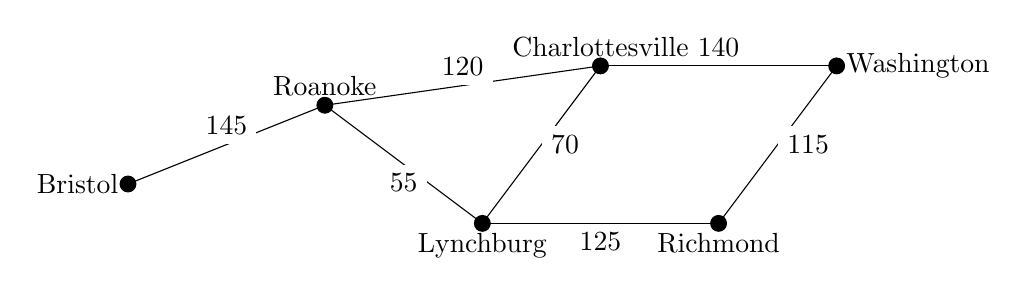
\begin{tikzpicture}
\draw[fill] (0,0) circle[radius=.1] node[left]{Bristol};
\draw[fill] (2.5,1) circle[radius=.1] node[above]{Roanoke};
\draw[fill] (4.5,-0.5) circle[radius=.1] node[below]{Lynchburg};
\draw[fill] (6,1.5) circle[radius=.1] node[above]{Charlottesville};
\draw[fill] (7.5,-0.5) circle[radius=.1] node[below]{Richmond};
\draw[fill] (9,1.5) circle[radius=.1] node[right]{Washington};
\draw(0,0) to node[above, fill=white]{145} (2.5,1);
\draw(2.5,1) to node[below, fill=white]{55} (4.5,-0.5);
\draw(2.5,1) to node[above, fill=white]{120} (6,1.5);
\draw(4.5,-0.5) to node[right, fill=white]{70} (6,1.5);
\draw(4.5,-0.5) to node[below, fill=white]{125} (7.5,-0.5);
\draw(6,1.5) to node[above, fill=white]{140} (9,1.5);
\draw(7.5,-0.5) to node[right, fill=white]{115} (9,1.5);
\end{tikzpicture}\par\captionof{figure}{Jaringan jalan kota-kota Virginia dengan jarak.}\label{fig:graphtheory-dor1-tikz50}% fig-num-auto

\exrefs{\S\ref{sec:gt-shortest-path}, Latihan~\ref{ex:dijkstra-eurail}}

\item \label{ex:kruskal-airfare}Dengan menggunakan algoritme Kruskal, temukan pohon merentang biaya minimum untuk graf harga tiket pesawat yang Anda buat dalam soal \#4.  Daftarkan sisi menurut urutan pertimbangannya oleh algoritme, dan catat setiap sisi yang ditolak karena akan menutup sirkuit.  Untuk tujuan apa sebuah aliansi maskapai menggunakan pohon semacam itu?
\exrefs{\S\ref{subsec:gt-kruskal}}
\end{enumerate}

\noindent \textbf{Konsep}

\begin{enumerate}[start=15]
\item Dapatkah sebuah graf memiliki satu simpul berderajat ganjil?  Jika tidak, adakah banyak simpul berderajat ganjil lain yang juga mustahil?  Mengapa?\\

\item \label{ex:mst-greedy}Algoritme Kruskal bersifat \emph{rakus}: pada setiap langkah, algoritme mengambil sisi termurah yang tersedia tanpa mempertimbangkan apa yang akan terjadi kemudian.  Jelaskan secara informal mengapa pandangan jangka pendek ini tidak pernah menimbulkan biaya tambahan bagi pohon merentang.  Misalkan pohon $T$ yang dihasilkan algoritme melewati suatu sisi $e$ yang dimiliki pohon merentang yang lebih murah; gunakan fakta bahwa penambahan $e$ ke $T$ menutup tepat satu sirkuit untuk berargumen bahwa pohon yang lebih murah itu dapat diperbaiki, satu sisi demi satu sisi, menjadi pohon Kruskal tanpa pernah meningkatkan biayanya.  Apakah penalaran yang sama tetap berlaku jika beberapa biaya sisi bernilai negatif?
\exrefs{\S\ref{subsec:gt-kruskal}}

\item \label{ex:dijkstra-nonneg}Algoritme Dijkstra menandai secara permanen simpul belum dikunjungi dengan jarak tercatat paling kecil dan tidak pernah mengunjunginya kembali.  Jelaskan mengapa langkah ini dapat dibenarkan ketika semua bobot sisi tidak negatif.  Kemudian buatlah graf dengan tiga simpul yang salah satu sisinya berbobot negatif dan menyebabkan algoritme menghasilkan jawaban yang salah.
\exrefs{\S\ref{sec:gt-shortest-path}}

\end{enumerate}

\noindent \textbf{Eksplorasi}

\begin{enumerate}[start=18]
\item Jejaring sosial seperti Facebook dan LinkedIn dapat direpresentasikan menggunakan graf, dengan simpul yang merepresentasikan orang dan sisi yang digambar di antara dua simpul ketika kedua orang tersebut “berteman”.   Tabel di bawah ini memperlihatkan tabel pertemanan; X menunjukkan bahwa dua orang berteman.
\begin{center}
\begin{tabular}{|c|c|c|c|c|c|c|c|c|c|}
\hline
&A&B&C&D&E&F&G&H&I\\
\hline
A & \cellcolor{yellow}&X&X&&&X&X&&\\
\hline
B& \cellcolor{yellow}& \cellcolor{yellow}&X&&X&&&&\\
\hline
C& \cellcolor{yellow}& \cellcolor{yellow}& \cellcolor{yellow}&&X&&&&\\
\hline
D& \cellcolor{yellow}& \cellcolor{yellow}& \cellcolor{yellow}& \cellcolor{yellow}&X&&&&X\\
\hline
E& \cellcolor{yellow}& \cellcolor{yellow}& \cellcolor{yellow}& \cellcolor{yellow}& \cellcolor{yellow}&&X&&X\\
\hline
F& \cellcolor{yellow}& \cellcolor{yellow}& \cellcolor{yellow}& \cellcolor{yellow}& \cellcolor{yellow}& \cellcolor{yellow}&&X&X\\
\hline
G& \cellcolor{yellow}& \cellcolor{yellow}& \cellcolor{yellow}& \cellcolor{yellow}& \cellcolor{yellow}& \cellcolor{yellow}& \cellcolor{yellow}&X&\\
\hline
H& \cellcolor{yellow}& \cellcolor{yellow}& \cellcolor{yellow}& \cellcolor{yellow}& \cellcolor{yellow}& \cellcolor{yellow}& \cellcolor{yellow}& \cellcolor{yellow}&X\\
\hline
\end{tabular}
\par\captionof{table}{Tabel pertemanan: X menandai pasangan orang yang berteman.}\label{tab:graphtheory-dor1-tab04}% tab-num-auto

\end{center}
\begin{enumerate}
\item	Buatlah graf dari tabel pertemanan ini
\item	Temukan lintasan terpendek dari A ke D.  Panjang lintasan ini sering disebut “derajat keterpisahan” kedua orang tersebut.
\item	Pengembangan:  Bagilah kelas menjadi beberapa kelompok.  Setiap kelompok memilih 10 film atau lebih dan mencari pemeran utamanya (www.imdb.com merupakan sumber yang baik).  Buatlah graf dengan setiap aktor sebagai simpul dan sisi yang menghubungkan dua aktor dalam film yang sama (catat nama film pada sisi).  Temukan lintasan yang menarik di antara para aktor, lalu berikan kuis kepada kelompok lain untuk melihat apakah mereka dapat menebak keterhubungannya.\\
\end{enumerate}

\item	Pemeriksa ejaan dalam program pengolah kata memberikan saran ketika menemukan kata yang tidak ada dalam kamus.  Untuk menentukan kata yang akan disarankan, program mencoba menemukan kata yang serupa.  Salah satu ukuran keserupaan kata adalah jarak Levenshtein, yang mengukur banyaknya penggantian, penambahan, atau penghapusan yang diperlukan untuk mengubah satu kata menjadi kata lain.   Sebagai contoh, kata spit dan spot berjarak 1; mengubah spit menjadi spot memerlukan satu penggantian (i dengan o).   Demikian pula, spit berjarak 1 dari pit karena perubahan tersebut memerlukan satu penghapusan (s).  Kata spite juga berjarak 1 dari spit karena memerlukan satu penambahan (e).  Kata soot berjarak 2 dari spit karena diperlukan dua penggantian.
\begin{enumerate}
\item	Buatlah graf dengan kata sebagai simpul dan sisi yang menghubungkan kata-kata dengan jarak Levenshtein 1.  Gunakan kata salah eja “moke” sebagai pusat, lalu cobalah menemukan sedikitnya 10 kata dalam kamus yang terhubung.  Bagaimana pemeriksa ejaan dapat menggunakan graf ini?   
\item	Perbaiki metode di atas dengan memberikan bobot pada setiap sisi berdasarkan kemungkinan terjadinya penggantian, penambahan, atau penghapusan.  Anda dapat menentukan bobot berdasarkan pendekatan apa pun yang wajar: kedekatan tombol pada papan ketik, kesalahan bahasa yang umum, dan sebagainya.  Gunakan algoritme Dijkstra untuk menemukan panjang lintasan terpendek dari setiap kata ke “moke”.  Bagaimana pemeriksa ejaan dapat menggunakan nilai-nilai ini?   \\
\end{enumerate}

\end{enumerate}

\subsubsection*{Solusi Terpilih}

\begin{solution}(Latihan~\ref{ex:dijkstra-eurail})
Jalankan algoritme Dijkstra dari Bern.  Simpul-simpul memperoleh label permanen dengan urutan: Bern (0:00), Lyon (3:50), Frankfurt (3:55), Paris (5:45, melalui Lyon), M\"unchen (7:05, melalui Frankfurt), Amsterdam (7:10, melalui Paris), Berlin (12:50, melalui M\"unchen).  Rute terpendeknya adalah
\[
\text{Bern} \to \text{Frankfurt} \to \text{M\"unchen} \to \text{Berlin},
\qquad 3{:}55 + 3{:}10 + 5{:}45 = 12{:}50.
\]
Sebagai perbandingan, Bern--Frankfurt--Amsterdam--Berlin memerlukan waktu 14:05 dan Bern--Lyon--Paris--Amsterdam--Berlin memerlukan waktu 13:20.
\end{solution}

\begin{solution}(Latihan~\ref{ex:mst-sonet-ring})
Dengan algoritme Kruskal, empat sisi termurah diterima satu demi satu tanpa penolakan: CE (4.0), BD (4.3), AE (4.4), AD (4.7).  Keempat sisi ini menghubungkan kelima bangunan, sehingga algoritme berhenti.  Pohon merentang biaya minimumnya adalah $\{CE, BD, AE, AD\}$ dengan biaya total $4.0 + 4.3 + 4.4 + 4.7 = 17.4$, yakni \$17{,}400.  (Pohon merentang merupakan cara termurah untuk menghubungkan bangunan-bangunan tersebut, tetapi tidak menyediakan lintasan cadangan jika sebuah kabel terputus.)
\end{solution}

\begin{solution}(Latihan~\ref{ex:dijkstra-warmup-rail})
Ketika algoritme Dijkstra dijalankan dari Washington, label menjadi permanen dengan urutan: Washington (0), Richmond (115), Charlottesville (140), Lynchburg (210, melalui Charlottesville), Roanoke (260, melalui Charlottesville), Bristol (405).  Rute terpendeknya adalah
\[
\text{Bristol} \to \text{Roanoke} \to \text{Charlottesville} \to \text{Washington},
\qquad 145 + 120 + 140 = 405 \text{ minutes},
\]
yaitu 6 jam 45 menit.  Sebagai perbandingan, rute melalui Lynchburg memerlukan $145 + 55 + 70 + 140 = 410$ menit dan rute melalui Richmond memerlukan $145 + 55 + 125 + 115 = 440$ menit.
\end{solution}

\begin{solution}(Latihan~\ref{ex:kruskal-airfare})
Setelah harga tiket diurutkan dari yang termurah sampai yang termahal, algoritme Kruskal menerima Seattle--Honolulu (\$159), London--Moskwa (\$245), dan London--Kairo (\$323); kemudian algoritme menolak Moskwa--Kairo (\$329) karena sisi tersebut akan menutup sirkuit London--Moskwa--Kairo, dan terakhir menerima Seattle--London (\$370), yang menghubungkan kelima kota.  Pohon merentang biaya minimum memiliki biaya total $159 + 245 + 323 + 370 = \$1097$.  Pohon semacam itu memberikan himpunan rute termurah yang tetap menghubungkan setiap kota, walaupun setiap perjalanan di antara kota-kota pada cabang yang berbeda harus terhubung melalui persinggahan perantara.
\end{solution}

\begin{solution}(Latihan~\ref{ex:mst-greedy})
Misalkan suatu pohon merentang $T^*$ menggunakan sisi $e$ yang dilewati oleh pohon Kruskal $T$.  Algoritme Kruskal menolak $e$ hanya karena, ketika $e$ diperiksa, $e$ menutup sirkuit bersama sisi-sisi yang telah diterima; karena sisi diperiksa dari yang termurah sampai yang termahal, biaya setiap sisi pada sirkuit itu tidak lebih besar daripada $e$.  Sirkuit tersebut pasti memuat suatu sisi $f \notin T^*$ (sebuah pohon tidak dapat memuat seluruh sirkuit).  Mengganti $e$ dengan $f$ dalam $T^*$ menghasilkan pohon merentang lain yang tidak lebih mahal dan bersepakat dengan $T$ pada satu sisi tambahan.  Dengan mengulangi pertukaran ini, $T^*$ berubah menjadi $T$ tanpa pernah meningkatkan biaya, sehingga $T$ setidaknya semurah setiap pohon merentang lain.  Argumen tersebut tidak pernah menggunakan tanda biaya, hanya urutannya, sehingga tetap berlaku untuk biaya sisi negatif; perhatikan perbedaannya dengan algoritme Dijkstra, yang memang bergantung pada bobot tak negatif (Latihan~\ref{ex:dijkstra-nonneg}).
\end{solution}

\ifdefined \old

\section{Sirkuit Euler dan Masalah Tukang Pos Tiongkok}
Pada bagian pertama, kita membuat graf jembatan K\"onigsberg dan bertanya apakah setiap jembatan dapat diseberangi tepat satu kali.  Karena Euler merupakan orang pertama yang mengkaji pertanyaan ini, jenis lintasan tersebut dinamai menurut namanya.

\begin{definition}{Lintasan Euler}
\textbf{Lintasan Euler} adalah lintasan yang menggunakan setiap sisi dalam graf tanpa pengulangan.  Karena berupa lintasan, lintasan Euler tidak harus kembali ke simpul awal.
\end{definition}

\begin{example}{}%5
Pada graf yang diperlihatkan di bawah ini, terdapat beberapa lintasan Euler.  Salah satunya adalah CABDCB.  Lintasan tersebut ditampilkan dengan panah di sebelah kanan dan urutan sisi diberi nomor.\\
\begin{minipage}{.5\textwidth}
\begin{center}
\scalebox{.8}{
\begin{tikzpicture}
\draw[fill] (0,0) circle[radius=.1] node [left]{B};
\draw[fill] (4,0) circle[radius=.1] node [right]{C};
\draw[fill] (2,2) circle[radius=.1] node [above]{D};
\draw[fill] (2,4) circle[radius=.1] node [above]{A};
\draw(0,0)--(4,0);
\draw(0,0)--(2,2);
\draw(0,0)--(2,4);
\draw(4,0)--(2,2);
\draw(4,0)--(2,4);
\end{tikzpicture}
}
\end{center}
\end{minipage}
%
\begin{minipage}{.5\textwidth}
\begin{center}
\scalebox{0.8}{
\begin{tikzpicture}
\draw[fill] (0,0) circle[radius=.1] node [left]{B};
\draw[fill] (4,0) circle[radius=.1] node [right]{C};
\draw[fill] (2,2) circle[radius=.1] node [above]{D};
\draw[fill] (2,4) circle[radius=.1] node [above]{A};
\draw[directed](4,0)--(0,0);
\draw[directed](0,0)--(2,2);
\draw[directed] (2,4)--(0,0);
\draw[directed](2,2)--(4,0);
\draw[directed] (4,0)--(2,4);
\node at (2,-0.3){5};
\node at (1.4,1){3};
\node at (0.7,2.2){2};
\node at (2.7,1){4};
\node at (3.3,2.2){1};
\end{tikzpicture}
}
\end{center}
\end{minipage}
\end{example}

\begin{definition}{Sirkuit Euler}
\textbf{Sirkuit Euler} adalah sirkuit yang menggunakan setiap sisi dalam graf tanpa pengulangan.  Karena berupa sirkuit, sirkuit Euler harus berawal dan berakhir pada simpul yang sama.
\end{definition}

\begin{example}{}%6
Graf di bawah ini memiliki beberapa kemungkinan sirkuit Euler.  Berikut dua di antaranya, yang berawal dan berakhir di simpul A: ADEACEFCBA dan AECABCFEDA.  Sirkuit kedua ditampilkan dengan panah.\\
\begin{minipage}{.5\textwidth}
\begin{center}
\scalebox{0.8}{
\begin{tikzpicture}
\draw[fill] (0,0) circle[radius=.1] node [below]{D};
\draw[fill] (0,2) circle[radius=.1] node [left]{A};
\draw[fill] (2,0) circle[radius=.1] node [below]{C};
\draw[fill] (4,0) circle[radius=.1] node [below]{F};
\draw[fill] (4,2) circle[radius=.1] node [right]{E};
\draw[fill] (2,4) circle[radius=.1] node [above]{B};
\draw(0,0)--(2,0);
\draw(0,0)--(0,2);
\draw(2,0)--(0,2);
\draw(2,0)--(4,2);
\draw(2,0)--(4,0);
\draw(0,2)--(4,2);
\draw(0,2)--(2,4);
\draw(2,4)--(4,2);
\draw(4,0)--(4,2);
\end{tikzpicture}
}
\end{center}
\end{minipage}
%
\begin{minipage}{.5\textwidth}
\begin{center}
\scalebox{0.8}{
\begin{tikzpicture}
\draw[fill] (0,0) circle[radius=.1] node [below]{B};
\draw[fill] (0,2) circle[radius=.1] node [left]{A};
\draw[fill] (2,0) circle[radius=.1] node [below]{C};
\draw[fill] (4,0) circle[radius=.1] node [below]{F};
\draw[fill] (4,2) circle[radius=.1] node [right]{E};
\draw[fill] (2,4) circle[radius=.1] node [above]{D};
\draw[directed](0,0)--(2,0);
\draw[directed](0,2)--(0,0);
\draw[directed](2,0)--(0,2);
\draw[directed](4,2)--(2,0);
\draw[directed](2,0)--(4,0);
\draw[directed](0,2)--(4,2);
\draw[directed](2,4)--(0,2);
\draw[directed](4,2)--(2,4);
\draw[directed](4,0)--(4,2);
\node at (-.3,1){4};
\node at (1,0.3){5};
\node at (1.3,1){3};
\node at (0.7,3){9};
\node at (2,2.3){1};
\node at (3.3,3){8};
\node at (2.6,1){2};
\node at (3,0.3){6};
\node at (4.3,1){7};
\end{tikzpicture}
}
\end{center}
\end{minipage}
\end{example}

Tinjau kembali contoh yang digunakan untuk lintasan Euler: apakah graf tersebut memiliki sirkuit Euler?  Setelah beberapa percobaan, Anda akan mengetahui bahwa jawabannya tidak; graf itu tidak memiliki sirkuit Euler.  Ketika membahas lintasan terpendek, kita tertarik pada lintasan optimal.  Untuk lintasan dan sirkuit Euler, kita terutama tertarik pada apakah suatu lintasan atau sirkuit Euler \textit{ada}.  

Mengapa keberadaan sirkuit Euler penting bagi kita?  Ingat kembali pemeriksa halaman kawasan perumahan pada awal bab.  Pemeriksa tersebut ingin berjalan sesedikit mungkin.  Situasi ideal adalah sebuah sirkuit yang meliputi setiap jalan tanpa pengulangan.  Itulah sirkuit Euler!  Untungnya, Euler memecahkan pertanyaan mengenai ada atau tidaknya lintasan atau sirkuit Euler.

\begin{theorem}{Teorema Lintasan dan Sirkuit Euler}
\hspace{3in}
\begin{itemize}
\item Sebuah graf akan memuat lintasan Euler jika graf itu memuat paling banyak dua simpul berderajat ganjil.
\item Sebuah graf akan memuat sirkuit Euler jika semua simpulnya berderajat genap
\end{itemize}
\end{theorem}

\begin{example}{}%7
Pada graf di bawah ini, simpul A dan C berderajat 4 karena terdapat 4 sisi yang menuju masing-masing simpul.  B berderajat 2, D berderajat 3, dan E berderajat 1.  Graf ini memuat dua simpul berderajat ganjil (D dan E) serta tiga simpul berderajat genap (A, B, dan C), sehingga teorema Euler memberi tahu kita bahwa graf ini memiliki lintasan Euler, tetapi tidak memiliki sirkuit Euler.\\
\scalebox{.8}{
\begin{tikzpicture}
\draw[fill] (0,0) circle[radius=.1] node [left]{B};
\draw[fill] (4,0) circle[radius=.1] node [right]{C};
\draw[fill] (2,2) circle[radius=.1] node [above]{D};
\draw[fill] (2,4) circle[radius=.1] node [above]{A};
\draw[fill] (6,2) circle[radius=.1] node [above]{E};
\draw(4,0)--(6,2);
\draw(0,0)--(2,2);
\draw(0,0)--(2,4);
\draw(4,0)--(2,2);
\draw(4,0)--(2,4);
\draw (2,4) to [bend left] (4,0);
\end{tikzpicture}
}
\end{example}

\begin{example}%8
Adakah sirkuit Euler pada graf pemeriksa halaman kawasan perumahan yang kita buat sebelumnya dalam bab ini?  Semua simpul yang disorot berderajat ganjil.  Karena terdapat lebih dari dua simpul berderajat ganjil, graf ini tidak memiliki lintasan Euler maupun sirkuit Euler.  Sayangnya, pemeriksa halaman kita harus menelusuri kembali sebagian jalan.

\begin{minipage}{0.5\textwidth}
\begin{tikzpicture}
    \foreach \pos/\name in {{(0,0)/A}, {(1,0)/D}, {(2,0)/G}, {(3,0)/N}, {(4,0)/O}, {(1,1)/B}, {(2,1)/E}, {(3,1)/F}, {(4,1)/M}, {(3,2)/C}, {(2,-1)/H}, {(3,-1)/J}, {(2,-2)/I}, {(3,-2)/K}, {(4,-2)/P}, {(5,-2)/Q}, {(3,-3)/L}, {(5,-3)/R}}
                \node[vertex] (\name) at \pos {$\name$};
                
 \foreach \source/ \dest in {A/D, D/G, A/B, B/E, B/C, C/F, E/F, F/M, D/E, E/G, G/H, H/I, H/J, I/K, J/K, K/L, N/J, F/N, F/M, N/O, O/P, P/Q, Q/R, M/O, K/P, L/R}
              \path (\source) edge (\dest);                
\end{tikzpicture}     
\end{minipage}
%
\begin{minipage}{0.5\textwidth}
\begin{tikzpicture}
    \foreach \pos/\name in {{(0,0)/A}, {(1,0)/D}, {(2,0)/G}, {(3,0)/N}, {(4,0)/O}, {(1,1)/B}, {(2,1)/E}, {(3,1)/F}, {(4,1)/M}, {(3,2)/C}, {(2,-1)/H}, {(3,-1)/J}, {(2,-2)/I}, {(3,-2)/K}, {(4,-2)/P}, {(5,-2)/Q}, {(3,-3)/L}, {(5,-3)/R}}
                \node[vertex] (\name) at \pos {$\name$};
                
 \foreach \source/ \dest in {A/D, D/G, A/B, B/E, B/C, C/F, E/F, F/M, D/E, E/G, G/H, H/I, H/J, I/K, J/K, K/L, N/J, F/N, F/M, N/O, O/P, P/Q, Q/R, M/O, K/P, L/R}
              \path (\source) edge (\dest); 
              
\draw[fill=yellow] (1,0) circle[radius=.3];
\node at (1,0){D};  
\draw[fill=yellow] (1,1) circle[radius=.3];
\node at (1,1){B};
\draw[fill=yellow] (2,0) circle[radius=.3];
\node at (2,0){G};   
\draw[fill=yellow] (3,0) circle[radius=.3];
\node at (3,0){N};
\draw[fill=yellow] (4,0) circle[radius=.3];
\node at (4,0){O};    
\draw[fill=yellow] (2,-1) circle[radius=.3];
\node at (2,-1){H};  
\draw[fill=yellow] (3,-1) circle[radius=.3];
\node at (3,-1){J}; 
\draw[fill=yellow] (4,-2) circle[radius=.3];
\node at (4,-2){P};                               
\end{tikzpicture}     
\end{minipage}
\end{example}

\begin{example}{}%9
Ketika salju turun di kawasan perumahan yang sama, kendaraan penyapu salju harus membersihkan kedua sisi setiap jalan.  Demi kesederhanaan, kita asumsikan kendaraan itu bekerja cukup pagi sehingga dapat mengabaikan aturan lalu lintas dan melaju di sisi mana pun ke arah mana pun.  Keadaan ini dapat divisualisasikan pada graf dengan menggambar dua sisi untuk setiap jalan, yang merepresentasikan kedua sisi jalan.\\

\begin{tikzpicture}
    \foreach \pos/\name in {{(0,0)/A}, {(1,0)/D}, {(2,0)/G}, {(3,0)/N}, {(4,0)/O}, {(1,1)/B}, {(2,1)/E}, {(3,1)/F}, {(4,1)/M}, {(3,2)/C}, {(2,-1)/H}, {(3,-1)/J}, {(2,-2)/I}, {(3,-2)/K}, {(4,-2)/P}, {(5,-2)/Q}, {(3,-3)/L}, {(5,-3)/R}}
                \node[vertex] (\name) at \pos {$\name$};
                
 \foreach \source/ \dest in {A/D, D/G, A/B, B/E, B/C, C/F, E/F, F/M, D/E, E/G, G/H, H/I, H/J, I/K, J/K, K/L, N/J, F/N, F/M, N/O, O/P, P/Q, Q/R, M/O, K/P, L/R}
              \path (\source) edge (\dest); 
           
   \foreach \source/ \dest in {A/D, D/G, A/B, B/E, B/C, C/F, E/F, F/M, D/E, E/G, G/H, H/I, H/J, I/K, J/K, K/L, N/J, F/N, F/M, N/O, O/P, P/Q, Q/R, M/O, K/P, L/R}
              \path (\source) edge[bend left] (\dest);             
 \end{tikzpicture}

Perhatikan bahwa setiap simpul pada graf ini berderajat genap, sehingga graf ini memang memiliki sirkuit Euler.  
\end{example}

Sekarang kita tahu cara menentukan apakah suatu graf memiliki sirkuit Euler. Namun, jika sirkuit itu ada, bagaimana cara menemukannya?  Walaupun sirkuit Euler biasanya dapat ditemukan hanya dengan mengambil pensil dan mencobanya, metode yang lebih formal adalah algoritme Fleury.

\begin{algorithm}{}{}[Algoritme Fleury]
\hspace{3in}
\begin{enumerate}
\item	Untuk mencari sirkuit Euler, mulailah dari sembarang simpul.  Untuk mencari lintasan Euler, mulailah dari salah satu dari dua simpul berderajat ganjil.
\item	Pilih sembarang sisi yang meninggalkan simpul aktif, asalkan penghapusan sisi tersebut tidak memisahkan graf menjadi dua himpunan sisi yang tidak terhubung.
\item	Tambahkan sisi tersebut ke sirkuit Anda, lalu hapus sisi itu dari graf.
\item	Lanjutkan sampai selesai.
\end{enumerate}
\end{algorithm}

\begin{example}{}%10
Mari kita cari sirkuit Euler pada graf ini dengan algoritme Fleury, dimulai dari simpul A.\\

\begin{tabular}{|l|l|l|}
\hline
Graf semula. & AD dihapus. D adalah simpul aktif. & E adalah simpul aktif.\\
Memilih sisi AD. & DC tidak dapat dipilih karena & Dari sini, hanya ada satu\\
&akan memutus keterhubungan graf. &pilihan, sehingga sisa\\
&Memilih DE. &sirkuit telah ditentukan.\\
\hline
\begin{tikzpicture}
\draw[fill] (0,0) circle[radius=.1] node [left]{B};
\draw[fill] (1,2) circle[radius=.1] node [left]{A};
\draw[fill] (1,-2) circle[radius=.1] node [left]{C};
\draw[fill] (3,-1) circle[radius=.1] node [right]{E};
\draw[fill] (3,1) circle[radius=.1] node [right]{D};
\draw(0,0)--(3,1);
\draw(0,0)--(3,-1);
\draw(1,2)--(1,-2);
\draw(1,2)--(3,1);
\draw(1,-2)--(3,1);
\draw(3,1)--(3,-1);
\end{tikzpicture}
&
\begin{tikzpicture}
\draw[fill] (0,0) circle[radius=.1] node [left]{B};
\draw[fill] (1,2) circle[radius=.1] node [left]{A};
\draw[fill] (1,-2) circle[radius=.1] node [left]{C};
\draw[fill] (3,-1) circle[radius=.1] node [right]{E};
\draw[fill] (3,1) circle[radius=.1] node [right]{D};
\draw(0,0)--(3,1);
\draw(0,0)--(3,-1);
\draw(1,2)--(1,-2);
\draw(1,-2)--(3,1);
\draw(3,1)--(3,-1);
\end{tikzpicture}
&
\begin{tikzpicture}
\draw[fill] (0,0) circle[radius=.1] node [left]{B};
\draw[fill] (1,2) circle[radius=.1] node [left]{A};
\draw[fill] (1,-2) circle[radius=.1] node [left]{C};
\draw[fill] (3,-1) circle[radius=.1] node [right]{E};
\draw[fill] (3,1) circle[radius=.1] node [right]{D};
\draw(0,0)--(3,1);
\draw(0,0)--(3,-1);
\draw(1,2)--(1,-2);
\draw(1,-2)--(3,1);
\end{tikzpicture}\\
Sirkuit sejauh ini: AD & Sirkuit sejauh ini: ADE & Sirkuit: ADEBDCA\\
\hline
\end{tabular}

\end{example}

\begin{ex}{Sirkuit Euler}{}
Apakah graf di bawah ini memiliki sirkuit Euler?  Jika ya, temukan salah satunya.\\

\begin{tikzpicture}
\draw[fill] (0,0) circle[radius=.1] node[left]{A};
\draw[fill] (2,2) circle[radius=.1] node[left]{B};
\draw[fill] (2,-2) circle[radius=.1] node[left]{C};
\draw[fill] (4,0) circle[radius=.1] node[left]{D};
\draw[fill] (6,2) circle[radius=.1] node[right]{E};
\draw[fill] (6,-2) circle[radius=.1] node[right]{F};
\draw[fill] (8,0) circle[radius=.1] node[right]{G};
\draw(0,0)--(2,2);
\draw(0,0)--(2,-2);
\draw(2,2)--(4,0);
\draw(2,-2)--(4,0);
\draw(4,0)--(6,2);
\draw(4,0)--(6,-2);
\draw(6,2)--(8,0);
\draw(6,-2)--(8,0);
\draw(2,2)--(6,2);
\draw(2,-2)--(6,-2);
\draw(6,2)--(6,-2);
\end{tikzpicture}
\end{ex}

\subsection{Eulerisasi dan Masalah Tukang Pos Tiongkok}
Tidak setiap graf memiliki lintasan atau sirkuit Euler, tetapi pemeriksa halaman kita tetap harus melakukan pemeriksaan.  Tujuannya adalah meminimalkan jarak yang harus ditempuh.  Untuk melakukannya, ia harus menduplikasi beberapa sisi pada graf hingga terbentuk sirkuit Euler. 

\begin{definition}{Eulerisasi}[]
\textbf{Eulerisasi} adalah proses menambahkan sisi ke suatu graf untuk membentuk sirkuit Euler pada graf tersebut.  Untuk mengeulerisasi graf, sisi diduplikasi untuk menghubungkan pasangan simpul berderajat ganjil.  Menghubungkan dua simpul berderajat ganjil meningkatkan derajat keduanya sehingga masing-masing berderajat genap.  Jika dua simpul berderajat ganjil tidak terhubung langsung, kita dapat menduplikasi semua sisi pada lintasan yang menghubungkan keduanya.
\end{definition}

Perhatikan bahwa kita hanya dapat menduplikasi sisi, bukan membuat sisi di tempat yang sebelumnya tidak memiliki sisi.  Menduplikasi sisi berarti berjalan atau berkendara menyusuri suatu jalan dua kali, sedangkan membuat sisi di tempat yang sebelumnya tidak memiliki sisi sama halnya dengan membangun jalan baru!

\begin{example}{} %11
Untuk graf persegi panjang yang diperlihatkan, ditampilkan tiga kemungkinan eulerisasi.  Perhatikan bahwa dalam setiap kasus, simpul-simpul yang semula berderajat ganjil menjadi berderajat genap setelah eulerisasi, sehingga sirkuit Euler dapat terbentuk.\\

\begin{center}
\begin{tabular}{p{5cm} p{5cm}}
\begin{tikzpicture}
\draw[fill] (0,2) circle[radius=.1];
\draw[fill] (1,2) circle[radius=.1];
\draw[fill] (2,2) circle[radius=.1];
\draw[fill] (3,2) circle[radius=.1];
\draw[fill] (0,1) circle[radius=.1];
\draw[fill] (1,1) circle[radius=.1];
\draw[fill] (2,1) circle[radius=.1]; 
\draw[fill] (3,1) circle[radius=.1];
\draw[fill] (0,0) circle[radius=.1];
\draw[fill] (1,0) circle[radius=.1];
\draw[fill] (2,0) circle[radius=.1];
\draw[fill] (3,0) circle[radius=.1];
\draw(0,0)--(0,1);
\draw(0,1)--(0,2);
\draw(1,0)--(1,1);
\draw(1,1)--(1,2);
\draw(2,0)--(2,1);
\draw(2,1)--(2,2);
\draw(3,0)--(3,1);
\draw(3,1)--(3,2);
\draw(0,0)--(1,0);
\draw(1,0)--(2,0);
\draw(2,0)--(3,0);
\draw(0,1)--(1,1);
\draw(1,1)--(2,1);
\draw(2,1)--(3,1);
\draw(0,2)--(1,2);
\draw(1,2)--(2,2);
\draw(2,2)--(3,2);
\end{tikzpicture}
&
\begin{tikzpicture}
\draw[fill] (0,2) circle[radius=.1];
\draw[fill] (1,2) circle[radius=.1];
\draw[fill] (2,2) circle[radius=.1];
\draw[fill] (3,2) circle[radius=.1];
\draw[fill] (0,1) circle[radius=.1];
\draw[fill] (1,1) circle[radius=.1];
\draw[fill] (2,1) circle[radius=.1]; 
\draw[fill] (3,1) circle[radius=.1];
\draw[fill] (0,0) circle[radius=.1];
\draw[fill] (1,0) circle[radius=.1];
\draw[fill] (2,0) circle[radius=.1];
\draw[fill] (3,0) circle[radius=.1];
\draw(0,0)--(0,1);
\draw(0,1)--(0,2);
\draw(1,0)--(1,1);
\draw(1,1)--(1,2);
\draw(2,0)--(2,1);
\draw(2,1)--(2,2);
\draw(3,0)--(3,1);
\draw(3,1)--(3,2);
\draw(0,0)--(1,0);
\draw(1,0)--(2,0);
\draw(2,0)--(3,0);
\draw(0,1)--(1,1);
\draw(1,1)--(2,1);
\draw(2,1)--(3,1);
\draw(0,2)--(1,2);
\draw(1,2)--(2,2);
\draw(2,2)--(3,2);
\draw[very thick, red] (1,2) to [bend left] (2,2);
\draw[very thick, red] (0,1) to [bend left] (1,1);
\draw[very thick, red] (1,1) to [bend left] (2,1);
\draw[very thick, red] (2,1) to [bend left] (3,1);
\draw[very thick, red] (1,0) to [bend left] (2,0);
\end{tikzpicture}\\
&\\
\begin{tikzpicture}
\draw[fill] (0,2) circle[radius=.1];
\draw[fill] (1,2) circle[radius=.1];
\draw[fill] (2,2) circle[radius=.1];
\draw[fill] (3,2) circle[radius=.1];
\draw[fill] (0,1) circle[radius=.1];
\draw[fill] (1,1) circle[radius=.1];
\draw[fill] (2,1) circle[radius=.1]; 
\draw[fill] (3,1) circle[radius=.1];
\draw[fill] (0,0) circle[radius=.1];
\draw[fill] (1,0) circle[radius=.1];
\draw[fill] (2,0) circle[radius=.1];
\draw[fill] (3,0) circle[radius=.1];
\draw(0,0)--(0,1);
\draw(0,1)--(0,2);
\draw(1,0)--(1,1);
\draw(1,1)--(1,2);
\draw(2,0)--(2,1);
\draw(2,1)--(2,2);
\draw(3,0)--(3,1);
\draw(3,1)--(3,2);
\draw(0,0)--(1,0);
\draw(1,0)--(2,0);
\draw(2,0)--(3,0);
\draw(0,1)--(1,1);
\draw(1,1)--(2,1);
\draw(2,1)--(3,1);
\draw(0,2)--(1,2);
\draw(1,2)--(2,2);
\draw(2,2)--(3,2);
\draw[very thick, red] (2,2) to [bend left] (3,2);
\draw[very thick, red] (0,1) to [bend left] (1,1);
\draw[very thick, red] (1,0) to [bend left] (2,0);
\draw[very thick, red] (1,2) to [bend left] (1,1);
\draw[very thick, red] (3,2) to [bend left] (3,1);
\end{tikzpicture}
&
\begin{tikzpicture}
\draw[fill] (0,2) circle[radius=.1];
\draw[fill] (1,2) circle[radius=.1];
\draw[fill] (2,2) circle[radius=.1];
\draw[fill] (3,2) circle[radius=.1];
\draw[fill] (0,1) circle[radius=.1];
\draw[fill] (1,1) circle[radius=.1];
\draw[fill] (2,1) circle[radius=.1]; 
\draw[fill] (3,1) circle[radius=.1];
\draw[fill] (0,0) circle[radius=.1];
\draw[fill] (1,0) circle[radius=.1];
\draw[fill] (2,0) circle[radius=.1];
\draw[fill] (3,0) circle[radius=.1];
\draw(0,0)--(0,1);
\draw(0,1)--(0,2);
\draw(1,0)--(1,1);
\draw(1,1)--(1,2);
\draw(2,0)--(2,1);
\draw(2,1)--(2,2);
\draw(3,0)--(3,1);
\draw(3,1)--(3,2);
\draw(0,0)--(1,0);
\draw(1,0)--(2,0);
\draw(2,0)--(3,0);
\draw(0,1)--(1,1);
\draw(1,1)--(2,1);
\draw(2,1)--(3,1);
\draw(0,2)--(1,2);
\draw(1,2)--(2,2);
\draw(2,2)--(3,2);
\draw[very thick, red] (0,1) to [bend left] (1,1);
\draw[very thick, red] (1,1) to [bend left] (2,1);
\draw[very thick, red] (2,1) to [bend left] (3,1);
\draw[very thick, red] (1,2) to [bend left] (1,1);
\draw[very thick, red] (1,1) to [bend left] (1,0);
\draw[very thick, red] (2,2) to [bend left] (2,1);
\draw[very thick, red] (2,1) to [bend left] (2,0);
\end{tikzpicture}\\
\end{tabular}
\end{center}
\end{example}

Dalam contoh di atas, Anda dapat melihat bahwa eulerisasi terakhir mengharuskan tujuh sisi diduplikasi, sedangkan dua eulerisasi pertama hanya mengharuskan lima sisi diduplikasi.  Jika graf dieulerisasi untuk menemukan rute berjalan kaki, kita menginginkan eulerisasi dengan duplikasi minimum.  Jika sisi memiliki bobot yang merepresentasikan jarak atau biaya, kita ingin memilih eulerisasi dengan total bobot tambahan minimum.

\begin{ex}{Eulerisasi}{}
Eulerisasikan graf yang diperlihatkan, lalu temukan sirkuit Euler pada graf yang telah dieulerisasi.\\
\scalebox{.8}{
\begin{tikzpicture}
\draw[fill] (0,0) circle[radius=.1] node [left]{B};
\draw[fill] (4,0) circle[radius=.1] node [right]{C};
\draw[fill] (2,2) circle[radius=.1] node [above]{D};
\draw[fill] (2,4) circle[radius=.1] node [above]{A};
\draw(0,0)--(4,0);
\draw(0,0)--(2,2);
\draw(0,0)--(2,4);
\draw(4,0)--(2,2);
\draw(4,0)--(2,4);
\end{tikzpicture}
}
\end{ex}

\begin{example}{}% 12
Tinjau kembali graf pemeriksa halaman kita dari Contoh 1 dan 8; simpul berderajat ganjil ditampilkan dengan sorotan.  Dengan delapan simpul, kita selalu harus menduplikasi sedikitnya empat sisi.  Dalam kasus ini, kita perlu menduplikasi lima sisi karena dua simpul berderajat ganjil tidak terhubung langsung.  Tanpa bobot, kita tidak dapat memastikan bahwa inilah eulerisasi yang meminimalkan jarak berjalan, tetapi hasilnya tampak cukup baik.

\textcolor{red}{GAMBAR dari atas}
\end{example}

Masalah menemukan eulerisasi optimal disebut Masalah Tukang Pos Tiongkok, nama yang diberikan oleh seorang warga Amerika untuk menghormati matematikawan Tiongkok Mei-Ko Kwan, yang pertama kali mengkaji masalah ini pada tahun 1962 ketika berusaha menemukan rute pengantaran optimal bagi petugas pos.   Masalah ini penting untuk menentukan rute yang efisien bagi truk sampah, bus sekolah, pemeriksa meteran parkir, kendaraan penyapu jalan, dan sebagainya.

Sayangnya, algoritme untuk menyelesaikan masalah ini cukup rumit.  Beberapa kasus yang lebih sederhana dibahas dalam latihan.

\section{Sirkuit Hamilton dan Masalah Wiraniaga Keliling}
Pada bagian terakhir, kita mempertimbangkan pengoptimalan rute berjalan kaki bagi petugas pos.  Apa bedanya dengan kebutuhan pengemudi pengantar paket?  Petugas pos perlu berjalan menyusuri setiap jalan (sisi) untuk mengantarkan surat, sedangkan pengemudi pengantar paket perlu mengunjungi setiap lokasi dalam sekumpulan lokasi pengantaran.  Alih-alih mencari sirkuit yang meliputi setiap sisi tepat satu kali, pengantar paket tertarik pada sirkuit yang mengunjungi setiap simpul tepat satu kali.

\begin{definition}{Sirkuit dan Lintasan Hamilton}[]
Sirkuit Hamilton adalah sirkuit yang mengunjungi setiap simpul tepat satu kali tanpa pengulangan.  Karena berupa sirkuit, sirkuit Hamilton harus berawal dan berakhir pada simpul yang sama.  Lintasan Hamilton juga mengunjungi setiap simpul tepat satu kali tanpa pengulangan, tetapi tidak harus berawal dan berakhir pada simpul yang sama.  
\end{definition}

Sirkuit Hamilton dinamai menurut William Rowan Hamilton, yang mengkajinya pada tahun 1800-an.

\begin{example}{} % 13
Salah satu sirkuit Hamilton diperlihatkan pada graf di bawah ini.  Beberapa sirkuit Hamilton lain juga mungkin terdapat pada graf ini.  Perhatikan bahwa sirkuit hanya harus mengunjungi setiap simpul tepat satu kali; sirkuit tidak harus menggunakan setiap sisi.  

Sirkuit ini dapat dinotasikan dengan urutan simpul yang dikunjungi, berawal dan berakhir pada simpul yang sama: ABFGCDHMLKJEA.  Perhatikan bahwa sirkuit yang sama dapat ditulis dalam urutan terbalik, atau berawal dan berakhir pada simpul yang berbeda.
\begin{center}
\begin{tikzpicture}
\draw[fill] (0,2) circle[radius=.1] node[above]{A};
\draw[fill] (1,2) circle[radius=.1] node[above]{B};
\draw[fill] (2,2) circle[radius=.1] node[above]{C};
\draw[fill] (3,2) circle[radius=.1] node[above]{D};
\draw[fill] (0,1) circle[radius=.1];
\node at (0.3,1.3){E}; 
\draw[fill] (1,1) circle[radius=.1];
\node at (1.3,1.3){F}; 
\draw[fill] (2,1) circle[radius=.1];
\node at (2.3,1.3){G};  
\draw[fill] (3,1) circle[radius=.1];
\node at (3.3,1.3){H};  
\draw[fill] (0,0) circle[radius=.1] node[below]{J};
\draw[fill] (1,0) circle[radius=.1] node[below]{K};
\draw[fill] (2,0) circle[radius=.1] node[below]{L};
\draw[fill] (3,0) circle[radius=.1] node[below]{M};
\draw[very thick, red](0,0)--(0,1);
\draw[very thick, red](0,1)--(0,2);
\draw(1,0)--(1,1);
\draw[very thick, red](1,1)--(1,2);
\draw(2,0)--(2,1);
\draw[very thick, red](2,1)--(2,2);
\draw[very thick, red](3,0)--(3,1);
\draw[very thick, red](3,1)--(3,2);
\draw[very thick, red](0,0)--(1,0);
\draw[very thick, red](1,0)--(2,0);
\draw[very thick, red](2,0)--(3,0);
\draw(0,1)--(1,1);
\draw[very thick, red](1,1)--(2,1);
\draw(2,1)--(3,1);
\draw[very thick, red](0,2)--(1,2);
\draw(1,2)--(2,2);
\draw[very thick, red](2,2)--(3,2);
\end{tikzpicture}
\end{center}
\end{example}

Berbeda dengan sirkuit Euler, tidak ada teorema sederhana yang memungkinkan kita langsung menentukan ada atau tidaknya sirkuit Hamilton untuk semua graf\footnote{Ada beberapa teorema yang dapat digunakan dalam keadaan tertentu, seperti teorema Dirac, yang menyatakan bahwa sirkuit Hamilton harus ada pada graf dengan $n$ simpul jika setiap simpul berderajat $\frac{n}{2}$ atau lebih.}.  

\begin{example}{} %14
Adakah lintasan atau sirkuit Hamilton pada graf di bawah ini?\\

\scalebox{.8}{
\begin{tikzpicture}
\draw[fill] (0,0) circle[radius=.1] node [left]{B};
\draw[fill] (4,0) circle[radius=.1] node [right]{C};
\draw[fill] (2,2) circle[radius=.1] node [above]{D};
\draw[fill] (2,4) circle[radius=.1] node [above]{A};
\draw[fill] (6,2) circle[radius=.1] node [above]{E};
\draw(4,0)--(6,2);
\draw(0,0)--(2,2);
\draw(0,0)--(2,4);
\draw(4,0)--(2,2);
\draw(4,0)--(2,4);
\draw (2,4) to [bend left] (4,0);
\end{tikzpicture}
}

Kita dapat melihat bahwa setelah mencapai simpul E, tidak ada cara untuk pergi tanpa kembali ke C, sehingga sirkuit Hamilton tidak mungkin ada.  Jika kita mulai dari simpul E, kita dapat menemukan beberapa lintasan Hamilton, seperti ECDAB dan ECABD.
\end{example}

Untuk sirkuit Hamilton, fokus kita bukan pada keberadaannya, melainkan pada masalah pengoptimalan: jika diberikan graf dengan sisi berbobot, dapatkah kita menemukan sirkuit Hamilton optimal, yaitu sirkuit dengan bobot total terendah?\\
\begin{minipage}{0.5\textwidth}
Masalah ini disebut \textbf{masalah wiraniaga keliling} (TSP) karena pertanyaannya dapat dirumuskan sebagai berikut: misalkan seorang wiraniaga perlu melakukan presentasi penjualan di empat kota.  Ia mencari harga tiket pesawat antarkota dan memasukkan biayanya ke dalam graf.  Dalam urutan apa ia harus bepergian agar dapat mengunjungi setiap kota tepat satu kali lalu pulang dengan biaya terendah? 
\end{minipage}
%
\begin{minipage}{0.5\textwidth}
\begin{tikzpicture}
\draw[fill] (0,0) circle[radius=.1] node[below]{Chicago};
\draw[fill] (3,0) circle[radius=.1] node[below]{Atlanta};
\draw[fill] (-1,1.5) circle[radius=.1] node[left]{LA};
\draw[fill] (2,3) circle[radius=.1] node[above]{Home (Seattle)};
\draw[fill] (5,1.5) circle[radius=.1] node[right]{Dallas};
\draw(0,0)  to node[fill=white]{\$75}(3,0);
\draw(0,0)  to node[near end, fill=white]{\$145}(2,3);
\draw(0,0)  to node[fill=white]{\$100}(-1,1.5);
\draw(0,0)  to node[near end, fill=white]{\$165}(5,1.5);
\draw(3,0)  to node[pos=0.49,fill=white]{\$170}(-1,1.5);
\draw(3,0)  to node[pos=0.42, fill=white]{\$140}(2,3);
\draw(3,0) to node[near start, fill=white]{\$85}(5,1.5);
\draw(-1,1.5) to node[fill=white]{\$70}(2,3);
\draw(-1,1.5)  to node[pos=0.2, fill=white]{\$150}(5,1.5);
\draw(2,3)  to node[fill=white]{\$120}(5,1.5);
\end{tikzpicture}
\end{minipage}

Untuk menjawab pertanyaan tentang cara menemukan sirkuit Hamilton berbiaya terendah, kita akan mempertimbangkan beberapa pendekatan yang mungkin.  Pilihan pertama yang mungkin terlintas adalah mencoba semua sirkuit berbeda yang mungkin.

\begin{algorithm}{}{}[Algoritme Brute Force (disebut juga pencarian menyeluruh)]
\hspace{3in}
\begin{enumerate}
\item	Daftarkan semua sirkuit Hamilton yang mungkin
\item	Temukan panjang setiap sirkuit dengan menjumlahkan bobot sisi
\item	Pilih sirkuit dengan bobot total minimum.
\end{enumerate}
\end{algorithm}

\begin{example}{} %15
Terapkan algoritme brute force untuk menemukan sirkuit Hamilton berbiaya minimum pada graf di bawah ini.\\

\begin{center}
\begin{tikzpicture}
\draw[fill] (0,0) circle[radius=.1] node [left]{B};
\draw[fill] (4,0) circle[radius=.1] node [right]{C};
\draw[fill] (2,2) circle[radius=.1] node [right]{D};
\draw[fill] (2,4) circle[radius=.1] node [above]{A};
\draw(0,0)--(4,0);
\draw(0,0)--(2,2);
\draw(0,0)--(2,4);
\draw(4,0)--(2,2);
\draw(4,0)--(2,4);
\draw(2,4)--(2,2);
\node at (2,-0.3){13};
\node at (0.7,1){9};
\node at (0.7,2){4};
\node at (3.3,1){8};
\node at (3.3,2){2};
\node at (2.2,2.9){1};
\end{tikzpicture}
\end{center}

Untuk menerapkan algoritme brute force, kita daftarkan semua sirkuit Hamilton yang mungkin dan hitung bobotnya:
\begin{center}
\begin{tabular}{|l|l|}
\hline
Sirkuit & Bobot\\
\hline 
ABCDA & $4+13+8+1=26$\\
\hline
ABDCA & $4+9+8+2=23$\\
\hline
ACBDA & $2+13+9+1=25$\\
\hline
\end{tabular}
\par\captionof{table}{Sirkuit Hamilton yang mungkin pada graf dan bobot totalnya.}\label{tab:graphtheory-dor1-tab05}% tab-num-auto

\end{center}

Catatan:  Inilah sirkuit-sirkuit unik pada graf ini.  Semua sirkuit lain yang mungkin merupakan kebalikan dari sirkuit yang didaftarkan atau berawal pada simpul yang berbeda, tetapi menghasilkan bobot yang sama.

Dari hasil ini kita dapat melihat bahwa sirkuit kedua, ABDCA, merupakan sirkuit optimal.  
\end{example}

Algoritme brute force bersifat optimal; algoritme ini selalu menghasilkan sirkuit Hamilton dengan bobot minimum.  Apakah algoritme ini efisien?  Untuk menjawab pertanyaan tersebut, kita perlu mempertimbangkan berapa banyak sirkuit Hamilton yang mungkin dimiliki suatu graf.  Demi kesederhanaan, mari kita tinjau kasus terburuk, ketika setiap simpul terhubung ke setiap simpul lain.  Graf semacam ini disebut \textbf{graf lengkap}.

Misalkan kita memiliki graf lengkap dengan lima simpul seperti graf perjalanan udara di atas.  Dari Seattle terdapat empat kota yang dapat kita kunjungi terlebih dahulu.  Dari masing-masing kota tersebut, ada tiga pilihan.  Dari setiap kota berikutnya, terdapat dua kota yang mungkin dikunjungi.  Kemudian hanya tersisa satu pilihan kota terakhir sebelum pulang.  

Hal ini dapat diperlihatkan secara visual:\\

\noindent \scalebox{.5}{
\begin{tikzpicture}
\node at (0,0){A};
\node at (1,0){C};
\node at (2.5,0){A};
\node at (3.5,0){D};
\node at (5,0){D};
\node at (6,0){C};

\node at (8,0){A};
\node at (9,0){C};
\node at (10.5,0){A};
\node at (11.5,0){L};
\node at (13,0){L};
\node at (14,0){C};

\node at (16,0){A};
\node at (17,0){L};
\node at (18.5,0){A};
\node at (19.5,0){D};
\node at (21,0){D};
\node at (22,0){L};

\node at (23,0){L};
\node at (24,0){C};
\node at (25.5,0){L};
\node at (26.5,0){D};
\node at (28,0){D};
\node at (29,0){C};

%%%

\node at (0,1){C};
\node at (1,1){A};
\node at (2.5,1){D};
\node at (3.5,1){A};
\node at (5,1){C};
\node at (6,1){D};

\node at (8,1){C};
\node at (9,1){A};
\node at (10.5,1){L};
\node at (11.5,1){A};
\node at (13,1){C};
\node at (14,1){L};

\node at (16,1){L};
\node at (17,1){A};
\node at (18.5,1){D};
\node at (19.5,1){A};
\node at (21,1){L};
\node at (22,1){D};

\node at (23,1){C};
\node at (24,1){L};
\node at (25.5,1){D};
\node at (26.5,1){L};
\node at (28,1){C};
\node at (29,1){D};

%%%% Edges

\draw[directed1](0,.8)--(0,.2);
\draw[directed1](1,.8)--(1,.2);
\draw[directed1](2.5,.8)--(2.5,.2);
\draw[directed1](3.5,.8)--(3.5,.2);
\draw[directed1](5,.8)--(5,.2);
\draw[directed1](6,.8)--(6,.2);

\draw[directed1](8,.8)--(8,.2);
\draw[directed1](9,.8)--(9,.2);
\draw[directed1](10.5,.8)--(10.5,.2);
\draw[directed1](11.5,.8)--(11.5,.2);
\draw[directed1](13,.8)--(13,.2);
\draw[directed1](14,.8)--(14,.2);

\draw[directed1](16,.8)--(16,.2);
\draw[directed1](17,.8)--(17,.2);
\draw[directed1](18.5,.8)--(18.5,.2);
\draw[directed1](19.5,.8)--(19.5,.2);
\draw[directed1](21,.8)--(21,.2);
\draw[directed1](22,.8)--(22,.2);

\draw[directed1](23,.8)--(23,.2);
\draw[directed1](24,.8)--(24,.2);
\draw[directed1](25.5,.8)--(25.5,.2);
\draw[directed1](26.5,.8)--(26.5,.2);
\draw[directed1](28,.8)--(28,.2);
\draw[directed1](29,.8)--(29,.2);
%%%%

\node at (0.5,2){D};
\node at (3,2){C};
\node at (5.5,2){A};

\node at (8.5,2){L};
\node at (11,2){C};
\node at (13.5,2){A};

\node at (16.5,2){D};
\node at (19,2){L};
\node at (21.5,2){A};

\node at (23.5,2){D};
\node at (26,2){C};
\node at (28.5,2){L};

%%%%% Edges

\draw[directed1](0.5,1.8)--(0,1.2);
\draw[directed1](0.5,1.8)--(1,1.2);
\draw[directed1](3,1.8)--(2.5,1.2);
\draw[directed1](3,1.8)--(3.5,1.2);
\draw[directed1](5.5,1.8)--(5,1.2);
\draw[directed1](5.5,1.8)--(6,1.2);

\draw[directed1](8.5,1.8)--(8,1.2);
\draw[directed1](8.5,1.8)--(9,1.2);
\draw[directed1](11,1.8)--(10.5,1.2);
\draw[directed1](11,1.8)--(11.5,1.2);
\draw[directed1](13.5,1.8)--(13,1.2);
\draw[directed1](13.5,1.8)--(14,1.2);

\draw[directed1](16.5,1.8)--(16,1.2);
\draw[directed1](16.5,1.8)--(17,1.2);
\draw[directed1](19,1.8)--(18.5,1.2);
\draw[directed1](19,1.8)--(19.5,1.2);
\draw[directed1](21.5,1.8)--(21,1.2);
\draw[directed1](21.5,1.8)--(22,1.2);

\draw[directed1](23.5,1.8)--(23,1.2);
\draw[directed1](23.5,1.8)--(24,1.2);
\draw[directed1](26,1.8)--(25.5,1.2);
\draw[directed1](26,1.8)--(26.5,1.2);
\draw[directed1](28.5,1.8)--(28,1.2);
\draw[directed1](28.5,1.8)--(29,1.2);

%%%%%%%%%%%%%%%

\node at (3,3){LA};

\node at (11,3){Dallas};

\node at (19,3){Chicago};

\node at (26,3){Atlanta};

%%%%% Edges
\draw[directed1](3,2.8)--(0.5,2.2);
\draw[directed1](3,2.8)--(3,2.2);
\draw[directed1](3,2.8)--(5.5,2.2);

\draw[directed1](11,2.8)--(8.5,2.2);
\draw[directed1](11,2.8)--(11,2.2);
\draw[directed1](11,2.8)--(13.5,2.2);

\draw[directed1](19,2.8)--(16.5,2.2);
\draw[directed1](19,2.8)--(19,2.2);
\draw[directed1](19,2.8)--(21.5,2.2);

\draw[directed1](26,2.8)--(23.5,2.2);
\draw[directed1](26,2.8)--(26,2.2);
\draw[directed1](26,2.8)--(28.5,2.2);

%%%%%%%%%%%
\node at (15,5){Home(Seattle)};
\draw[directed1](15,4.8)--(3,3.2);
\draw[directed1](15,4.8)--(11,3.2);
\draw[directed1](15,4.8)--(19,3.2);
\draw[directed1](15,4.8)--(26,3.2);
\end{tikzpicture}
}

\noindent Dengan menghitung banyaknya rute, kita melihat bahwa terdapat $4\cdot 3\cdot 2 \cdot 1 = 24$ rute.  Untuk enam kota, terdapat $5\cdot 4\cdot 3\cdot 2 \cdot 1 =120$ rute.  

\begin{theorem}{Banyaknya Sirkuit yang Mungkin}[]
\hspace{1in}\\
Untuk $N$ simpul pada graf lengkap, terdapat $(n-1)!=(n-1)(n-2)(n-3)\cdots 3\cdot 2\cdot 1$ rute.  Separuhnya merupakan duplikat dalam urutan terbalik, sehingga terdapat $\frac{(n-1)!}{2}$ sirkuit unik.\\

\noindent Simbol tanda seru, $!$, dibaca “faktorial” dan merupakan singkatan untuk hasil kali yang diperlihatkan.
\end{theorem}

\begin{example}{} % 16
Berapa banyak sirkuit yang dimiliki graf lengkap dengan 8 simpul?\\

Graf lengkap dengan 8 simpul memiliki $(8-1)!=7!=7\cdot 6 \cdot 5\cdot 4\cdot 3\cdot 2\cdot 1 = 5040$ sirkuit Hamilton yang mungkin.  Separuh sirkuit merupakan duplikat sirkuit lain dalam urutan terbalik, sehingga tersisa 2520 rute unik.  
\end{example}

Walaupun jumlah ini besar, tampaknya belum luar biasa besar.  Namun, perhatikan apa yang terjadi ketika banyaknya kota bertambah:
\begin{center}
\begin{tabular}{|l|l|}
\hline
Kota &Sirkuit Hamilton Unik\\
\hline
9&8!/2 = 20,160\\
\hline
10&9!/2 = 181,440\\
\hline
11&10!/2 = 1,814,400\\
\hline
15 &14!/2 = 43,589,145,600\\
\hline
20&19!/2 = 60,822,550,204,416,000\\
\hline
\end{tabular}
\par\captionof{table}{Pertumbuhan banyaknya sirkuit Hamilton unik ketika banyaknya kota bertambah.}\label{tab:graphtheory-dor1-tab06}% tab-num-auto

\end{center}

Seperti yang dapat Anda lihat, banyaknya sirkuit tumbuh sangat cepat.  Jika sebuah komputer memeriksa satu miliar sirkuit per detik, komputer itu masih memerlukan hampir dua tahun untuk memeriksa semua sirkuit yang mungkin dengan hanya 20 kota!  Algoritme brute force jelas \underline{bukan} algoritme yang efisien.  

Sayangnya, belum ada yang menemukan algoritme efisien \textit{sekaligus} optimal untuk menyelesaikan TSP, dan kecil sekali kemungkinan algoritme semacam itu akan ditemukan.  Karena penggunaan brute force untuk menyelesaikan masalah ini tidak praktis, kita beralih ke \textbf{algoritme heuristik}, yaitu algoritme efisien yang memberikan solusi hampiran.  Dengan kata lain, algoritme heuristik cepat, tetapi mungkin menghasilkan sirkuit optimal dan mungkin juga tidak.

\begin{algorithm}{}{}[Algoritme Tetangga Terdekat (NNA)]
\hspace{3in}
\begin{enumerate}
\item	Pilih titik awal.
\item	Berpindahlah ke simpul terdekat yang belum dikunjungi (sisi dengan bobot terkecil).
\item	Ulangi sampai sirkuit lengkap.
\end{enumerate}
\end{algorithm}

\begin{example}\label{graph17_ex} %17
Tinjau graf kita sebelumnya, yang diperlihatkan di bawah ini.  

\begin{center}
\scalebox{.8}{
\begin{tikzpicture}
\draw[fill] (0,0) circle[radius=.1] node [left]{B};
\draw[fill] (4,0) circle[radius=.1] node [right]{C};
\draw[fill] (2,2) circle[radius=.1] node [right]{D};
\draw[fill] (2,4) circle[radius=.1] node [above]{A};
\draw(0,0)--(4,0);
\draw(0,0)--(2,2);
\draw(0,0)--(2,4);
\draw(4,0)--(2,2);
\draw(4,0)--(2,4);
\draw(2,4)--(2,2);
\node at (2,-0.3){13};
\node at (0.7,1){9};
\node at (0.7,2){4};
\node at (3.3,1){8};
\node at (3.3,2){2};
\node at (2.2,2.9){1};
\end{tikzpicture}
}
\end{center}
\noindent Dimulai dari simpul A, tetangga terdekat adalah simpul D dengan bobot 1.\\
Dari D, tetangga terdekat adalah C dengan bobot 8.  \\
Dari C, satu-satunya pilihan adalah berpindah ke simpul B, satu-satunya simpul yang belum dikunjungi, dengan biaya 13.  \\
Dari B, kita kembali ke A dengan bobot 4.  \\

\noindent Sirkuit yang dihasilkan adalah ADCBA dengan bobot total $1+8+13+4 = 26$.
\end{example}

Ternyata kita justru menemukan sirkuit terburuk pada graf!  Apa yang terjadi?  Sayangnya, walaupun sangat mudah diimplementasikan, NNA merupakan \textbf{algoritme rakus}, artinya algoritme ini hanya mempertimbangkan keputusan langsung tanpa memikirkan konsekuensi di masa depan.  Dalam kasus ini, mengikuti sisi AD memaksa kita kemudian menggunakan sisi BC yang sangat mahal.

\begin{example}{}%18
Tinjau kembali wiraniaga kita.  Dimulai dari Seattle, tetangga terdekat (penerbangan termurah) adalah LA dengan biaya \$70.  Dari sana:

\begin{minipage}{0.5\textwidth}
\noindent LA ke Chicago:  \$100\\
Chicago ke Atlanta: \$75\\
Atlanta ke Dallas: \$85\\
Dallas ke Seattle: \$120\\
Biaya total: \$450\\
\end{minipage}
%
\begin{minipage}{0.5\textwidth}
\begin{tikzpicture}
\draw[very thick, red](0,0)  to node[fill=white]{\$75}(3,0);
\draw(0,0)  to node[near end, fill=white]{\$145}(2,3);
\draw[very thick, red](0,0)  to node[fill=white]{\$100}(-1,1.5);
\draw(0,0)  to node[near end, fill=white]{\$165}(5,1.5);
\draw(3,0)  to node[pos=0.49,fill=white]{\$170}(-1,1.5);
\draw(3,0)  to node[pos=0.42, fill=white]{\$140}(2,3);
\draw[very thick, red](3,0) to node[near start, fill=white]{\$85}(5,1.5);
\draw[very thick, red](-1,1.5) to node[fill=white]{\$70}(2,3);
\draw(-1,1.5)  to node[pos=0.2, fill=white]{\$150}(5,1.5);
\draw[very thick, red](2,3)  to node[fill=white]{\$120}(5,1.5);
\draw[fill] (0,0) circle[radius=.1] node[below]{Chicago};
\draw[fill] (3,0) circle[radius=.1] node[below]{Atlanta};
\draw[fill] (-1,1.5) circle[radius=.1] node[left]{LA};
\draw[fill] (2,3) circle[radius=.1] node[above]{Home (Seattle)};
\draw[fill] (5,1.5) circle[radius=.1] node[right]{Dallas};
\end{tikzpicture}
\end{minipage}

\noindent Dalam kasus ini, tetangga terdekat memang menemukan sirkuit optimal.  
\end{example}

Kembali ke contoh pertama, bagaimana kita dapat memperbaiki hasilnya?  Salah satu pilihan adalah mengulangi algoritme tetangga terdekat dengan titik awal berbeda untuk melihat apakah hasilnya berubah.  Karena tetangga terdekat sangat cepat, menjalankannya beberapa kali bukanlah masalah besar.

\begin{algorithm}{}{}[Algoritme Tetangga Terdekat Berulang (RNNA)]
\hspace{3in}
\begin{enumerate}
\item	Jalankan Algoritme Tetangga Terdekat dengan memulai dari setiap simpul
\item	Pilih sirkuit yang dihasilkan dengan bobot total minimum
\end{enumerate}
\end{algorithm}

\begin{example}{} % 19
Kita akan meninjau kembali graf dari Contoh~\ref{graph17_ex}.\\
\begin{center}
\scalebox{.8}{
\begin{tikzpicture}
\draw[fill] (0,0) circle[radius=.1] node [left]{B};
\draw[fill] (4,0) circle[radius=.1] node [right]{C};
\draw[fill] (2,2) circle[radius=.1] node [right]{D};
\draw[fill] (2,4) circle[radius=.1] node [above]{A};
\draw(0,0)--(4,0);
\draw(0,0)--(2,2);
\draw(0,0)--(2,4);
\draw(4,0)--(2,2);
\draw(4,0)--(2,4);
\draw(2,4)--(2,2);
\node at (2,-0.3){13};
\node at (0.7,1){9};
\node at (0.7,2){4};
\node at (3.3,1){8};
\node at (3.3,2){2};
\node at (2.2,2.9){1};
\end{tikzpicture}
}
\end{center}

Memulai dari simpul A menghasilkan sirkuit berbobot 26.\\

Dimulai dari simpul B, sirkuit tetangga terdekat adalah BADCB dengan bobot $4+1+8+13 = 26$.  Sirkuit ini sama dengan yang kita temukan ketika memulai dari simpul A.  Tidak lebih baik.\\

Dimulai dari simpul C, sirkuit tetangga terdekat adalah CADBC dengan bobot $2+1+9+13 = 25$.  Lebih baik!\\

Dimulai dari simpul D, sirkuit tetangga terdekat adalah DACBA.  Perhatikan bahwa sirkuit ini sebenarnya sama dengan yang kita temukan ketika memulai dari C, hanya ditulis dengan simpul awal yang berbeda.\\

RNNA berhasil menghasilkan sirkuit yang sedikit lebih baik dengan bobot 25, tetapi dalam kasus ini tetap bukan sirkuit optimal.  Perhatikan bahwa walaupun kita menemukan sirkuit dengan memulai dari simpul C, kita tetap dapat menulis sirkuit tersebut mulai dari A: ADBCA atau ACBDA.
\end{example}

\begin{ex}{Masalah Wiraniaga Keliling}{}
Tabel di bawah ini memperlihatkan waktu dalam milidetik yang diperlukan untuk mengirim paket data antarkomputer pada suatu jaringan.  Jika data perlu dikirim secara berurutan ke setiap komputer, lalu pemberitahuan harus kembali ke komputer semula, kita sedang menyelesaikan TSP. Demi kemudahan, komputer diberi label A--F. 
\begin{center}
\begin{tabular}{|l|c|c|c|c|c|c|}
\hline
&A&B&C&D&E&F\\
\hline
A&--&44&34&12&40&41\\
\hline
B&44&--&31&43&24&50\\
\hline 
C&34&31&--&20&39&27\\
\hline
D&12&43&20&--&11&17\\
\hline
E&40&24&39&11&--&42\\
\hline
F&41&50&27&17&42&--\\
\hline
\end{tabular}
\par\captionof{table}{Jarak di antara enam komputer dalam jaringan kantor.}\label{tab:graphtheory-dor1-tab07}% tab-num-auto

\end{center}

\begin{enumerate}[label=\alph*.]
\item	Temukan sirkuit yang dihasilkan NNA dengan memulai dari simpul B.
\item	Temukan sirkuit yang dihasilkan RNNA.
\end{enumerate}
\end{ex}

Walaupun jelas lebih baik daripada NNA dasar, sayangnya RNNA masih bersifat rakus dan akan menghasilkan keluaran yang sangat buruk untuk beberapa graf.  Sebagai alternatif, pendekatan kita berikutnya akan mengambil jarak dan melihat “gambaran besar”: pendekatan ini mula-mula memilih sisi-sisi terpendek, kemudian mengisi kekurangannya.

\begin{algorithm}{}{}[Algoritme Sisi Terurut (disebut juga Algoritme Sambungan Termurah)]
\hspace{3in}
\begin{enumerate}
\item Pilih sisi termurah pada graf yang belum digunakan.
\item Ulangi langkah 1 dengan menambahkan sisi termurah yang belum digunakan ke sirkuit, kecuali jika:
\begin{enumerate}
\item penambahan sisi tersebut akan membentuk sirkuit yang tidak memuat semua simpul, atau
\item penambahan sisi tersebut akan membuat suatu simpul berderajat 3.
\end{enumerate}
\item Ulangi sampai ditemukan sirkuit yang memuat semua simpul.
\end{enumerate}
\end{algorithm}

\begin{example} %20
Dengan menggunakan graf empat simpul sebelumnya, kita dapat menerapkan algoritme Sisi Terurut.\\

Sisi termurah adalah AD dengan biaya 1.  Kita sorot sisi tersebut untuk menandainya sebagai sisi terpilih.  
Sisi terpendek berikutnya adalah AC dengan bobot 2, sehingga sisi tersebut juga kita sorot.\\
\begin{minipage}{.5\textwidth}
\begin{center}
\scalebox{.8}{
\begin{tikzpicture}
\draw[fill] (0,0) circle[radius=.1] node [left]{B};
\draw[fill] (4,0) circle[radius=.1] node [right]{C};
\draw[fill] (2,2) circle[radius=.1] node [right]{D};
\draw[fill] (2,4) circle[radius=.1] node [above]{A};
\draw(0,0)--(4,0);
\draw(0,0)--(2,2);
\draw(0,0)--(2,4);
\draw(4,0)--(2,2);
\draw(4,0)--(2,4);
\draw[very thick, red](2,4)--(2,2);
\node at (2,-0.3){13};
\node at (0.7,1){9};
\node at (0.7,2){4};
\node at (3.3,1){8};
\node at (3.3,2){2};
\node at (2.2,2.9){1};
\end{tikzpicture}
}
\end{center}
\end{minipage}
%
\begin{minipage}{.5\textwidth}
\begin{center}
\scalebox{0.8}{
\begin{tikzpicture}
\draw[fill] (0,0) circle[radius=.1] node [left]{B};
\draw[fill] (4,0) circle[radius=.1] node [right]{C};
\draw[fill] (2,2) circle[radius=.1] node [right]{D};
\draw[fill] (2,4) circle[radius=.1] node [above]{A};
\draw(0,0)--(4,0);
\draw(0,0)--(2,2);
\draw(0,0)--(2,4);
\draw(4,0)--(2,2);
\draw[very thick, red](4,0)--(2,4);
\draw[very thick, red](2,4)--(2,2);
\node at (2,-0.3){13};
\node at (0.7,1){9};
\node at (0.7,2){4};
\node at (3.3,1){8};
\node at (3.3,2){2};
\node at (2.2,2.9){1};
\end{tikzpicture}
}
\end{center}
\end{minipage}

Sebagai sisi ketiga, kita ingin menambahkan AB, tetapi penambahan itu akan membuat simpul A berderajat 3, yang tidak diperbolehkan dalam sirkuit Hamilton.  Sisi terpendek berikutnya adalah CD, tetapi sisi tersebut akan membentuk sirkuit ACDA yang tidak memuat simpul B, sehingga kita menolaknya.  Sisi terpendek berikutnya adalah BD, jadi kita tambahkan sisi itu ke graf.

\begin{minipage}{.3\textwidth}
\begin{center}
\scalebox{.8}{
\begin{tikzpicture}
\draw[fill] (0,0) circle[radius=.1] node [left]{B};
\draw[fill] (4,0) circle[radius=.1] node [right]{C};
\draw[fill] (2,2) circle[radius=.1] node [right]{D};
\draw[fill] (2,4) circle[radius=.1] node [above]{A};
\draw(0,0)--(4,0);
\draw(0,0)--(2,2);
\draw[very thick, red](0,0)--(2,4);
\draw(4,0)--(2,2);
\draw(4,0)--(2,4);
\draw[very thick, red](2,4)--(2,2);
\node at (2,-0.3){13};
\node at (0.7,1){9};
\node at (0.7,2){4};
\node at (3.3,1){8};
\node at (3.3,2){2};
\node at (2.2,2.9){1};
\node at (3,4){\textcolor{orange}{BAD}};
\end{tikzpicture}
}
\end{center}
\end{minipage}
%
\begin{minipage}{.3\textwidth}
\begin{center}
\scalebox{0.8}{
\begin{tikzpicture}
\draw[fill] (0,0) circle[radius=.1] node [left]{B};
\draw[fill] (4,0) circle[radius=.1] node [right]{C};
\draw[fill] (2,2) circle[radius=.1] node [right]{D};
\draw[fill] (2,4) circle[radius=.1] node [above]{A};
\draw(0,0)--(4,0);
\draw(0,0)--(2,2);
\draw(0,0)--(2,4);
\draw[very thick, red](4,0)--(2,2);
\draw[very thick, red](4,0)--(2,4);
\draw[very thick, red](2,4)--(2,2);
\node at (2,-0.3){13};
\node at (0.7,1){9};
\node at (0.7,2){4};
\node at (3.3,1){8};
\node at (3.3,2){2};
\node at (2.2,2.9){1};
\node at (3,4){\textcolor{orange}{BAD}};
\end{tikzpicture}
}
\end{center}
\end{minipage}
%
\begin{minipage}{.3\textwidth}
\begin{center}
\scalebox{0.8}{
\begin{tikzpicture}
\draw[fill] (0,0) circle[radius=.1] node [left]{B};
\draw[fill] (4,0) circle[radius=.1] node [right]{C};
\draw[fill] (2,2) circle[radius=.1] node [right]{D};
\draw[fill] (2,4) circle[radius=.1] node [above]{A};
\draw(0,0)--(4,0);
\draw[very thick, red](0,0)--(2,2);
\draw(0,0)--(2,4);
\draw(4,0)--(2,2);
\draw[very thick, red](4,0)--(2,4);
\draw[very thick, red](2,4)--(2,2);
\node at (2,-0.3){13};
\node at (0.7,1){9};
\node at (0.7,2){4};
\node at (3.3,1){8};
\node at (3.3,2){2};
\node at (2.2,2.9){1};
\node at (3,4){\textcolor{teal}{GOOD}};
\end{tikzpicture}
}
\end{center}
\end{minipage}

Kemudian kita tambahkan sisi terakhir untuk melengkapi sirkuit: ACBDA dengan bobot 25.  \\

\begin{center}
\scalebox{0.8}{
\begin{tikzpicture}
\draw[fill] (0,0) circle[radius=.1] node [left]{B};
\draw[fill] (4,0) circle[radius=.1] node [right]{C};
\draw[fill] (2,2) circle[radius=.1] node [right]{D};
\draw[fill] (2,4) circle[radius=.1] node [above]{A};
\draw[very thick, red](0,0)--(4,0);
\draw[very thick, red](0,0)--(2,2);
\draw(0,0)--(2,4);
\draw(4,0)--(2,2);
\draw[very thick, red](4,0)--(2,4);
\draw[very thick, red](2,4)--(2,2);
\node at (2,-0.3){13};
\node at (0.7,1){9};
\node at (0.7,2){4};
\node at (3.3,1){8};
\node at (3.3,2){2};
\node at (2.2,2.9){1};
\end{tikzpicture}
}
\end{center}

Perhatikan bahwa algoritme tersebut tidak menghasilkan sirkuit optimal dalam kasus ini; sirkuit optimalnya adalah ACDBA dengan bobot 23.  
\end{example}

Walaupun algoritme Sisi Terurut mengatasi beberapa kekurangan NNA, algoritme ini tetap hanya merupakan algoritme heuristik dan tidak menjamin sirkuit optimal.

\begin{example}{} %21
Grup musik pengajar Anda, \textit{Derivative Work}, sedang mengadakan tur bar di Oregon.  Jarak berkendara diperlihatkan di bawah ini.  Rencanakan rute yang efisien agar pengajar Anda dapat mengunjungi semua kota dan kembali ke lokasi awal.  Gunakan NNA mulai dari Portland, lalu gunakan Sisi Terurut.
\begin{center}
\begin{tabular}{|l|c|c|c|c|c|c|c|c|c|c|}
\hline
&&&&&&&&&&\\[7ex]
& \begin{rotate}{90}Ashland \end{rotate}& \begin{rotate}{90}Astoria\end{rotate}  & \begin{rotate}{90}Bend \end{rotate}& \begin{rotate}{90}Corvallis \end{rotate} & \begin{rotate}{90}Crater Lake \end{rotate} &  \begin{rotate}{90}Eugene  \end{rotate}&  \begin{rotate}{90}Newport \end{rotate} &  \begin{rotate}{90}Portland  \end{rotate}& \begin{rotate}{90}Salem \end{rotate} &  \begin{rotate}{90}Seaside \end{rotate}\\
\hline
Ashland & --&374&200&223&108&178&252&285&240&356\\
\hline
Astoria & 374&--&255&166&433&199&135&95&136&17\\
\hline
Bend & 200 & 255 &--&128&277&128&180 & 160&131&247\\
\hline
Corvallis&223&166&128&--&430&47&52&84&40&155\\
\hline
Crater Lake &108&433&277&430&--&453&478&344&389&423\\
\hline
Eugene &178&199&128&47&453&--&91&110&64&181\\
\hline
Newport&252&135&180&52&478&91&--&114&83&117\\
\hline
Portland &285&95&160&84&344&110&114&--&47&78\\
\hline
Salem & 240 &136&131&40&389&64&83&47&--&118\\
\hline
Seaside&356&17&247&155&423&181&117&78&118&--\\
\hline
\end{tabular}
\end{center}

\noindent Ketika menggunakan NNA dengan banyak kota, Anda mungkin terbantu dengan mencoret kota-kota setelah dikunjungi agar tidak mengunjunginya lagi tanpa sengaja.  Pada baris Portland, jarak terkecil adalah 47, menuju Salem.  Dengan mengikuti gagasan tersebut, sirkuit kita adalah:\\
\begin{minipage}{0.5\textwidth}
\begin{tabular}{ll}
Portland ke Salem&		47\\
Salem ke Corvallis&		40\\
Corvallis ke Eugene&		47\\
Eugene ke Newport	&	91\\
Newport ke Seaside	&	117\\
Seaside ke Astoria	&	17\\
Astoria ke Bend		&255\\
Bend ke Ashland	&	200\\
Ashland ke Crater Lake&	108\\
Crater Lake ke Portland&	344\\
Panjang perjalanan total:		&1266 mil\\
\end{tabular}\\

Ketika menggunakan Sisi Terurut, Anda mungkin terbantu dengan menggambar graf kosong, misalnya dengan menggambar simpul dalam pola melingkar.  Menambahkan sisi ke graf setiap kali Anda memilihnya akan membantu Anda memvisualisasikan sirkuit atau simpul berderajat 3.\\
\end{minipage}
%
\begin{minipage}{0.5\textwidth}
\vspace{0.5in}
\scalebox{0.7}{
\begin{tikzpicture}
\draw[fill] (2,-2) circle[radius=.1] node[below]{Portland};
\draw[fill] (1,0) circle[radius=.1] node[above]{Salem};
\draw[fill] (9,0) circle[radius=.1] node[above]{Corvallis};
\draw[fill] (2,2) circle[radius=.1] node[above]{Seaside};
\draw[fill] (4,3) circle[radius=.1] node[above]{Ashland};
\draw[fill] (4,-3) circle[radius=.1] node[below]{Newport};
\draw[fill] (6,3) circle[radius=.1] node[above]{Astoria};
\draw[fill] (6,-3) circle[radius=.1] node[below]{Eugene};
\draw[fill] (8,2) circle[radius=.1] node[above]{Bend};
\draw[fill] (8,-2) circle[radius=.1] node[below]{Crater Lake};
\end{tikzpicture}
}
\end{minipage}

\begin{minipage}{0.5\textwidth}
Kita mulai menambahkan sisi-sisi terpendek:\\
\begin{tabular}{ll}
Seaside ke Astoria&	17 mil\\
Corvallis ke Salem	&40 mil\\
Portland ke Salem	&47 mil\\
Corvallis ke Eugene	&47 mil\\
\end{tabular}\\

Graf setelah sisi-sisi ini ditambahkan diperlihatkan di sebelah kanan.   Sisi terpendek berikutnya adalah dari Corvallis ke Newport sepanjang 52 mil, tetapi penambahan sisi tersebut akan membuat Corvallis berderajat 3.  \\
\end{minipage}
%
\begin{minipage}{0.5\textwidth}
\scalebox{0.7}{
\begin{tikzpicture}
\draw[fill] (2,-2) circle[radius=.1] node[below]{Portland};
\draw[fill] (1,0) circle[radius=.1] node[above]{Salem};
\draw[fill] (9,0) circle[radius=.1] node[above]{Corvallis};
\draw[fill] (2,2) circle[radius=.1] node[above]{Seaside};
\draw[fill] (4,3) circle[radius=.1] node[above]{Ashland};
\draw[fill] (4,-3) circle[radius=.1] node[below]{Newport};
\draw[fill] (6,3) circle[radius=.1] node[above]{Astoria};
\draw[fill] (6,-3) circle[radius=.1] node[below]{Eugene};
\draw[fill] (8,2) circle[radius=.1] node[above]{Bend};
\draw[fill] (8,-2) circle[radius=.1] node[below]{Crater Lake};
\draw(2,2)--(6,3);
\draw(1,0)--(9,0);
\draw(1,0)--(2,-2);
\draw(9,0)--(6,-3);
\end{tikzpicture}
}
\end{minipage}

\begin{minipage}{0.5\textwidth}
Selanjutnya, kita dapat melewati setiap pasangan sisi yang memuat Salem atau Corvallis karena keduanya telah berderajat 2.\\
\begin{tabular}{ll}
Portland ke Seaside& 		78 mil\\
Eugene ke Newport	&	91 mil\\
Portland ke Astoria	&	(tolak -- menutup sirkuit)\\
Ashland ke Crater Lake	&108 mil\\
\end{tabular}\\

\noindent Graf setelah sisi-sisi ini ditambahkan diperlihatkan di sebelah kanan.  Pada tahap ini, kita dapat melewati setiap pasangan sisi yang memuat Salem, Seaside, Eugene, Portland, atau Corvallis karena semuanya telah berderajat 2.\\
\end{minipage}
%
\begin{minipage}{0.5\textwidth}
\scalebox{0.7}{
\begin{tikzpicture}
\draw[fill] (2,-2) circle[radius=.1] node[below]{Portland};
\draw[fill] (1,0) circle[radius=.1] node[above]{Salem};
\draw[fill] (9,0) circle[radius=.1] node[above]{Corvallis};
\draw[fill] (2,2) circle[radius=.1] node[above]{Seaside};
\draw[fill] (4,3) circle[radius=.1] node[above]{Ashland};
\draw[fill] (4,-3) circle[radius=.1] node[below]{Newport};
\draw[fill] (6,3) circle[radius=.1] node[above]{Astoria};
\draw[fill] (6,-3) circle[radius=.1] node[below]{Eugene};
\draw[fill] (8,2) circle[radius=.1] node[above]{Bend};
\draw[fill] (8,-2) circle[radius=.1] node[below]{Crater Lake};
\draw(2,2)--(6,3);
\draw(1,0)--(9,0);
\draw(1,0)--(2,-2);
\draw(9,0)--(6,-3);
\draw(2,2)--(2,-2);
\draw(4,-3)--(6,-3);
\draw(8,-2)--(4,3);
\end{tikzpicture}
}
\end{minipage}

\begin{minipage}{0.5\textwidth}
\begin{tabular}{ll}
Newport ke Astoria	&	(tolak -- menutup sirkuit)\\
Newport ke Bend	&	180 mil\\
Bend ke Ashland	&	200 mil\\
\end{tabular}

Pada tahap ini, satu-satunya cara untuk melengkapi sirkuit adalah menambahkan:
\begin{tabular}{ll}
Crater Lake ke Astoria	&433 mil\\
\end{tabular}

\noindent Sirkuit akhir, yang ditulis dengan Portland sebagai titik awal, adalah:
Portland, Salem, Corvallis, Eugene, Newport, Bend, Ashland, Crater Lake, Astoria, Seaside, Portland.
\end{minipage}
%
\begin{minipage}{0.5\textwidth}
\scalebox{0.7}{
\begin{tikzpicture}
\draw[fill] (2,-2) circle[radius=.1] node[below]{Portland};
\draw[fill] (1,0) circle[radius=.1] node[above]{Salem};
\draw[fill] (9,0) circle[radius=.1] node[above]{Corvallis};
\draw[fill] (2,2) circle[radius=.1] node[above]{Seaside};
\draw[fill] (4,3) circle[radius=.1] node[above]{Ashland};
\draw[fill] (4,-3) circle[radius=.1] node[below]{Newport};
\draw[fill] (6,3) circle[radius=.1] node[above]{Astoria};
\draw[fill] (6,-3) circle[radius=.1] node[below]{Eugene};
\draw[fill] (8,2) circle[radius=.1] node[above]{Bend};
\draw[fill] (8,-2) circle[radius=.1] node[below]{Crater Lake};
\draw(2,2)--(6,3);
\draw(1,0)--(9,0);
\draw(1,0)--(2,-2);
\draw(9,0)--(6,-3);
\draw(2,2)--(2,-2);
\draw(4,-3)--(6,-3);
\draw(8,-2)--(4,3);
\draw(6,3)--(8,-2);
\draw(8,2)--(4,-3);
\draw(8,2)--(4,3);
\end{tikzpicture}
}
\end{minipage}

\noindent Panjang perjalanan total: 1241 mil.\\

\noindent Walaupun lebih baik daripada rute NNA, kedua algoritme tidak menghasilkan rute optimal.  Rute berikut dapat menyelesaikan tur dalam 1069 mil: Portland, Astoria, Seaside, Newport, Corvallis, Eugene, Ashland, Crater Lake, Bend, Salem, Portland.
\end{example}

\begin{ex}{Algoritme Sisi Terurut}{}
Temukan sirkuit yang dihasilkan oleh algoritme Sisi Terurut menggunakan graf di bawah ini.\\
\begin{tikzpicture}
\draw[fill] (0,0) circle[radius=.1] node[left]{A};
\draw[fill] (2,2) circle[radius=.1] node[above]{B};
\draw[fill] (2,-2) circle[radius=.1] node[below]{C};
\draw[fill] (4,2) circle[radius=.1] node[above]{E};
\draw[fill] (4,-2) circle[radius=.1] node[below]{F};
\draw[fill] (6,0) circle[radius=.1] node[right]{G};
\draw(0,0) to node[above]{11} (2,2);
\draw(0,0) to node[below]{33}(2,-2);
\draw(0,0) to node[pos=0.3, fill=ocre!10]{14}(4,2);
\draw(0,0) to node[pos=0.3, fill=ocre!10]{41}(4,-2);
\draw(0,0) to node[near start, fill=ocre!10]{27}(6,0);
\draw(2,2) to node[pos=0.37, fill=ocre!10]{25}(2,-2);
\draw(2,2) to node[above]{43}(4,2);
\draw(2,2) to node[pos=0.7, fill=ocre!10]{23}(4,-2);
\draw(2,2) to node[pos=0.7, fill=ocre!10]{13}(6,0);
\draw(2,-2) to node[pos=0.35, fill=ocre!10]{17} (4,2);
\draw(2,-2) to node[below]{37}(4,-2);
\draw(2,-2) to node[pos=0.7, fill=ocre!10]{36}(6,0);
\draw(4,2) to node[pos=0.38, fill=ocre!10]{15}(4,-2);
\draw(4,2) to node[above]{45}(6,0);
\draw(4,-2) to node[below]{19}(6,0);
\end{tikzpicture}
\end{ex}

\fi

\subsection{Catatan}

Algoritme Dijkstra diperkenalkan oleh Edsger W. Dijkstra dalam makalahnya tahun 1959, ``A note on two problems in connexion with graphs,'' \textit{Numerische Mathematik} 1, 269--271. Algoritme tersebut menemukan lintasan terpendek antara dua simpul; salah satu varian yang umum menemukan lintasan terpendek dari satu simpul sumber ke setiap simpul lain dalam jaringan.

\subsection*{Catatan, Referensi, dan Sumber Daya}
\begin{resource}
\href{https://www.youtube.com/watch?v=09_LlHjoEiY}{YouTube! Video berbagai algoritme graf oleh insinyur Google (lebih dari 6 jam)}
\end{resource}

\section*{Pustaka Graf dalam Python}

Sejumlah pustaka graf tersedia dalam Python, masing-masing memiliki keunggulan tersendiri bergantung pada kebutuhan Anda. \texttt{NetworkX} banyak digunakan karena mudah dipakai dan fleksibel, terutama untuk graf berukuran kecil hingga sedang. Untuk analisis berkinerja tinggi pada graf besar, \texttt{graph-tool} dan \texttt{NetworKit} menyediakan implementasi yang dioptimalkan bagi algoritme graf umum. \texttt{igraph} menyeimbangkan kecepatan dan kemudahan penggunaan, sedangkan pustaka seperti \texttt{PyTorch Geometric} dan \texttt{DGL} dirancang khusus untuk pembelajaran mesin pada graf. Tabel di bawah ini membandingkan fitur-fitur utama beberapa pustaka graf populer.

\begin{table}[h!]
\centering
\begin{tabularx}{\textwidth}{@{}l*{5}{>{\centering\arraybackslash}X}@{}}
\toprule
\textbf{Pustaka} & \textbf{Kecepatan} & \textbf{Kemudahan Penggunaan} & \textbf{Ukuran Graf} & \textbf{Algoritme} & \textbf{Visualisasi} \\
\midrule
\texttt{NetworkX} & Rendah & Tinggi & Kecil hingga sedang & Dasar & Sedang \\
\texttt{graph-tool} & Sangat Tinggi & Rendah & Besar & Lanjutan & Dasar \\
\texttt{igraph} & Tinggi & Sedang & Sedang hingga besar & Kuat & Terbatas \\
\texttt{NetworKit} & Sangat Tinggi & Rendah & Sangat Besar & Lanjutan & Tidak Ada \\
\texttt{PyTorch Geometric} & Sangat Tinggi & Rendah & Besar & Khusus ML & Tidak Ada \\
\bottomrule
\end{tabularx}
\caption{Perbandingan Pustaka Graf Python}
\end{table}
